%% =====================================================================
%%  main.tex  --  BẢN THẢO GỬI TẠP CHÍ KHCN ĐHQG-HCM
%%  (Tạp chí Khoa học và Công nghệ ĐHQG-HCM, chuyên san Kỹ thuật & Công nghệ)
%%
%%  Đề tài: Lập đường trên bề mặt dẫn đường thành phố 3D bằng Funnel Tree
%%          và kiểm chứng mô phỏng UAV
%%
%%  CẤU TRÚC FILE
%%    main.tex        <- file này: khai báo class, \input các phần
%%    vnuhcmjet.cls   <- định dạng của tạp chí (đo từ bản in mẫu)
%%    metadata.tex    <- tiêu đề, tác giả, đơn vị, tóm tắt, từ khóa
%%    Sections/*.tex  <- nội dung từng mục
%%    Figures/*       <- hình
%%    Code/*.py       <- đoạn mã trích trong mục Cơ sở lý thuyết
%%    refs.bib        <- tài liệu tham khảo (biblatex + biber, Vancouver)
%%
%%  BIÊN DỊCH
%%    latexmk          # pdfLaTeX + biber
%%    latexmk -C       # xoá file phụ
%%  Chỉ dùng pdfLaTeX (vntex + bảng mã T5).
%% =====================================================================

\documentclass[englishcover]{vnuhcmjet}

%% --- Gói bổ sung cho bản thảo ---------------------------------------
%% siunitx: số liệu theo quy ước Việt Nam (dấu phẩy thập phân, tách hàng nghìn)
\usepackage{siunitx}
\sisetup{
  output-decimal-marker={,},
  group-separator={\,},
  group-minimum-digits=5,
  group-digits=integer,
  detect-all
}
%% subcaption: hình nhiều ô (a), (b), (c) — nạp sau caption của class
\usepackage{subcaption}
\captionsetup[sub]{font=footnotesize,justification=centering,skip=2pt}
%% bảng nhiều cột, cột canh trái theo bề rộng cho trước
\usepackage{tabularx}
\usepackage{array}
\usepackage{adjustbox}
\usepackage{makecell}
%% url cho phần dữ liệu và mã nguồn
\usepackage{url}
\urlstyle{same}
\usepackage{attachfile}

%% --- Danh sách mã nguồn (mục Cơ sở lý thuyết) ---
\usepackage{listings}
\usepackage{xcolor}
\definecolor{codebg}{RGB}{247,247,247}
\lstdefinestyle{bashcode}{
  language=bash,
  basicstyle=\ttfamily\fontsize{5.8}{6.9}\selectfont,
  keywordstyle=\bfseries,
  commentstyle=\itshape,
  frame=single,
  rulecolor=\color{black!35},
  backgroundcolor=\color{codebg},
  columns=fullflexible,
  keepspaces=true,
  breaklines=true,
  breakatwhitespace=false,
  showstringspaces=false,
  numbers=none,
  xleftmargin=0pt,
  framexleftmargin=4pt,
  linewidth=\linewidth,
  aboveskip=4pt,
  belowskip=3pt
}
\lstdefinestyle{jsoncode}{
  basicstyle=\ttfamily\fontsize{5.8}{6.9}\selectfont,
  frame=single,
  rulecolor=\color{black!35},
  backgroundcolor=\color{codebg},
  columns=fullflexible,
  keepspaces=true,
  breaklines=true,
  breakatwhitespace=false,
  breakindent=0pt,
  showstringspaces=false,
  numbers=none,
  xleftmargin=0pt,
  framexleftmargin=4pt,
  linewidth=\linewidth,
  aboveskip=4pt,
  belowskip=3pt
}
\lstdefinestyle{pycode}{
  language=Python,
  basicstyle=\ttfamily\fontsize{5.8}{6.9}\selectfont,
  keywordstyle=\bfseries,
  commentstyle=\itshape,
  stringstyle=\ttfamily,
  numbers=none,
  frame=single,
  rulecolor=\color{black!35},
  backgroundcolor=\color{codebg},
  columns=fullflexible,
  keepspaces=true,
  breaklines=true,
  showstringspaces=false,
  xleftmargin=0pt,
  framexleftmargin=4pt,
  linewidth=\linewidth,
  aboveskip=4pt,
  belowskip=3pt
}
%% Khối mã là một loại float riêng để không bị cắt qua trang/ cột,
%% và để chú thích luôn nằm cùng khối mã.
\usepackage{float}
\newfloat{code}{!tb}{lop}
\floatname{code}{Mã}

%% --- Định nghĩa dùng chung ---
\newcommand{\R}{\mathbb{R}}
\newcommand{\norm}[1]{\left\lVert #1 \right\rVert}

%% Danh mục tài liệu tham khảo của bản thảo này hơi dày hơn mẫu một chút
%% (giãn cách mục 1 bp, giãn dòng 12,3 bp) để không còn 2 dòng tràn sang
%% trang cuối; bề rộng chữ và cỡ chữ vẫn giữ 10 pt như mẫu.
\AtBeginBibliography{%
  \setlength{\bibitemsep}{1bp}%
  \renewcommand*{\bibfont}{\fontsize{10}{12.3}\selectfont}%
}

%% Thông tin bài báo
%% =====================================================================
%%  metadata.tex  --  thông tin bài báo in trên hai trang bìa
%%  Sửa tiêu đề, tác giả, đơn vị, tóm tắt, từ khóa ở đây.
%% =====================================================================

%% ---------------------------------------------------------------------
%% 1. TIÊU ĐỀ
%% ---------------------------------------------------------------------
\jsttitlevi{%
  Lập đường trên bề mặt dẫn đường thành phố ba chiều bằng Funnel Tree
  và kiểm chứng mô phỏng UAV%
}
\jsttitleen{%
  Surface-Constrained Route Planning on a 3D City Navigation Surface
  Using Funnel Trees and UAV Simulation Validation%
}

%% ---------------------------------------------------------------------
%% 2. LOẠI BÀI (in ở góc phải header)
%% ---------------------------------------------------------------------
\jstarticletypevi{Bài nghiên cứu}
\jstarticletypeen{Research Article}

%% ---------------------------------------------------------------------
%% 3. TÁC GIẢ
%%    Cú pháp: \jstauthorvi[chỉ số đơn vị]{Họ và tên}
%%    - Chỉ số đơn vị in thành superscript, khớp với \jstaffiliationvi.
%%    - Dấu * đánh dấu tác giả liên hệ (khai báo thêm ở mục 5).
%% ---------------------------------------------------------------------
\jstauthorvi[1,*]{Phan Thành An và các tác giả khác}
\jstauthoren[1,*]{Phan Thanh An and other authors}

%% ---------------------------------------------------------------------
%% 4. ĐƠN VỊ
%% ---------------------------------------------------------------------
\jstaffiliationvi{1}{%
  Viện Toán học và Các khoa học tính toán (IMACS), Trường Đại học Bách khoa
  TP. Hồ Chí Minh (HCMUT), 268 Lý Thường Kiệt, Phường Diên Hồng,
  TP. Hồ Chí Minh, Việt Nam.%
}
\jstaffiliationen{1}{%
  Institute of Mathematical and Computational Sciences (IMACS),
  Ho Chi Minh City University of Technology (HCMUT), 268 Ly Thuong Kiet,
  Dien Hong Ward, Ho Chi Minh City, Vietnam.%
}

%% ---------------------------------------------------------------------
%% 5. TÁC GIẢ LIÊN HỆ  {Họ tên}{Địa chỉ}{Email}
%% ---------------------------------------------------------------------
\jstcorrespondingvi{Phan Thành An}{%
  Viện Toán học và Các khoa học tính toán (IMACS), Trường Đại học Bách khoa
  TP. Hồ Chí Minh (HCMUT), 268 Lý Thường Kiệt, Phường Diên Hồng,
  TP. Hồ Chí Minh, Việt Nam.}{thanhan@hcmut.edu.vn}

\jstcorrespondingen{Phan Thanh An}{%
  Institute of Mathematical and Computational Sciences (IMACS),
  Ho Chi Minh City University of Technology (HCMUT), 268 Ly Thuong Kiet,
  Dien Hong Ward, Ho Chi Minh City, Vietnam.}{thanhan@hcmut.edu.vn}

%% ---------------------------------------------------------------------
%% 6. TÓM TẮT VÀ TỪ KHÓA
%% ---------------------------------------------------------------------
\jstabstractvi{%
Nghiên cứu trình bày một quy trình lập đường và kiểm chứng mô phỏng cho thiết
bị bay không người lái (Unmanned Aerial Vehicle, UAV) trong môi trường thành
phố ba chiều. Bản triển khai Python của thuật toán Funnel Tree được kiểm chứng
trước hết trên chín lưới đa diện chuẩn, gồm bề mặt kín, bề mặt không lồi, mặt
xuyến và hai bề mặt mở; năm lưới có kết quả tham chiếu với sai số tương đối không
vượt $10^{-4}$; bốn lưới còn lại được dùng để kiểm tra khả năng chạy trên bề mặt
mở, bề mặt lồi và bề mặt có lỗ, không có reference độc lập. Quy trình sau đó được áp dụng cho mô hình thành phố
\textit{Ho Chi Minh City 2025} (\num{301490} tam giác). Ba bề mặt dẫn đường được
dựng với ô danh nghĩa $5$, $4$ và $3$ m, lần lượt có \num{2295}, \num{3355} và
\num{5913} đỉnh; mỗi bề mặt là envelope an toàn phía trên công trình, có khoảng
hở đứng, dự phòng ngang và vùng chuyển tiếp cao độ. Trên lưới $4$ m, ba tuyến
từ một nguồn đến ba đích dài \num{142.909050}, \num{127.295935} và
\num{86.194146} mét của mô hình thu nhỏ. Các tuyến được tham số hóa bằng spline
Catmull--Rom và một profile vận tốc thang, rồi bay trong Gazebo Jetty 10.5 bằng
mô hình khối điểm $1$ kg với điều khiển bù trước và phản hồi PD. Chín chuyến bay
(ba lưới $\times$ ba đích) đều hợp lệ; bảy chuyến đạt mốc sai số bám $1$ m, trong
đó lưới $4$ m là cấu hình duy nhất đạt cả ba với sai số lớn nhất
$0{,}399$--$0{,}601$ m. Lưới $5$ m và $3$ m mỗi lưới có một ca chưa đạt ngưỡng sai số
bám $1$ m ở đích thứ hai (lần lượt $1{,}022$ m và $1{,}381$ m).
Các ca này xuất hiện tại góc cua có waypoint phân bố không đều
và vùng chuyển tiếp cao độ dốc $45^\circ$, với cấu hình vận tốc
tham chiếu tối đa $5$ m/s và gia tốc tiếp tuyến tối đa $3$ m/s$^2$.
Kết quả xác nhận khả năng hoạt động của quy trình trong phạm vi ba
cấu hình và ba đích; nghiên cứu chưa giải quyết tối ưu đường bay
trong toàn bộ không gian tự do ba chiều hoặc điều phối nhiều UAV.%
}

\jstkeywordsvi{%
Funnel Tree; đường đi ngắn nhất; bề mặt đa diện; thành phố 3D; UAV; Gazebo;
trắc địa bề mặt%
}

\jstabstracten{%
This study presents a route-planning and simulation-validation workflow for a
single unmanned aerial vehicle in a three-dimensional city environment. The
Python implementation of the Funnel Tree algorithm is first verified on nine
benchmark polyhedral meshes, covering closed surfaces, a non-convex surface, a
toroidal surface and two open surfaces; five meshes match the reference results
within a relative error of $10^{-4}$; the remaining meshes exercise open, convex and toroidal
surfaces and have no independent reference. The workflow is then applied to
the \textit{Ho Chi Minh City 2025} city model (\num{301490} triangles). Three
navigation surfaces are built with nominal cell sizes of $5$, $4$ and $3$ m,
with \num{2295}, \num{3355} and \num{5913} vertices, respectively; each is a
safety envelope above the buildings with a vertical clearance, a horizontal
margin and elevation transitions. On the $4$ m grid, three routes from one
source to three destinations are 142.909050, 127.295935 and 86.194146 metres of
the scaled model long. The routes are parameterized by a
Catmull--Rom spline and a single trapezoidal speed profile, and flown in Gazebo
Jetty 10.5 with a $1$ kg point-mass model under feedforward and PD control. All
nine flights (three grids $\times$ three goals) are valid; seven meet the $1$ m
tracking target, and the $4$ m grid is the only configuration that meets it on
all three goals, with maximum errors of 0.399--0.601 m. The $5$ m and $3$ m grids each have one case that does not meet
the $1$ m tracking-error target at the second goal
(1.022 m and 1.381 m, respectively). These cases occur at a corner
with uneven waypoint spacing and a $45^\circ$ elevation transition,
under a reference speed limit of $5$ m/s and a tangential
acceleration limit of $3$ m/s$^2$. The results
support the feasibility of the integrated workflow for the three tested
configurations and three goals; the study does not establish optimality in
unrestricted three-dimensional free space or demonstrate real-UAV operation or
multi-UAV coordination.%
}

\jstkeywordsen{%
Funnel Tree; shortest path; polyhedral surface; 3D city; UAV; Gazebo; surface
geodesic%
}

%% ---------------------------------------------------------------------
%% 7. KHUNG "TRÍCH DẪN BÀI BÁO NÀY" Ở ĐÁY BÌA
%% ---------------------------------------------------------------------
\jstcitationvi{%
An PT và cs. Lập đường trên bề mặt dẫn đường thành phố ba chiều bằng Funnel
Tree và kiểm chứng mô phỏng UAV. Tạp chí Khoa học và Công nghệ ĐHQG-HCM,
chuyên san Kỹ thuật và Công nghệ. 2026.%
}

\jstcitationen{%
An PT, et al. Surface-Constrained Route Planning on a 3D City Navigation
Surface Using Funnel Trees and UAV Simulation Validation. VNUHCM Journal of
Engineering and Technology. 2026.%
}


%% Từ khóa vào metadata của tệp PDF
\makeatletter
\AtBeginDocument{\hypersetup{pdfkeywords={\jst@keywordsvi}}}
\makeatother

%% Tài liệu tham khảo
\addbibresource{refs.bib}

\begin{document}

%% --- Trang 1: bìa tiếng Việt + tóm tắt + từ khóa ---
\jstcovervi

%% --- Thân bài: 2 cột, lề trái 52 mm ---
\jstbody

%% ---------------------------------------------------------------------
%% 01 - GIỚI THIỆU
%% ---------------------------------------------------------------------

\section{Giới thiệu}\label{sec:intro}

\subsection{Bối cảnh và lý do chọn đề tài}

Trong giao hàng đô thị, một robot phải đi từ kho hàng đến từng khách hàng trên
một mạng đường đã định. Khi bản đồ thành phố được dựng đủ chi tiết, mạng đường
đó không còn là đồ thị phẳng đơn thuần mà là một \textbf{bề mặt ba chiều}: địa
hình, tầng, mái và các công trình đều có bề mặt riêng. Trên bề mặt như vậy,
khoảng cách đúng giữa hai điểm không phải là đường thẳng nối trong không gian mà
là \textbf{đường đi ngắn nhất nằm trên bề mặt}. Bài toán này là một bài toán kinh
điển của hình học tính toán: tính đường đi ngắn nhất trên bề mặt đa diện
(\emph{shortest path on a polyhedral surface}).

Hai họ phương pháp thường được dùng cho bài toán lập đường có mục tiêu khác nhau.
Các phương pháp dựa trên lấy mẫu như Probabilistic Roadmap (PRM)
và RRT* tìm đường trong không gian cấu
hình, cho nghiệm tiệm cận tối ưu hoặc xác suất đầy đủ nhưng không bảo đảm độ dài
chính xác và không ràng buộc đường đi nằm trên một bề mặt cho trước. Với mô hình
thành phố đã được tam giác hóa, ràng buộc ``đi trên bề mặt'' là thông tin có sẵn
và nên được khai thác trực tiếp thay vì xấp xỉ bằng lấy mẫu.

Họ thứ hai xuất phát từ hình học tính toán. Thuật toán của Mitchell, Mount và
Papadimitriou (MMP) là mốc đầu tiên giải bài toán đường ngắn nhất trắc địa với
độ phức tạp đa thức; Chen và Han đưa độ phức tạp về $O(n^2)$ bằng kỹ thuật lan
truyền cửa sổ trên các tam giác đã trải phẳng.
Theo Phan, Hoai và Thinh, các phương pháp tiền nhiệm thường dựa trên kỹ thuật
trải phẳng (\emph{planar unfolding}): ``mở'' bề mặt đa diện ra mặt phẳng rồi mới
tính khoảng cách, nên việc xử lý các cửa sổ (\emph{window}) đòi hỏi nhiều phép
biến hình \cite{an2024funnel}. Bài báo của Phan, Hoai và Thinh (2024) đề xuất
\textbf{funnel tree}, cùng độ phức tạp $O(n^2)$ nhưng bỏ hẳn bước trải phẳng:
nhờ để đường biên trái của phễu là một \emph{straightest geodesic}, độ dài và góc
cần so sánh được tính trực tiếp trên khối ba chiều bằng định luật cos. Trên 10 bộ
dữ liệu từ 100 đến 800 đỉnh, thuật toán nhanh hơn Chen và Han 1 đến 12 lần; riêng
số nút của cây giảm từ \num{1287379} xuống \num{10401} ở bộ dữ liệu
\texttt{cube4} \cite{an2024funnel}. Hình~\ref{fig:tree-icosa} minh họa một funnel
tree: đường đi ngắn nhất từ đỉnh nguồn $s=0$ đến các đỉnh khác trên mặt
icosahedron.

\begin{figure}[!t]
  \centering
  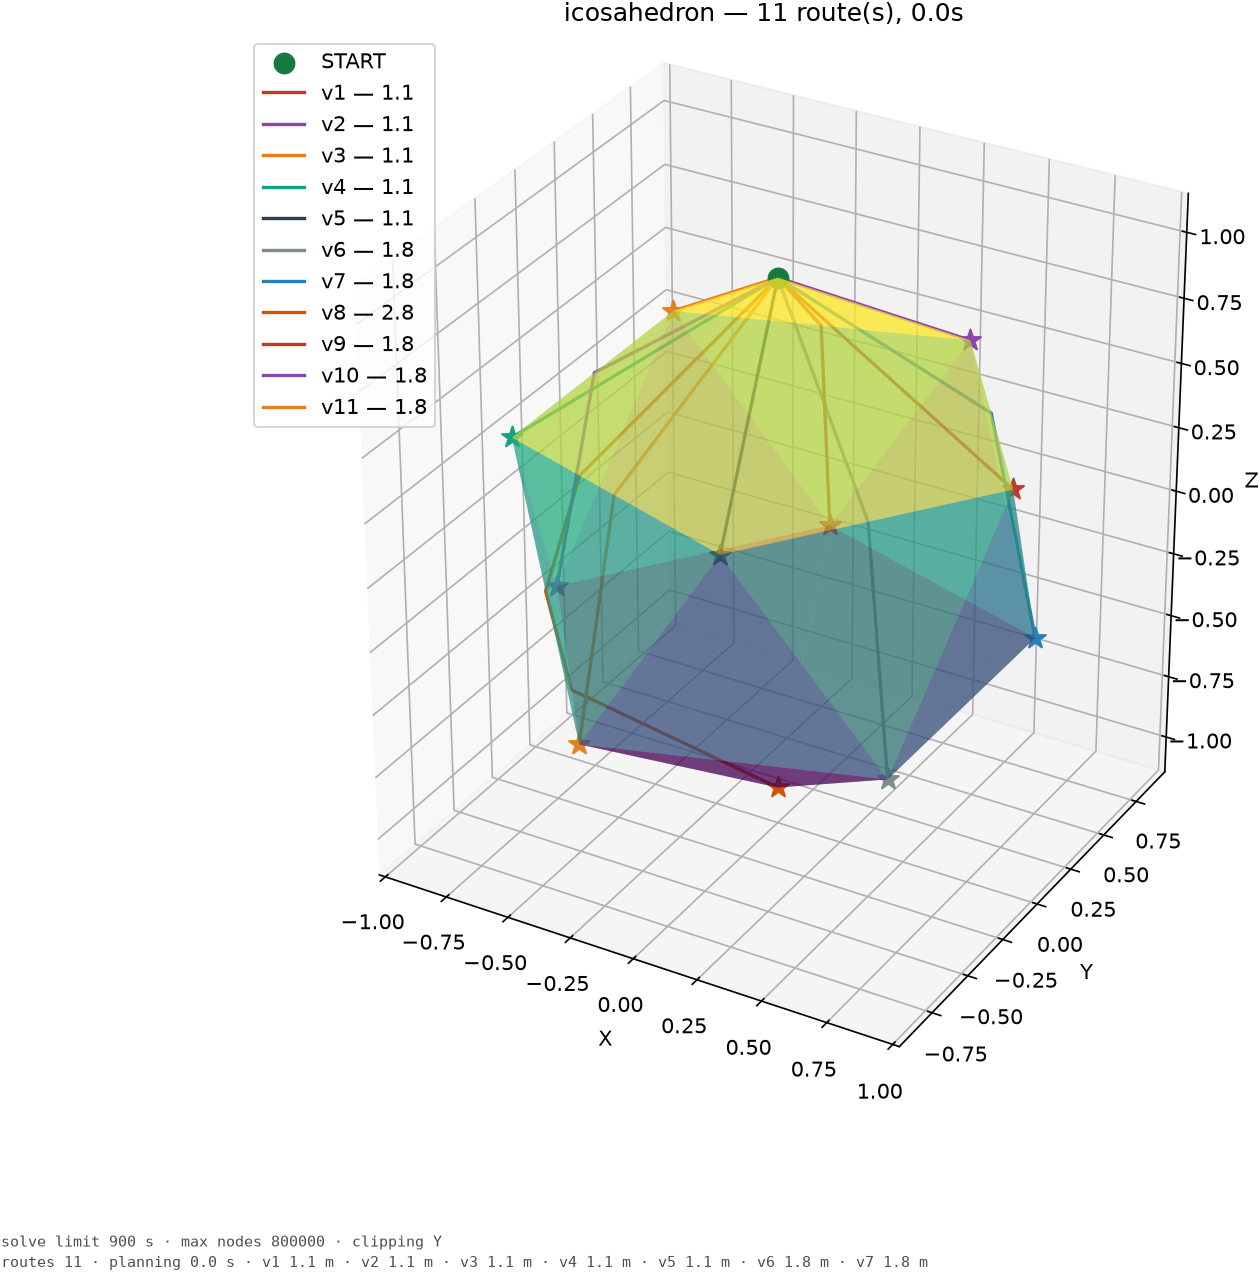
\includegraphics[width=0.9\linewidth]{Figures/crop/repo_icosahedron_routes.png}
  \caption{Các đường ngắn nhất từ đỉnh nguồn $s=0$ đến mọi đỉnh trên mặt
    icosahedron, do công cụ vẽ tuyến sinh từ route JSON của Funnel Tree. Funnel
    tree là cấu trúc sinh ra đồng thời tập đường này.}
  \label{fig:tree-icosa}
\end{figure}

Hình~\ref{fig:tree-icosa} cho thấy các tuyến tỏa từ đỉnh nguồn $s=0$ và đi qua
các mặt bên của icosahedron, không chỉ dọc theo cạnh. Một số tuyến gãy khúc tại
đỉnh có góc khuyết âm, đúng hành vi của đường trắc địa trên bề mặt lồi; đây cũng
là lý do funnel tree phải lan truyền qua mặt chứ không thể dùng đồ thị cạnh.

Đây là lựa chọn hợp lý cho bài toán giao hàng, vì funnel tree là cây ``một nguồn
đến mọi đích'', trùng trực tiếp với yêu cầu một kho hàng phục vụ nhiều khách hàng.

Về góc độ khoa học dữ liệu, bài toán là bài toán hình học -- tối ưu chứ không
phải bài toán dự đoán; phần đóng vai trò ``dữ liệu'' nằm ở khâu thực nghiệm và
đánh giá: lưới tam giác hóa (mesh) là dữ liệu vào, thời gian chạy và độ dài đường
đi là biến đo được, và việc kiểm chứng thuật toán là đối chiếu đầu ra với một
chuẩn độc lập.

\subsection{Phát biểu bài toán}

\subsubsection{Đầu vào và đầu ra}

Đầu vào của bài toán gồm:
\begin{itemize}
  \item \textbf{Bề mặt tam giác hóa} $P\subset\R^3$ gồm $n$ tam giác, cho dưới
    dạng tập đỉnh và tập mặt, mỗi cạnh kề đúng hai mặt (bề mặt kín) hoặc một mặt
    (biên của bề mặt mở);
  \item \textbf{Đỉnh nguồn} $s$;
  \item \textbf{Tập đỉnh đích} $V$ (toàn bộ đỉnh, hoặc tập con quy định trước).
\end{itemize}
Đầu ra tương ứng gồm:
\begin{itemize}
  \item Với mỗi $v\in V$: đường đi ngắn nhất toàn cục $SP(s,v)$ nằm trên $P$,
    hoặc chỉ độ dài $|SP(s,v)|$;
  \item Với bài toán đàn robot: với mỗi cặp (kho $s_i$, khách $m_j$), độ dài
    $|SP(s_i,m_j)|$ và tương ứng một lộ trình khả thi.
\end{itemize}
Độ phức tạp mục tiêu là $O(n^2)$ với $n$ là số tam giác \cite{an2024funnel}.

Bài toán này \textbf{không thuộc} nhóm phân loại, hồi quy, phân cụm, dự báo chuỗi
thời gian, gợi ý, phát hiện bất thường, xử lý ngôn ngữ tự nhiên hay thị giác máy
tính. Đây là bài toán \textbf{tìm đường đi ngắn nhất chính xác} (\emph{exact
shortest path}) trong hình học tính toán: kết quả là một đáp án đúng hay sai, có
thể đối chiếu với giá trị chính xác, không có khái niệm ``huấn luyện -- dự đoán''
hay ``độ chính xác của mô hình''.

Bản đồ thành phố được dựng thành bề mặt tam giác hóa, và trên đó các thành phần
của bài toán tổng quát được ánh xạ sang đề tài như Bảng~\ref{tab:anh-xa-de-tai}.

\begin{table}[!t]
  \caption{Ánh xạ từ bài toán chung sang đề tài.}
  \label{tab:anh-xa-de-tai}
  {\fontsize{7}{9.3}\selectfont
  \begin{tabular}{@{}>{\raggedright\arraybackslash}p{70pt}>{\raggedright\arraybackslash}p{118pt}@{}}
    \toprule
    \textbf{Thành phần bài toán} & \textbf{Tương ứng trong đề tài} \\
    \midrule
    Đỉnh nguồn $s$ & Vị trí kho hàng \\
    Đỉnh đích $v$ & Vị trí khách hàng \\
    Bề mặt tam giác hóa $P$ & Bản đồ, địa hình thành phố dưới dạng đa diện \\
    $SP(s,v)$ & Tuyến đường tối ưu từ kho đến khách \\
    $N$ nguồn đến $M$ đích & Đàn robot xuất phát từ nhiều kho phục vụ nhiều khách \\
    \bottomrule
  \end{tabular}}
\end{table}

\subsection{Mục tiêu nghiên cứu}

Mục tiêu tổng quát: lập trình một chương trình tính đường đi tối ưu cho đàn robot
xuất phát từ kho hàng đến các khách hàng trên bản đồ thành phố được dựng thành
bề mặt tam giác hóa. Các mục tiêu cụ thể, mỗi mục kèm tiêu chí kiểm chứng được,
được liệt kê trong Bảng~\ref{tab:muc-tieu}; cột trạng thái phản ánh kết quả trình
bày trong bài báo này.

\begin{table*}[!t]
  \caption{Mục tiêu nghiên cứu và tiêu chí kiểm chứng.}
  \label{tab:muc-tieu}
  {\fontsize{7}{8.6}\selectfont
  \setlength{\tabcolsep}{4pt}%
  \begin{tabular}{@{}c>{\raggedright\arraybackslash}p{150pt}>{\raggedright\arraybackslash}p{150pt}c@{}}
    \toprule
    \# & Mục tiêu cụ thể & Tiêu chí kiểm chứng & Trạng thái \\
    \midrule
    1 & Cài đặt thuật toán và Thủ tục 2 của funnel tree từ bài báo bằng Python &
      Chạy được trên toàn bộ bộ mesh kiểm thử; chỉ dùng NumPy cho mảng, không dùng
      thư viện hình học ngoài & $\checkmark$ \\
    \addlinespace
    2 & Kiểm chứng tính đúng bằng đối chiếu độc lập & (a) 5 mesh có reference
      độc lập, dung sai tương đối $10^{-4}$; (b) 4 mesh
      không có reference chỉ kiểm tra khả năng chạy và nhất quán nội tại &
      (a) $\checkmark$ \textbullet\ (b) $\triangle$ \\
    \addlinespace
    3 & Mở rộng thuật toán cho bề mặt mở & Xử lý biên nằm trong
      mã thuật toán; chạy được trên \texttt{dome} và \texttt{terrain},
      nhưng hai mesh này không có reference độc lập & $\triangle$ \\
    \addlinespace
    4 & Ghép thành bài toán nhiều nguồn -- nhiều đích cho đàn robot & Kết quả từng
      cặp (kho, khách) bằng giá trị tối ưu của cặp đó & $\times$ \\
    \addlinespace
    5 & Trực quan hóa đường đi và bản đồ thành phố & Có hình tái lập được từ mã
      nguồn đính kèm & $\checkmark$ \\
    \bottomrule
  \end{tabular}
  \vspace{2pt}

  \footnotesize\raggedright
  \emph{Chú thích cột trạng thái:} $\checkmark$~hoàn thành \textbullet{}
  $\triangle$~chưa kiểm chứng đầy đủ \textbullet{} $\times$~chưa thực hiện. Với
  mục tiêu~2, cách (a) chạy trong mã kiểm chứng; cách (b) và (c) mới ở dạng
  nguyên mẫu. Mục tiêu~3 đã kiểm chứng bằng cận trên trên hai lưới mở
  (\texttt{dome}, \texttt{terrain}) ở Mục~\ref{sec:results}.}
\end{table*}

\subsection{Cấu trúc bài báo}

Bài báo gồm các phần sau. Mục~\ref{sec:intro} giới thiệu bối cảnh, phát biểu bài
toán và mục tiêu nghiên cứu. Mục~\ref{sec:theory} trình bày kiến thức nền (bề mặt
đa diện, straightest geodesic, cấu trúc phễu), cơ sở khoa học dữ liệu, nguyên lý
thuật toán Funnel Tree cùng cơ chế cắt tỉa và các chỉ số đánh giá.
Mục~\ref{sec:data} mô tả các nguồn dữ liệu thực nghiệm, đặc tả Data Dictionary,
kết quả kiểm tra chất lượng dữ liệu, phân tích khám phá và các insight hình học.
Mục~\ref{sec:results} trình bày kết quả thực nghiệm trên các lưới đa diện, nghiên
cứu trường hợp điển hình trên địa hình vách dốc, kiểm định cơ chế cắt tỉa, phân
tích sai số số học và thảo luận. Mục~\ref{sec:gazebo} trình bày phần mô phỏng
Gazebo: dựng ba bề mặt dẫn đường từ mô hình thành phố, lập tuyến bằng Funnel Tree,
mô phỏng bám tuyến trong Gazebo và so sánh ba cấu hình lưới.
Mục~\ref{sec:concl} kết luận.

%% ---------------------------------------------------------------------
%% 02 - CƠ SỞ LÝ THUYẾT
%% ---------------------------------------------------------------------

\section{Cơ sở lý thuyết}\label{sec:theory}

\subsection{Kiến thức miền}

Bề mặt đa diện tam giác hóa là bề mặt $P$ của một polytope trong $\R^3$ (khối đa
diện --- bản ba chiều của đa giác: lập phương, lăng trụ, \ldots), được chia thành
$n$ tam giác. Hai điểm $a,b$ trên $P$ nối với nhau bằng một đường nằm trọn trên
$P$; trong số mọi đường đó có đường ngắn nhất, ký hiệu $SP(a,b)$. Khi xét trong
một tập con $S$ của bề mặt, ký hiệu $SP_S(a,b)$ nghĩa là đường ngắn nhất
\emph{bị giới hạn trong} $S$ \cite{an2024funnel}. Nghiên cứu giới hạn ở trường
hợp polytope lồi (nối hai điểm bất kỳ bằng đoạn thẳng luôn nằm trong khối);
trường hợp không lồi đi theo cách xử lý tương ứng mà bài báo ghi chú là mở rộng.

Với một đường $\gamma$ trên bề mặt, tại mỗi điểm $w$ của $\gamma$ đo góc trái
$\alpha_{wl}$ và góc phải $\alpha_{wr}$; $\gamma$ được gọi là \emph{straightest
geodesic} (trắc địa thẳng nhất) khi hai góc này bằng nhau tại mọi $w$, tức khi
trải phẳng ra thì $\gamma$ thành một đoạn thẳng, không gấp khúc. Hai tính chất
được dùng về sau:
\begin{enumerate}
  \item Mọi đường ngắn nhất từ nguồn $s$ đến một đỉnh đều là \emph{straightest
    geodesic}.
  \item Vì đường trái của một phễu chính là $SP(s,p)$ nên nó tự động là
    \emph{straightest geodesic} --- đây là chi tiết quyết định cho toàn bộ thuật
    toán.
\end{enumerate}

Cho một dãy $m\ge 2$ tam giác liền kề $f_1,\ldots,f_m$ (gộp thành vùng $S$), một
đỉnh $s$ của $f_1$, hai đỉnh $p,q$ ở hai đầu dãy sao cho khi nhìn theo hướng
$f_1\to f_m$ thì $SP(s,p)$ nằm bên trái $SP(s,q)$. Funnel $F_{p,q,S}$ là vùng $S$
bị giới hạn bởi ba đường $SP(s,p)\cup SP(s,q)\cup SP(p,q)$ \cite{an2024funnel}.
Các thành phần của phễu được liệt kê trong Bảng~\ref{tab:thanh-phan-funnel}.

\begin{table}[!t]
  \caption{Các thành phần của một phễu.}
  \label{tab:thanh-phan-funnel}
  {\fontsize{7}{9.3}\selectfont
  \begin{tabular}{@{}>{\raggedright\arraybackslash}p{58pt}>{\raggedright\arraybackslash}p{126pt}@{}}
    \toprule
    \textbf{Thuật ngữ} & \textbf{Ý nghĩa} \\
    \midrule
    Cusp (đỉnh chụm) $s$ & Gốc của phễu; với polytope lồi, hai biên chỉ giao nhau
      tại $s$ \\
    Left border $SP(s,p)$ & Biên trái; luôn là \emph{straightest geodesic} \\
    Right border $SP(s,q)$ & Biên phải \\
    Direct destination $v$ & Đỉnh nằm ngoài $S$ nhưng kề cạnh với $q$ --- đích mà
      phễu có thể ``vươn tới'' \\
    \bottomrule
  \end{tabular}}
\end{table}

Hình~\ref{fig:funnel-cusp} minh họa cấu trúc này bằng một sơ đồ phẳng: vùng tam
giác $S$ giữa hai biên, cusp $s$, hai biên $SP(s,p)$ và $SP(s,q)$, cùng cạnh
$[q,v]$ dẫn tới đỉnh đích $v$.

\begin{figure}[!t]
  \centering
  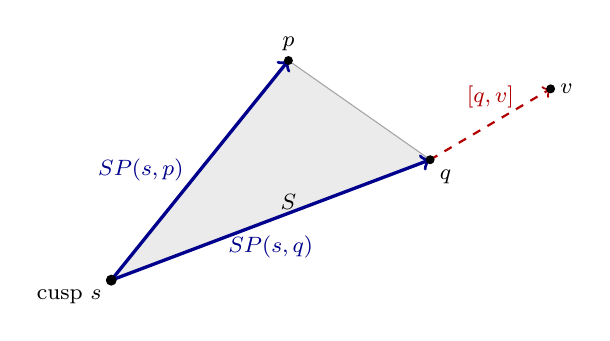
\begin{tikzpicture}[scale=0.9, every node/.style={font=\footnotesize}]
    \coordinate (s) at (0,0);
    \coordinate (p) at (2.5,3.1);
    \coordinate (q) at (4.5,1.7);
    \coordinate (v) at (6.2,2.7);
    \fill[black!8] (s) -- (p) -- (q) -- cycle;
    \draw[black!35] (p) -- (q);
    \draw[very thick, blue!55!black, ->] (s) -- (p)
      node[midway, left=2pt] {$SP(s,p)$};
    \draw[very thick, blue!55!black, ->] (s) -- (q)
      node[midway, below=2pt] {$SP(s,q)$};
    \draw[thick, red!70!black, dashed, ->] (q) -- (v)
      node[midway, above=2pt] {$[q,v]$};
    \fill (s) circle (2.2pt) node[below left] {cusp $s$};
    \fill (p) circle (1.8pt) node[above] {$p$};
    \fill (q) circle (1.8pt) node[below right] {$q$};
    \fill (v) circle (1.8pt) node[right] {$v$};
    \node at (2.5,1.1) {$S$};
  \end{tikzpicture}
  \caption{Cấu trúc phễu: cusp $s$, left border $SP(s,p)$, right border $SP(s,q)$
    và cạnh $[q,v]$ dẫn tới direct destination $v$. Đây là sơ đồ khái niệm, không
    phải ảnh kết quả từ repo.}
  \label{fig:funnel-cusp}
\end{figure}

Hình~\ref{fig:funnel-cusp} cho thấy vùng $S$ nằm giữa hai biên, cusp $s$ là nơi
hai biên gặp nhau, và cạnh $[q,v]$ là lối duy nhất để phễu vươn sang tam giác kề.
Khi phễu mở rộng, biên trái $SP(s,p)$ vẫn là đường trắc địa thẳng nhất; đây là
bất biến mà các bước so sánh góc và độ dài dựa vào.

Từ một phễu, khi mở rộng vùng $S$ bằng các tam giác kề cạnh $[q,v]$ ta được các
phễu con (\emph{child}); quan hệ con -- cha này dựng nên một cây có gốc là $s$,
gọi là \textbf{funnel tree}. Mỗi nút của cây là một cặp (phễu, $SP_S(p,q)$); khi
cây hoàn chỉnh, mỗi đường ngắn nhất $SP(s,v)$ ứng với đúng một nút trong cây, nên
việc dựng cây đồng thời tính ra mọi đường ngắn nhất từ $s$ \cite{an2024funnel}.

Một cách tiếp cận truyền thống là trải phẳng (\emph{planar unfolding}): ``mở'' các
tam giác xuống mặt phẳng sao cho giữ nguyên chiều dài cạnh; trên mặt phẳng, đường
ngắn nhất là đoạn thẳng nên dễ tính bằng tọa độ. Nhược điểm là mỗi lần mở lại phải
chuỗi theo một loạt phép biến hình đẳng cự, và khi cửa sổ (\emph{window}) di
chuyển qua các tam giác thì phải cập nhật lại. Toàn bộ nhánh Chen -- Han dùng kỹ
thuật này.

\subsection{Cơ sở khoa học dữ liệu}

Nghiên cứu không có mô hình học máy để huấn luyện: không có tập huấn luyện, tập
kiểm thử và không dự đoán nhãn. Vì vậy phần ``khoa học dữ liệu'' nằm ở quy trình
đo lường và kiểm chứng, tương tự một thực nghiệm tính toán (\emph{computational
experiment}):
\begin{description}
  \item[Dữ liệu vào] bộ mesh --- mỗi mesh là một tập cấu trúc (tập đỉnh, tập mặt,
    quan hệ kề), sinh bằng mã nguồn trong nghiên cứu; đặc trưng của từng mesh (số
    đỉnh, số mặt, độ cao, số cạnh biên) được mô tả ở Mục~\ref{sec:data}.
  \item[Biến đo được] độ dài đường đi $|SP(s,v)|$, sai số tương đối so với
    reference, số lần lan truyền $P$, thời gian chạy và các sai số bám tuyến từ
    telemetry.
  \item[Chuẩn đối chiếu] vì đây là bài toán có đáp án chính xác, ``nhãn'' thay thế
    bằng các polyline tham chiếu độc lập cho 5 mesh nhỏ. Bốn mesh không có reference và bề mặt thành phố không có bộ giải độc lập
    trong repo, nên chỉ được kiểm tra khả năng chạy và tính nhất quán nội tại.
    Quy trình: sinh mesh $\to$ chạy thuật toán $\to$ đối chiếu độ dài với reference
    $\to$ tổng hợp thành bảng số liệu.
\end{description}

Cách đặt này cũng giải thích vì sao các chỉ số quen thuộc của bài toán phân loại
(Accuracy, F1, ROC-AUC) \textbf{không áp dụng} ở đây: không tồn tại dự đoán sai
lệch xác suất để đo, chỉ có sai số giữa hai giá trị số thực.

\subsection{Các thuật toán sử dụng}

Theo Phan, Hoai và Thinh, nhánh phương pháp Chen và Han duy trì các cửa sổ trên bề
mặt đã trải phẳng và lan truyền chúng qua các mặt kề nhau; đây là cơ sở để bài
báo đối sánh với Funnel Tree \cite{an2024funnel}.

Thuật toán chính của bài báo \cite{an2024funnel} thay bước trải phẳng bằng
\textbf{so sánh góc trực tiếp trên khối ba chiều}, nhờ hai dữ kiện ở mục trên:
left border là \emph{straightest geodesic}, nên hình học của phễu xác định được
bằng định luật cos
\begin{equation}
  c=\sqrt{a^2+b^2-2ab\cos\theta}.
  \label{eq:cosine}
\end{equation}
Thuật toán gồm hai phần:
\begin{itemize}
  \item \textbf{Algorithm 1 (dựng cây):} từ cusp $s$, cây lớn dần theo từng tầng.
    Với mỗi phễu $F_{p,q,S}$ và mỗi direct destination $v$, tính góc $\beta_v$
    bằng \eqref{eq:cosine} rồi rẽ nhánh theo hai điều kiện: (5) $\beta_v<\pi$ ---
    nếu không thỏa thì phần trong của phễu con rỗng và dừng lại; (6)
    $\angle psv<\angle psw$ --- nếu thỏa thì sinh hai con, không thì một con. Mỗi
    phễu chỉ tốn $O(1)$ phép so sánh, tổng số nút của cây là $O(n^2)$ nên độ phức
    tạp thời gian và bộ nhớ đều là $O(n^2)$.
  \item \textbf{Thủ tục 2 (clip off funnels):} xử lý trường hợp hai phễu cùng cusp
    cùng ``chiếm'' một đỉnh (\emph{occupy a vertex}) --- khi đó đỉnh đó bị loại ra
    khỏi cây cho đến khi phễu được mở rộng đầy đủ rồi mới gán lại, để duy trì tính
    đúng đắn và giới hạn số nút. Trong thực tế các đỉnh bị loại rất ít.
\end{itemize}
Trong cài đặt, mỗi nút của cây lưu một bộ ba số $(x,y,z)$ lần lượt là góc tại
cusp, độ dài left border $|sp|$ và góc $\angle spq$ \cite{an2024funnel} --- chính
ba đại lượng mà \eqref{eq:cosine} cần.

Ba đoạn mã dưới đây là lõi của Thuật toán 1 và Thủ tục 2 trong cài đặt Python của
nghiên cứu \cite{quangnguyen2025} ($\beta_v$, $\angle psv$, $\angle pvw$ là các
đại lượng ký hiệu như trong bài báo): Mã~\ref{code:alg1} dựng cây theo từng tầng
(đúng dòng 5--18 của Thuật toán 1), Mã~\ref{code:alg1-expand} là phần mở rộng
từng phễu --- nơi chứa các điều kiện rẽ nhánh (5) và (6), và Mã~\ref{code:clip2}
triển khai Thủ tục 2.

\begin{code}[!t]
  \lstinputlisting[style=pycode]{Code/funnel_tree.py}
  \caption{Thuật toán 1 (\texttt{funnel\_tree.py}): dựng funnel tree gốc $s$.}
  \label{code:alg1}
\end{code}

\begin{code}[!t]
  \lstinputlisting[style=pycode]{Code/funnel_expand.py}
  \caption{Thuật toán 1 (\texttt{funnel\_expand.py}): mở rộng một phễu.}
  \label{code:alg1-expand}
\end{code}

\begin{code}[!t]
  \lstinputlisting[style=pycode]{Code/funnel_clip.py}
  \caption{Thủ tục 2 (\texttt{funnel\_clip.py}): clip off funnels.}
  \label{code:clip2}
\end{code}

Sau khi lan truyền, polyline ứng viên được tái dựng bằng cách trải phẳng dải mặt
đã chọn; đây là một khác biệt cần nêu rõ so với mục tiêu xử lý hoàn toàn nội tại
trong phương pháp gốc. Đối với bề mặt có cấu hình không lồi, bản triển khai xét
thêm các nguồn phụ tại những đỉnh có tổng góc mặt vượt $2\pi$ theo ngưỡng số của
chương trình, rồi ghép các đoạn đường giữa nguồn và đích thông qua một đồ thị có
trọng số. Đồ thị này được tìm kiếm bằng A* với heuristic
$h(v)=\norm{v-g}$; khoảng cách thẳng trong $\R^3$ là cận dưới cho độ dài một đường
bị ràng buộc nằm trên bề mặt, nên A* chỉ dùng để chọn các đoạn ứng viên trong đồ
thị nguồn phụ, không thay bề mặt bằng đồ thị cạnh tam giác đơn thuần. Sau tái dựng,
chương trình kiểm tra đường thuộc lưới và kiểm tra tính nhất quán giữa độ dài lan
truyền với độ dài polyline. Việc tìm được đường trên đồ thị nguồn phụ chưa tự
chứng minh đường đó tối ưu trên toàn bề mặt; bước đối chiếu với chương trình tham
chiếu được thực hiện riêng.

Bảng~\ref{tab:chenhan-vs-funnel} tóm tắt đối sánh hai nhánh theo bài báo gốc
\cite{an2024funnel}.

\begin{table}[!t]
  \caption{So sánh nhóm Chen -- Han và funnel tree.}
  \label{tab:chenhan-vs-funnel}
  {\fontsize{7}{8.6}\selectfont
  \begin{tabular}{@{}>{\raggedright\arraybackslash}p{48pt}>{\raggedright\arraybackslash}p{66pt}>{\raggedright\arraybackslash}p{66pt}@{}}
    \toprule
    \textbf{Tiêu chí} & \textbf{Chen và Han (1996)} & \textbf{Funnel tree (2024)} \\
    \midrule
    Độ phức tạp & $O(n^2)$ & $O(n^2)$ \\
    Trải phẳng & Có --- mỗi cửa sổ một chuỗi phép biến hình & Không --- so sánh
      góc bằng định luật cos trên ba chiều \\
    Nguồn ảnh, phép chiếu & Có & Không \\
    Kỹ thuật & Lan truyền cửa sổ trên mặt phẳng & Phễu và \emph{straightest
      geodesic} \\
    Số nút trên \texttt{cube4} & \num{1287379} & \num{10401} \\
    Hiệu năng thực nghiệm & Tham chiếu & Nhanh hơn 1 đến 12 lần \\
    \bottomrule
  \end{tabular}}
\end{table}

Funnel tree được chọn vì ba lý do: (i) cây một nguồn -- mọi đích trùng khớp trực
tiếp với yêu cầu kho -- mọi khách; (ii) cùng độ phức tạp $O(n^2)$ nhưng ít phép
toán hơn; (iii) cài đặt bằng Python gọn, chỉ cần NumPy cho mảng và thư viện chuẩn,
không cần thư viện hình học. Kết quả cài đặt được đối chiếu với các đầu ra tham
chiếu đi kèm bộ mã nguồn của nghiên cứu \cite{quangnguyen2025}.

\subsection{Chỉ số đánh giá}

Vì là bài toán tìm đường đúng -- sai, các chỉ số là các đại lượng số thực giữa đáp
án của thuật toán và giá trị tham chiếu, được liệt kê trong
Bảng~\ref{tab:chi-so-danh-gia}.

\begin{table*}[!t]
  \caption{Các chỉ số đánh giá.}
  \label{tab:chi-so-danh-gia}
  {\fontsize{7}{8.6}\selectfont
  \setlength{\tabcolsep}{4pt}%
  \begin{tabular}{@{}>{\raggedright\arraybackslash}p{70pt}>{\raggedright\arraybackslash}p{160pt}>{\raggedright\arraybackslash}p{150pt}@{}}
    \toprule
    \textbf{Chỉ số} & \textbf{Định nghĩa} & \textbf{Vai trò} \\
    \midrule
    Độ dài đường đi & $\norm{SP(s,v)}$ --- độ dài đường ngắn nhất trên bề mặt &
      kết quả chính của thuật toán \\
    \addlinespace
    Sai số tương đối & $\varepsilon=\bigl|\,\norm{SP}-d_{\text{ref}}\,\bigr|/d_{\text{ref}}$
      so với đường tham chiếu & đối chiếu 5 mesh có reference \\
    \addlinespace
    Số lần lan truyền & $P$ --- số lần gọi \texttt{propagate} trong một lượt tìm &
      đo quy mô tìm kiếm \\
    \addlinespace
    Thời gian lập tuyến & giây, gồm đọc mesh và ghi JSON & số liệu quan sát, không
      dùng làm benchmark \\
    \addlinespace
    Sai số bám tuyến & $e_{\max}$, $\bar e$, $e_{\rm final}$ từ telemetry &
      đánh giá chuyến bay \\
    \addlinespace
    Hợp lệ / đạt mốc & hết tuyến và $e_{\rm final}\le0{,}5$ / thêm
      $e_{\max}\le1{,}0$ & hai tiêu chí tách riêng \\
    \bottomrule
  \end{tabular}}
\end{table*}

Sai số tương đối với chuẩn, khi cần, được tính theo
$\varepsilon=\bigl|\,\norm{SP}-d_{\text{chuẩn}}\,\bigr|/d_{\text{chuẩn}}$. Các
chỉ số Accuracy, Precision, Recall, F1, ROC-AUC \emph{không} được dùng vì không
có tập dự đoán phân loại.

%% ---------------------------------------------------------------------
%% 03 - DỮ LIỆU THỰC NGHIỆM VÀ PHÂN TÍCH KHÁM PHÁ
%% ---------------------------------------------------------------------

\section{Dữ liệu thực nghiệm và phân tích khám phá}\label{sec:data}

Bài toán của nghiên cứu là bài toán hình học -- tối ưu trong không gian ba chiều,
không thuộc lớp bài toán học máy có giám sát: ``dữ liệu'' ở đây là các \textbf{bề
mặt đa diện tam giác hóa} (mesh) mà đường đi ngắn nhất trắc địa được tính toán
trên đó, kèm theo các tập \textbf{kết quả tham chiếu} dùng để đối chiếu và kiểm
chứng tính đúng đắn của thuật toán.

Toàn bộ dữ liệu thực nghiệm, mã nguồn thuật toán và công cụ hỗ trợ được công khai
tại \cite{kien2026repo}. Dữ liệu được tổ chức thành ba lớp: \emph{nguồn gốc} gồm
9 mesh \texttt{.off} và scene thành phố \texttt{city.glb}; \emph{đã xử lý} gồm
mesh đã kiểm tra, bề mặt dẫn đường và mission START/GOAL; và \emph{tham chiếu} gồm
5 tệp polyline cho các mesh nhỏ. Kết quả của mỗi lần chạy được lưu riêng, không
ghi đè lên lần trước. Đường dẫn tệp cụ thể nằm ở Phụ lục A.

Mục này mô tả chi tiết hai nguồn dữ liệu thực nghiệm, định dạng và data dictionary
của chúng, kết quả kiểm tra chất lượng dữ liệu, phân tích khám phá (EDA) kèm trực
quan hóa hình ảnh không gian 3D, từ đó rút ra các insight ảnh hưởng trực tiếp tới
khâu đánh giá thực nghiệm ở Mục~\ref{sec:results}.

\subsection{Nguồn dữ liệu}

\begin{enumerate}
\item Bộ mesh kiểm thử gồm 9 tệp \texttt{.off} dạng văn bản thuần:
\begin{itemize}
  \item 5 mesh mẫu có đường tham chiếu độc lập dùng để đối chiếu kết quả: \texttt{J17}, \texttt{L}, \texttt{cliff},
    \texttt{demo\_mesh}, \texttt{star}. Đây là các mesh tổng hợp nhỏ (khối đa diện
    lồi, ``đồi vách dốc'', lưới mẫu không lồi).
  \item 2 mesh dựng lại theo hình minh họa của bài báo gốc \cite{an2024funnel}:
    \texttt{cube} (Hình~7 của bài báo) và \texttt{icosahedron} (Hình~4 của bài
    báo).
  \item 2 mesh mở rộng cho bề mặt mở: \texttt{dome} (mảnh vỏ cầu hở khuyết đáy có
    8 cạnh biên) và \texttt{terrain} (mô hình địa hình có thung lũng lõm và 24
    cạnh biên).
  \item kèm theo là file mô hình thành phố \texttt{city.glb} (khoảng 20,5 MB, mô
    hình 3D định dạng glTF/GLB), được dùng cho quy trình mô phỏng ở
    Mục~\ref{sec:gazebo}.
\end{itemize}

\item Kết quả tham chiếu gồm 5 tệp JSON cho các mesh \texttt{cliff},
  \texttt{demo\_mesh}, \texttt{J17}, \texttt{L} và \texttt{star}; mỗi tệp ghi
  \texttt{mesh}, \texttt{source},
  \texttt{coordinate\_system} và danh sách \texttt{paths}; \texttt{paths[i]} là
  polyline ngắn nhất từ đỉnh nguồn tới đỉnh $i$, tọa độ các điểm uốn trắc địa làm
  tròn 4 chữ số thập phân. Hai mesh \texttt{cube} và \texttt{icosahedron} được
  dựng theo hình vẽ của bài báo gốc, còn \texttt{dome} và \texttt{terrain} là hai
  bề mặt mở; bốn mesh này không có file tham chiếu độc lập trong repo, nên được
  dùng để kiểm tra khả năng chạy và tính nhất quán nội tại chứ không đối chiếu
  từng đỉnh.
\end{enumerate}

Bộ mesh kiểm thử có tính đại diện vì gồm các mesh tổng hợp với kích thước từ 7 đến
49 đỉnh. Mặc dù nhỏ hơn quy mô 100--800 đỉnh trong bài báo \cite{an2024funnel},
tập dữ liệu này bao quát đầy đủ các dạng cấu trúc hình học đặc trưng: đa diện lồi,
bề mặt không lồi, bề mặt có lỗ (xuyến $\chi=0$) và bề mặt mở có cạnh biên
($\chi=1$). Nhờ đó, tập dữ liệu đáp ứng yêu cầu kiểm chứng tính đúng đắn và độ ổn
định của thuật toán.

\subsection{Mô tả dữ liệu và Data Dictionary}

File đầu vào có định dạng \texttt{.off} và được đọc bởi một hàm đọc mesh duy nhất.
Dòng đầu là \texttt{OFF}; dòng thứ hai gồm ba số
nguyên \texttt{V F E} ($V$ = số đỉnh, $F$ = số mặt tam giác, $E$ = số cạnh); tiếp
theo là $V$ dòng tọa độ thực \texttt{x y z}; cuối cùng là $F$ dòng tam giác
\texttt{3 i j k} (ba chỉ số đỉnh, đánh chỉ mục từ 0). Trường $E$ trong một số file
không chính xác và được tính lại từ danh sách tam giác. Kết quả tham chiếu có định
dạng JSON, trong đó mỗi phần tử của danh sách \texttt{paths} là một polyline 3D ứng với một đỉnh đích; tọa độ được làm tròn 4
chữ số thập phân.

Vì dữ liệu là mesh đa diện 3D chứ không phải bảng dữ liệu quan sát dạng dòng/cột
truyền thống, các ``biến'' ở đây là các \textbf{đặc trưng cấu trúc hình học và tô
pô của mesh}. Bảng~\ref{tab:data-dictionary} định nghĩa chi tiết Data Dictionary.

\begin{table*}[!t]
  \caption{Data Dictionary của bộ mesh kiểm thử.}
  \label{tab:data-dictionary}
  {\fontsize{7}{8.6}\selectfont
  \setlength{\tabcolsep}{3pt}%
  \begin{adjustbox}{max width=\textwidth}
  \begin{tabular}{@{}>{\raggedright\arraybackslash}p{54pt}
                  >{\raggedright\arraybackslash}p{52pt}
                  >{\raggedright\arraybackslash}p{146pt}
                  >{\raggedright\arraybackslash}p{36pt}
                  >{\raggedright\arraybackslash}p{104pt}@{}}
    \toprule
    \textbf{Biến} & \textbf{Kiểu dữ liệu} & \textbf{Ý nghĩa} & \textbf{Đơn vị} &
    \textbf{Vai trò} \\
    \midrule
    \texttt{name} & chuỗi & tên file mesh (\texttt{cliff.off}, \ldots) & --- &
      định danh \\
    $V$ & nguyên & số đỉnh của mesh & đỉnh & quy mô; chi phối độ phức tạp
      $O(V^2)$ \\
    $F$ & nguyên & số mặt tam giác & tam giác & quy mô \\
    $E$ & nguyên & số cạnh khác nhau (tính từ danh sách tam giác) & cạnh & kiểm tra
      nhất quán Euler \\
    $\chi=V-E+F$ & nguyên & số Euler & --- & phân loại bề mặt (kín, mở, xuyến) \\
    \texttt{boundary} & nguyên & số cạnh chỉ kề đúng 1 tam giác & cạnh & phát hiện
      bề mặt mở \\
    \texttt{components} & nguyên & số thành phần liên thông & --- & kiểm mesh rời
      rạc \\
    \texttt{span} & thực & độ rộng theo từng trục ($\max-\min$ tọa độ) & đơn vị
      mesh & phát hiện khác thang đo \\
    $s$ & nguyên & chỉ số đỉnh nguồn (0-based) & --- & điều kiện đầu vào của mỗi
      thí nghiệm \\
    \texttt{has\_expected} & logic & có đường tham chiếu độc lập hay không &
      --- & xác định phạm vi kiểm chứng \\
    \bottomrule
  \end{tabular}
  \end{adjustbox}}
\end{table*}

Bảng~\ref{tab:dac-trung-mesh} áp dụng Data Dictionary này cho toàn bộ 9 mesh kiểm
thử \cite{kien2026repo}.

\begin{table*}[!t]
  \caption{Đặc trưng hình học và tô pô của 9 mesh kiểm thử.}
  \label{tab:dac-trung-mesh}
  {\fontsize{7}{8.6}\selectfont
  \setlength{\tabcolsep}{2.5pt}%
  \begin{adjustbox}{max width=\textwidth}
  \begin{tabular}{@{}lrrrrrlr@{}}
    \toprule
    \textbf{Mesh} & $V$ & $F$ & $E$ & $\chi$ & \textbf{Cạnh biên} &
    \textbf{Dạng bề mặt} & \textbf{Tham chiếu} \\
    \midrule
    \texttt{cliff}        & 7  & 10 & 15  & 2 & 0  & Kín (cầu)       & \texttt{paths.json} \\
    \texttt{cube}         & 8  & 12 & 18  & 2 & 0  & Kín (lồi)       & Không có \\
    \texttt{J17}          & 10 & 16 & 24  & 2 & 0  & Kín (cầu)       & \texttt{paths.json} \\
    \texttt{L}            & 12 & 20 & 30  & 2 & 0  & Kín (cầu)       & \texttt{paths.json} \\
    \texttt{icosahedron}  & 12 & 20 & 30  & 2 & 0  & Kín (lồi đều)   & Không có \\
    \texttt{star}         & 16 & 28 & 42  & 2 & 0  & Kín (không lồi) & \texttt{paths.json} \\
    \texttt{dome}         & 25 & 40 & 64  & 1 & 8  & Mở (vỏ cầu)     & Không có \\
    \texttt{demo\_mesh}   & 31 & 62 & 93  & 0 & 0  & Kín (xuyến)     & \texttt{paths.json} \\
    \texttt{terrain}      & 49 & 72 & 120 & 1 & 24 & Mở (địa hình)   & Không có \\
    \bottomrule
  \end{tabular}
  \end{adjustbox}
  \vspace{2pt}

  \footnotesize\raggedright
  Cột $\chi=V-E+F$ là số Euler. ``Không có'' nghĩa là mesh không có file tham
  chiếu độc lập; các mesh này được dùng để kiểm tra
  khả năng chạy trên bề mặt lồi, bề mặt mở và bề mặt có lỗ, không đối chiếu từng
  đỉnh.}
\end{table*}

\subsection{Đánh giá chất lượng dữ liệu}

Các kiểm tra tự động trên cả 9 file đầu vào (thực hiện bởi bộ đọc mesh và bộ lập
tuyến):
\begin{description}
  \item[Cấu trúc hợp lệ] Mọi dòng tam giác đều có dạng \texttt{3 i j k} với
    $0\le i,j,k<V$; không có chỉ số đỉnh nào nằm ngoài phạm vi, không có tam giác
    nào bị thiếu đỉnh.
  \item[Trùng lặp và nhiễu] Không có đỉnh trùng tọa độ trên cả 9 mesh; không có tam
    giác thoái hóa --- diện tích tam giác nhỏ nhất trong toàn bộ dữ liệu là 0,0920
    (đơn vị vuông, trên \texttt{dome}), lớn hơn nhiều ngưỡng zero số học $10^{-12}$.
  \item[Tính hình học 2-manifold] Không có cạnh nào kề quá 2 tam giác (mesh phi đa
    tạp bằng 0); mỗi mesh tạo thành một thành phần liên thông hoàn chỉnh duy nhất.
  \item[Phân loại bề mặt kín và mở] Có 7 mesh là bề mặt kín hoàn toàn với 0 cạnh
    biên (trong đó 6 mesh có $\chi=2$ dạng cầu và \texttt{demo\_mesh} có $\chi=0$
    dạng xuyến có lỗ rỗng xuyên tâm). Hai mesh còn lại là bề mặt mở: \texttt{dome}
    có 8 cạnh biên và \texttt{terrain} có 24 cạnh biên, cả hai đều đạt số đặc
    trưng Euler $\chi=1$ đúng với cấu trúc bề mặt mở có một chu vi biên liên tục.
  \item[Nhất quán số Euler] Với mọi mesh, giá trị $V-E+F$ tính từ dữ liệu khớp
    chính xác tuyệt đối với $\chi$ ở Bảng~\ref{tab:dac-trung-mesh} (2, 1 hoặc 0),
    không xảy ra sai lệch tô pô ở bất kỳ mô hình nào.
  \item[Lỗi vô hại ở header file] Số thứ ba của dòng đầu (cột $E$ theo quy ước gốc)
    không phải lúc nào cũng chính xác trong file văn bản: ví dụ \texttt{L.off} ghi
    10 (thực tế $E=30$), \texttt{demo\_mesh.off} ghi 0 (thực tế 93). Mã nguồn đọc
    file tự động suy ra danh sách cạnh thực tế từ các mặt tam giác nên sai lệch ở
    header hoàn toàn vô hại đối với thuật toán.
  \item[Khác biệt thang đo tọa độ] 8 mesh có tọa độ trong khoảng đơn vị nhỏ, cỡ
    $[-3,5]$; riêng \texttt{demo\_mesh} trải trên $x\in[26,344]$, $y\in[-320,550]$,
    $z\in[-288,207]$ --- độ rộng lớn gấp khoảng 100 lần. Do đó, sai số tuyệt đối
    giữa các mesh không thể so sánh gộp chung mà phải dùng sai số tương đối.
\end{description}

Về tập kết quả tham chiếu, 5/9 mesh có file \texttt{.paths.json} trong
tham chiếu; bốn mesh còn lại (\texttt{cube}, \texttt{icosahedron},
\texttt{dome}, \texttt{terrain}) không có tham chiếu độc lập. Công cụ
bước đối chiếu chạy Funnel Tree từ đúng đỉnh nguồn ghi trong
reference, so độ dài từng polyline với dung sai tương đối $10^{-4}$ và hiện báo
0 failure trên tổng 76 đỉnh; sai số tương đối lớn nhất là $1{,}7\times10^{-5}$
(\texttt{cliff}), phát sinh từ việc reference chỉ giữ bốn chữ số thập phân. Với
bốn mesh không có reference, kết quả chỉ được kiểm tra nhất quán nội tại: độ dài
polyline dựng lại phải khớp độ dài nội tại mà phép lan truyền tính được, chứ
không có đối chiếu với một bộ giải thứ hai.

\subsection{Exploratory Data Analysis và trực quan hóa}

Trước khi thực hiện các phép đo chi tiết, quy trình EDA đặt ra bốn câu hỏi then
chốt đối với tập dữ liệu:
\begin{enumerate}
  \item Bộ mesh bao gồm những dạng hình học và đặc trưng tô pô nào (kín/mở,
    lồi/không lồi, có lỗ rỗng)?
  \item Quy mô đỉnh và mặt của từng mesh ra sao, có đủ đa dạng để đánh giá thuật
    toán không?
  \item Các mesh có cùng thang đo tọa độ không gian không?
  \item Nguồn kiểm chứng chuẩn phủ bao nhiêu phần của bộ mesh?
\end{enumerate}
Tổng hợp từ Bảng~\ref{tab:dac-trung-mesh} và phần phân tích chất lượng dữ liệu:
\begin{description}
  \item[Đặc trưng tô pô (Q1)] Đa dạng cao: 7 mesh kín (6 dạng cầu $\chi=2$, 1 dạng
    xuyến $\chi=0$) và 2 mesh mở có cạnh biên ($\chi=1$).
  \item[Quy mô mesh (Q2)] Số đỉnh $V$ trải từ 7 đến 49 (trung vị 12), số mặt $F$
    từ 10 đến 72 (trung vị 20), số cạnh $E$ từ 15 đến 120. Tập mesh có độ dãn quy
    mô hợp lý để kiểm chứng thuật toán từ đơn giản đến phức tạp.
  \item[Thang đo không gian (Q3)] 8 mesh dùng bậc đơn vị cỡ 1--5; riêng
    \texttt{demo\_mesh} dùng bậc $10^2$ (lệch khoảng 100 lần).
  \item[Phủ chuẩn kiểm chứng (Q4)] 5 mesh có file tham chiếu
    đường tham chiếu; 4 mesh còn lại (\texttt{cube},
    \texttt{icosahedron}, \texttt{dome}, \texttt{terrain}) chỉ kiểm tra được
    khả năng chạy và tính nhất quán nội tại.
\end{description}

Các hình dưới đây được kết xuất trực tiếp từ công cụ trực quan hóa của quy
trình; mỗi ảnh có chân ghi tham số, số đỉnh/mặt và SHA của mesh.
Hình~\ref{fig:closed-meshes} trực quan hóa ba mô hình lưới đa diện kín tiêu biểu:
khối đa diện lồi đều \texttt{icosahedron}, mô hình vách dốc \texttt{cliff} và khối
sao không lồi \texttt{star}.

\begin{figure*}[!t]
  \centering
  \begin{subfigure}{0.46\textwidth}
    \centering
    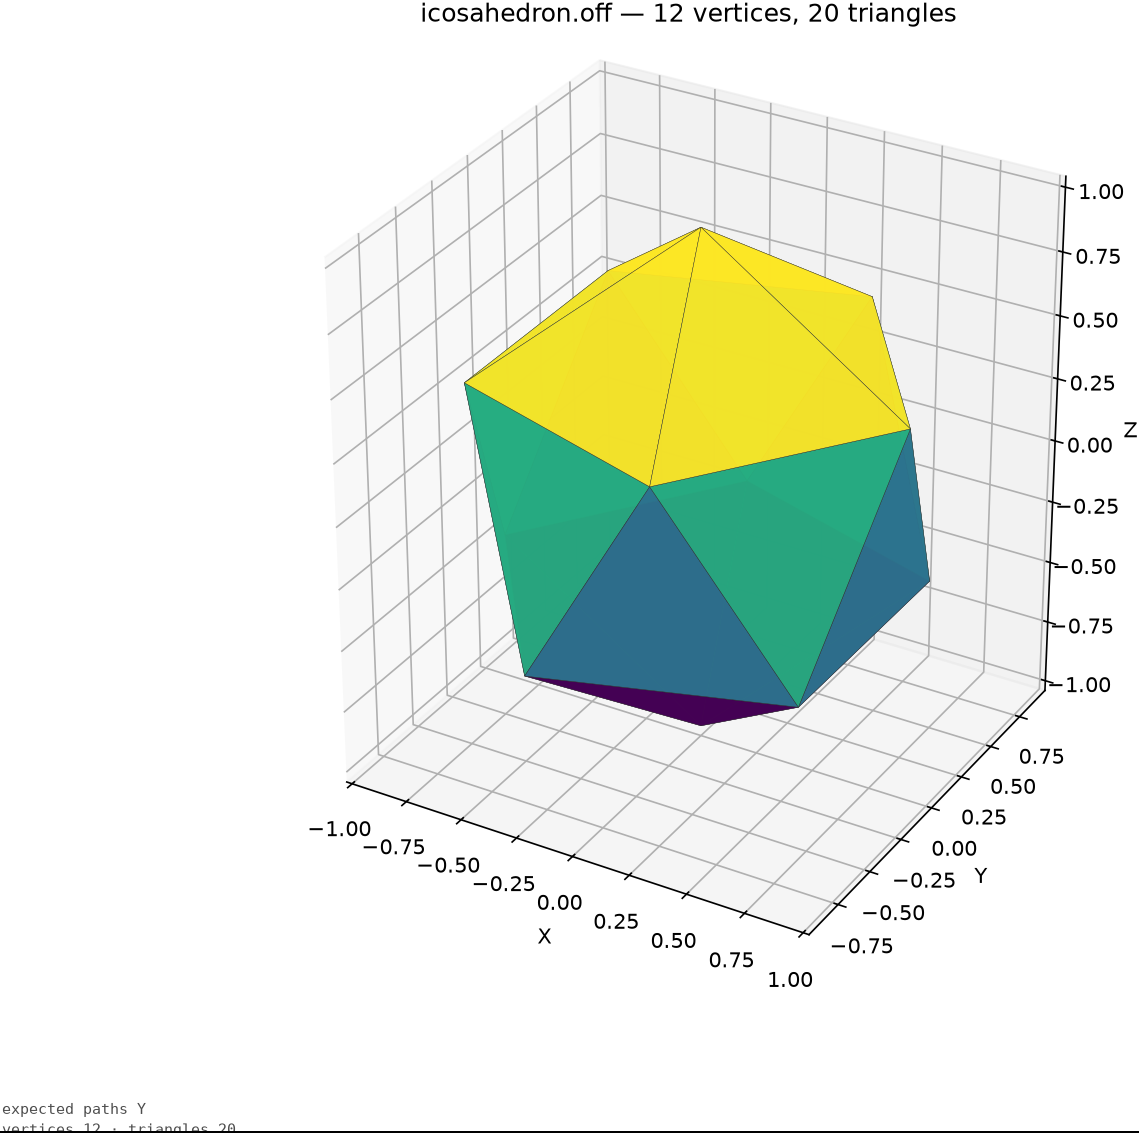
\includegraphics[width=\linewidth]{Figures/crop/repo_icosahedron.png}
    \caption{\texttt{icosahedron} ($V=12$, $F=20$)}
  \end{subfigure}\hfill
  \begin{subfigure}{0.46\textwidth}
    \centering
    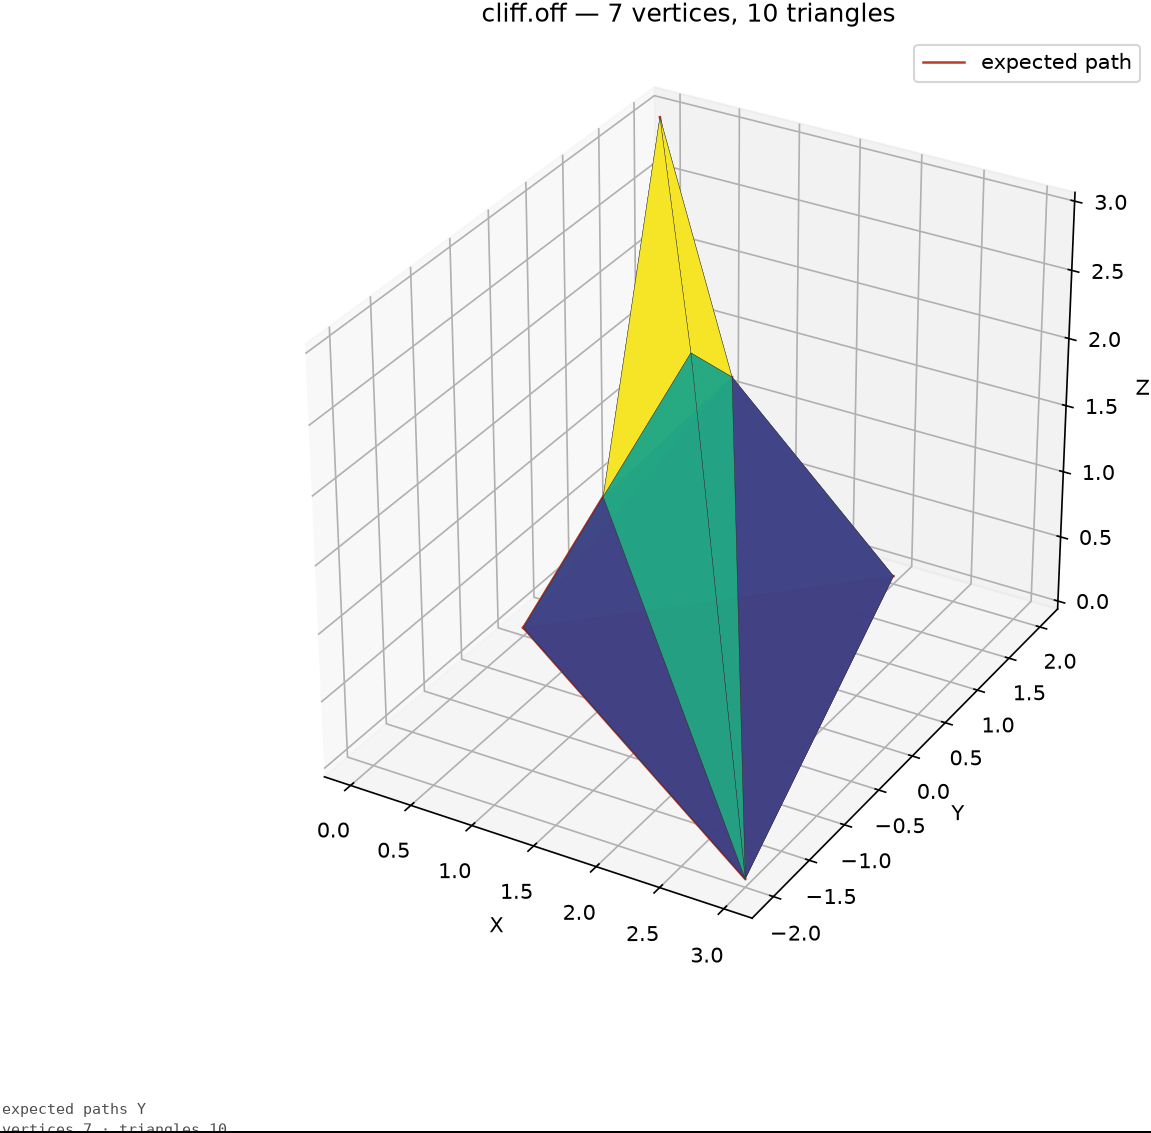
\includegraphics[width=\linewidth]{Figures/crop/repo_cliff.png}
    \caption{\texttt{cliff} ($V=7$, $F=10$)}
  \end{subfigure}\par\vspace{2pt}
  \begin{subfigure}{0.46\textwidth}
    \centering
    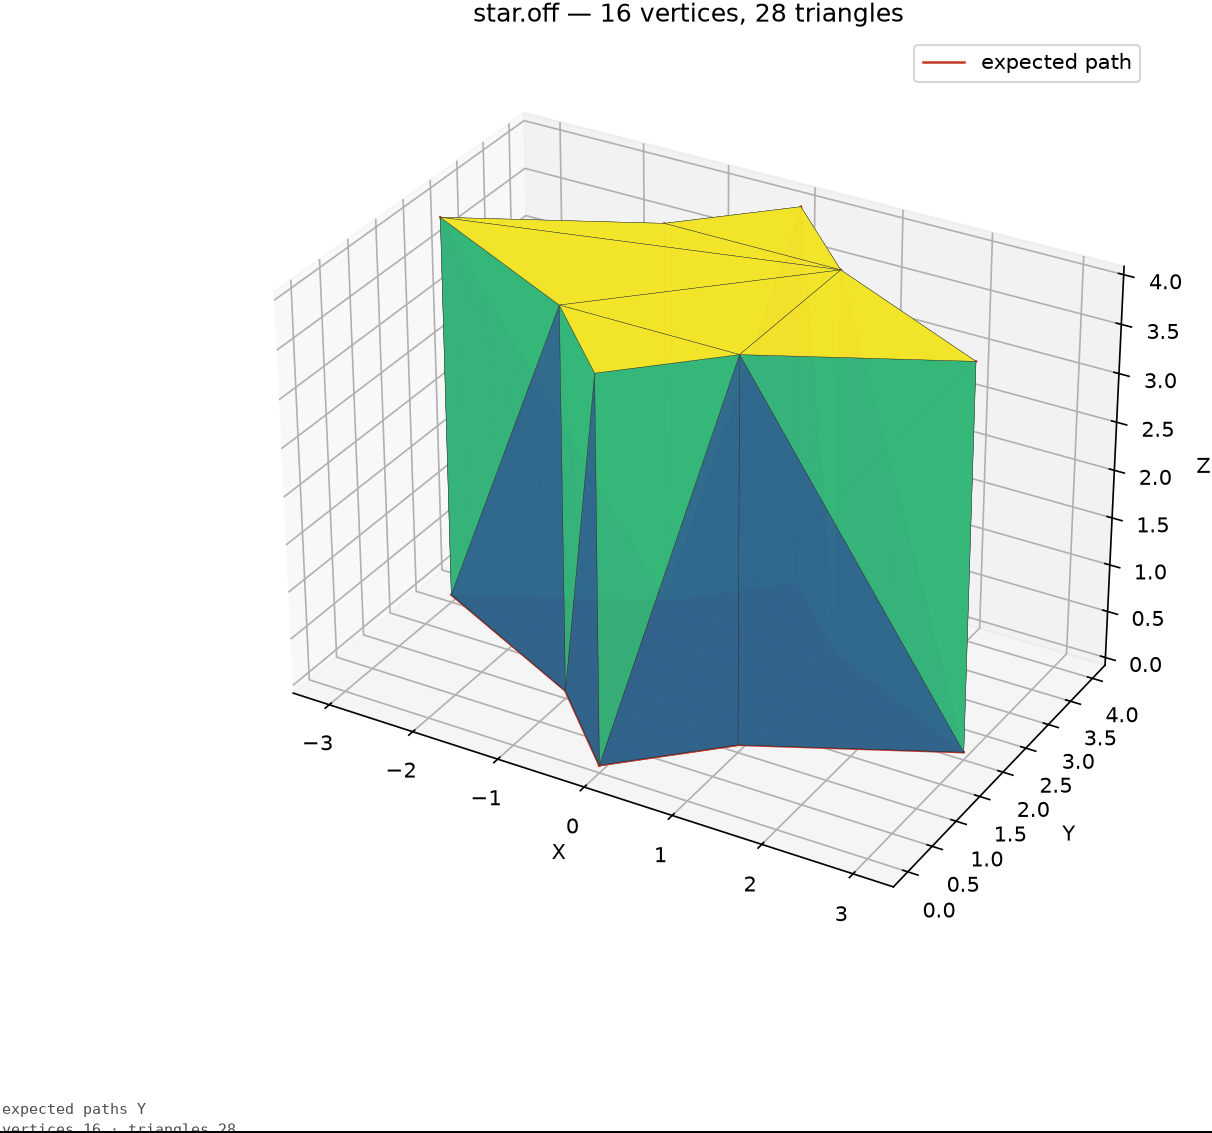
\includegraphics[width=\linewidth]{Figures/crop/repo_star.png}
    \caption{\texttt{star} ($V=16$, $F=28$)}
  \end{subfigure}
  \caption{Trực quan hóa một số lưới đa diện bề mặt kín tiêu biểu, kết xuất từ
    công cụ trực quan hóa.}
  \label{fig:closed-meshes}
\end{figure*}

Hình~\ref{fig:closed-meshes} cho thấy ba dạng hình học rất khác nhau: khối
icosahedron lồi đều với các mặt tam giác, \texttt{cliff} có một vách dốc và các
sườn nghiêng, còn \texttt{star} lõm với các múi nhọn. Sự khác biệt này là cơ sở
để kiểm tra thuật toán trên cả bề mặt lồi và không lồi.

Hình~\ref{fig:closed-meshes-2} tiếp tục trực quan hóa ba mô hình bề mặt kín còn
lại của bộ dữ liệu: khối lập phương \texttt{cube}, và hai mesh có dữ liệu đối
chiếu chuẩn là \texttt{J17} và \texttt{L}. Như vậy,
cả bảy mesh bề mặt kín đều được thể hiện trực quan đầy đủ.

\begin{figure*}[!t]
  \centering
  \begin{subfigure}{0.46\textwidth}
    \centering
    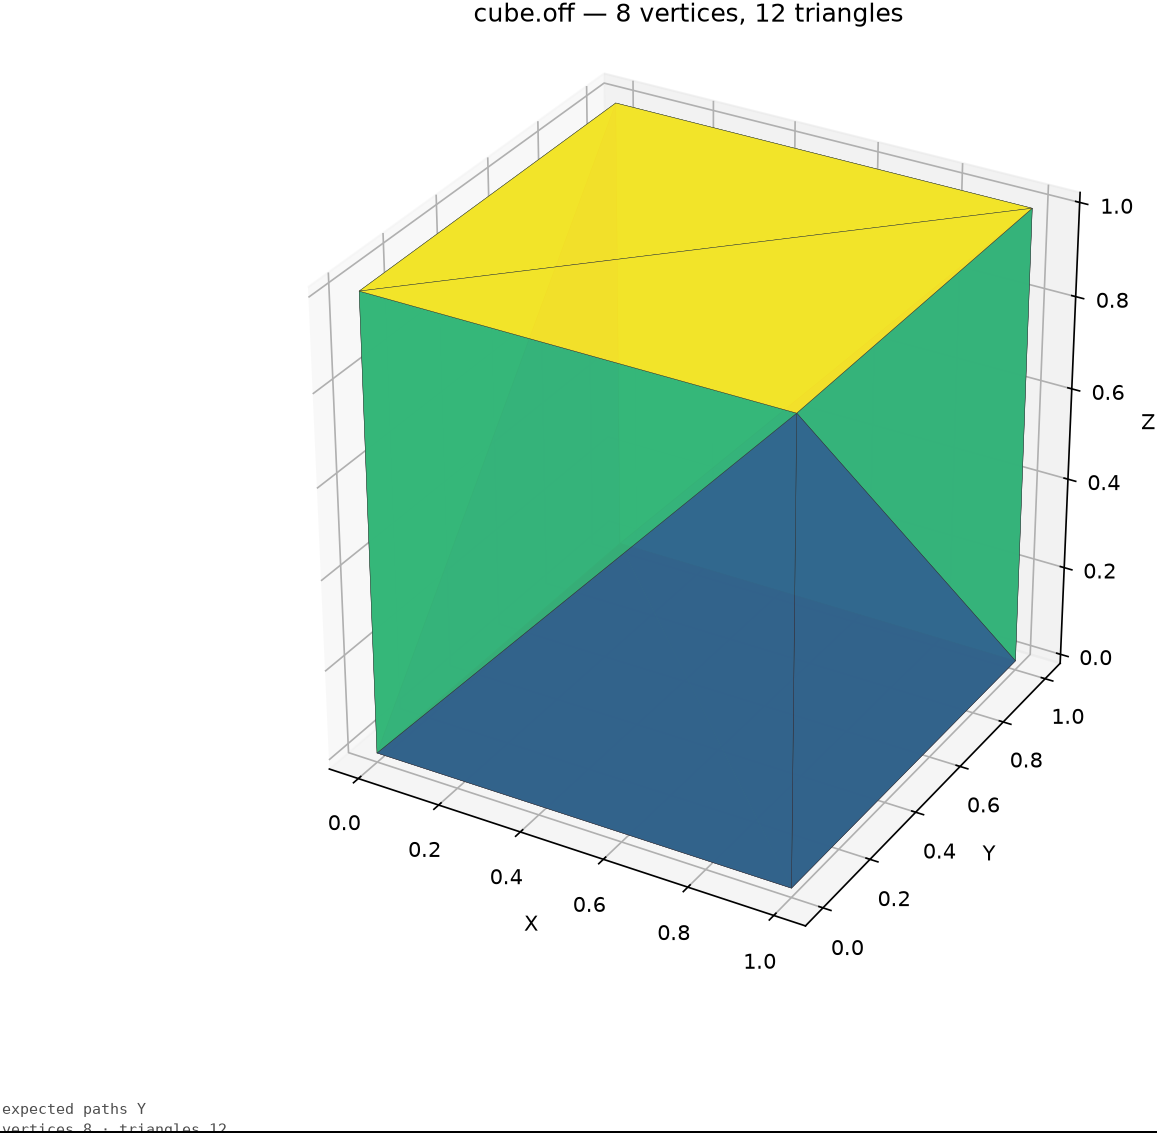
\includegraphics[width=\linewidth]{Figures/crop/repo_cube.png}
    \caption{\texttt{cube} ($V=8$, $F=12$, $s=4$)}
  \end{subfigure}\hfill
  \begin{subfigure}{0.46\textwidth}
    \centering
    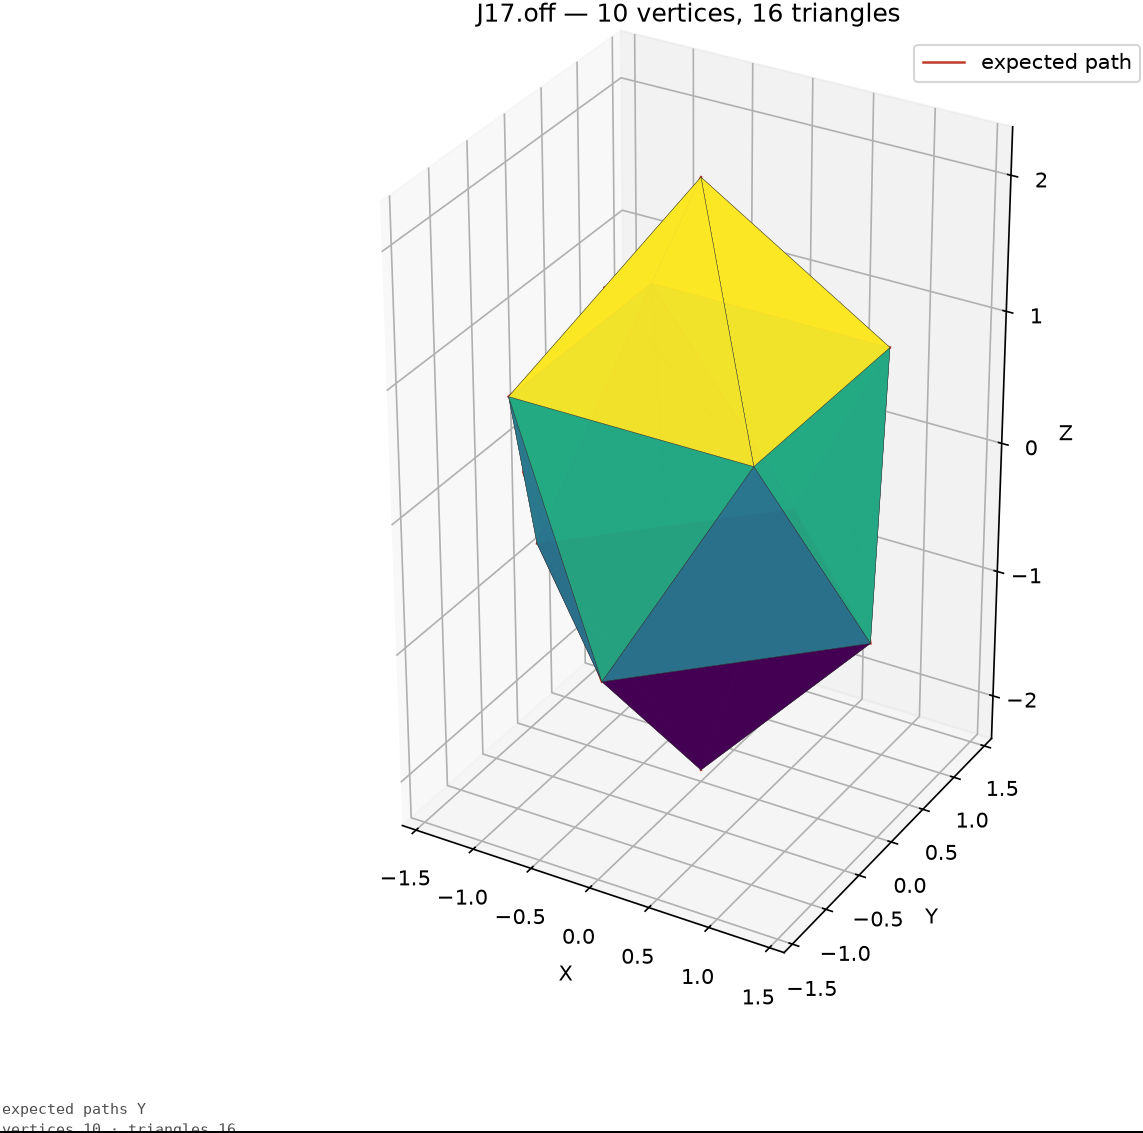
\includegraphics[width=\linewidth]{Figures/crop/repo_J17.png}
    \caption{\texttt{J17} ($V=10$, $F=16$, $s=1$)}
  \end{subfigure}\par\vspace{2pt}
  \begin{subfigure}{0.46\textwidth}
    \centering
    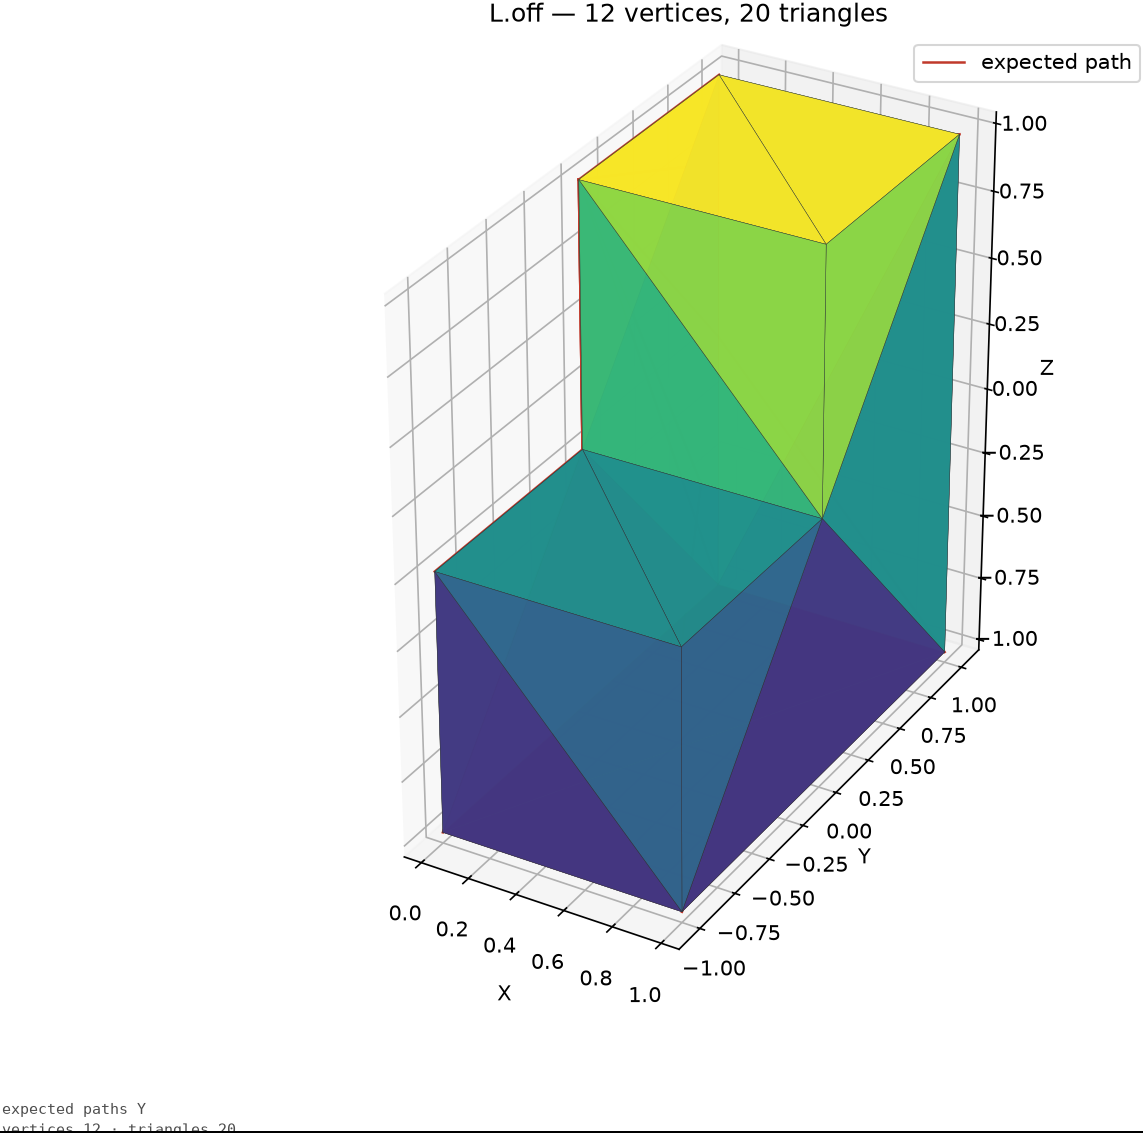
\includegraphics[width=\linewidth]{Figures/crop/repo_L.png}
    \caption{\texttt{L} ($V=12$, $F=20$, $s=1$)}
  \end{subfigure}
  \caption{Trực quan hóa ba mô hình bề mặt kín còn lại trong bộ dữ liệu, kết xuất
    từ công cụ trực quan hóa.}
  \label{fig:closed-meshes-2}
\end{figure*}

Hình~\ref{fig:closed-meshes-2} cho thấy \texttt{cube} là khối lồi đơn giản,
\texttt{J17} và \texttt{L} có các mặt phẳng nghiêng nối với nhau; cả ba đều có
đường tham chiếu đi qua mặt, không chỉ qua cạnh. Đây là các ca thuận lợi để kiểm
tra độ dài trước khi chuyển sang bề mặt phức tạp hơn.

Hình~\ref{fig:view-layers} minh họa hai lớp thông tin mà quy trình đối chiếu dùng
cho mesh \texttt{J17}: panel trái là đường tham chiếu phủ lên mesh; panel phải là
tập route do công cụ vẽ tuyến sinh, tức kết quả của Funnel Tree cho mọi đỉnh
đích. Hai panel dùng cùng dữ liệu đầu vào nhưng khác nguồn đường, nhờ đó có
thể so trực tiếp bằng mắt trước khi so độ dài ở Mục~\ref{sec:results}.

\begin{figure*}[!t]
  \centering
  \begin{subfigure}{0.46\textwidth}
    \centering
    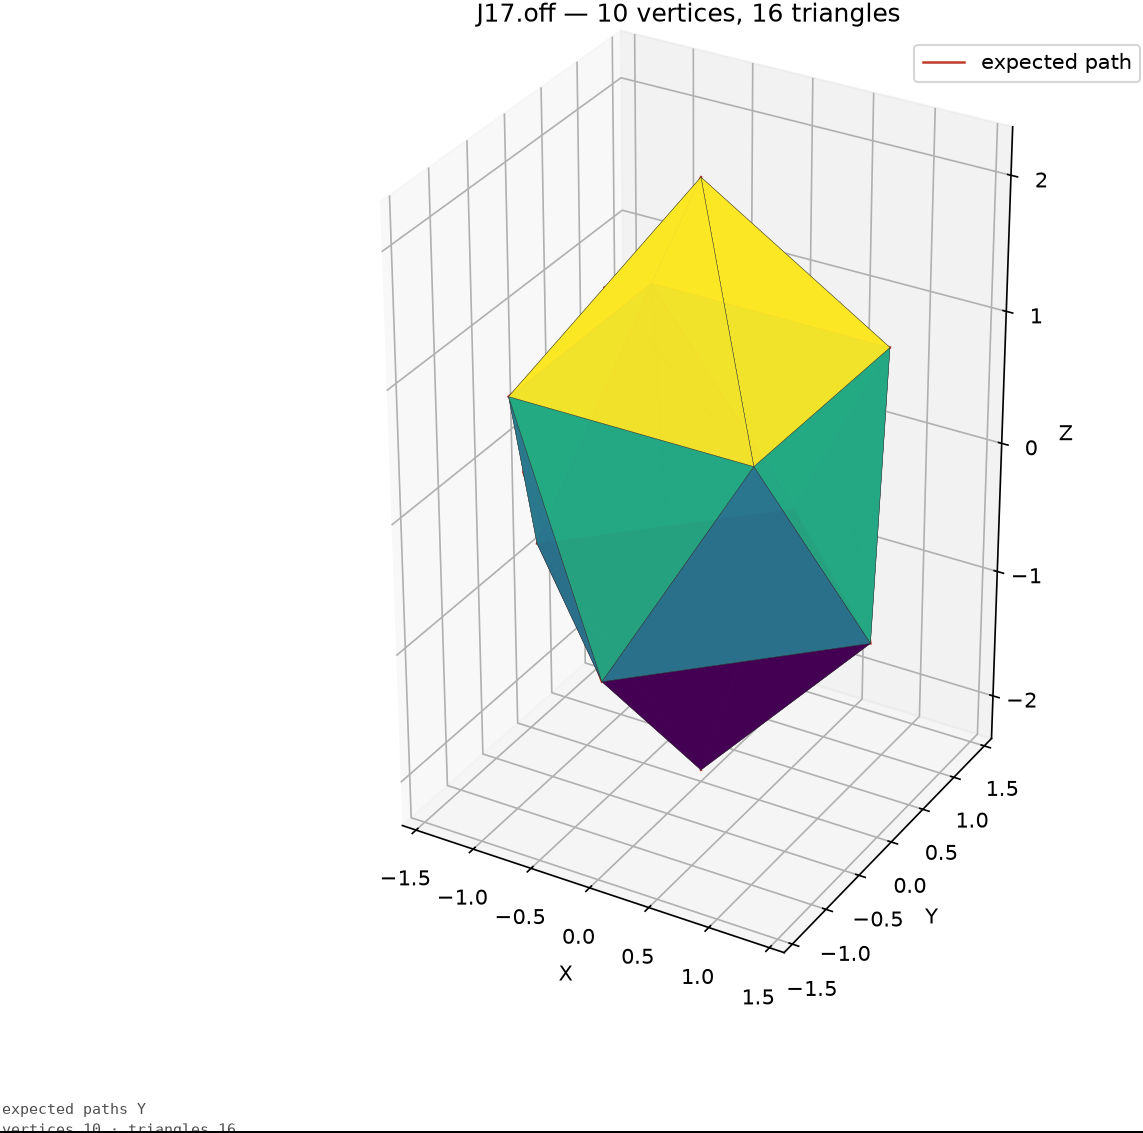
\includegraphics[width=\linewidth]{Figures/crop/repo_J17.png}
    \caption{Đường tham chiếu độc lập.}
  \end{subfigure}\hfill
  \begin{subfigure}{0.46\textwidth}
    \centering
    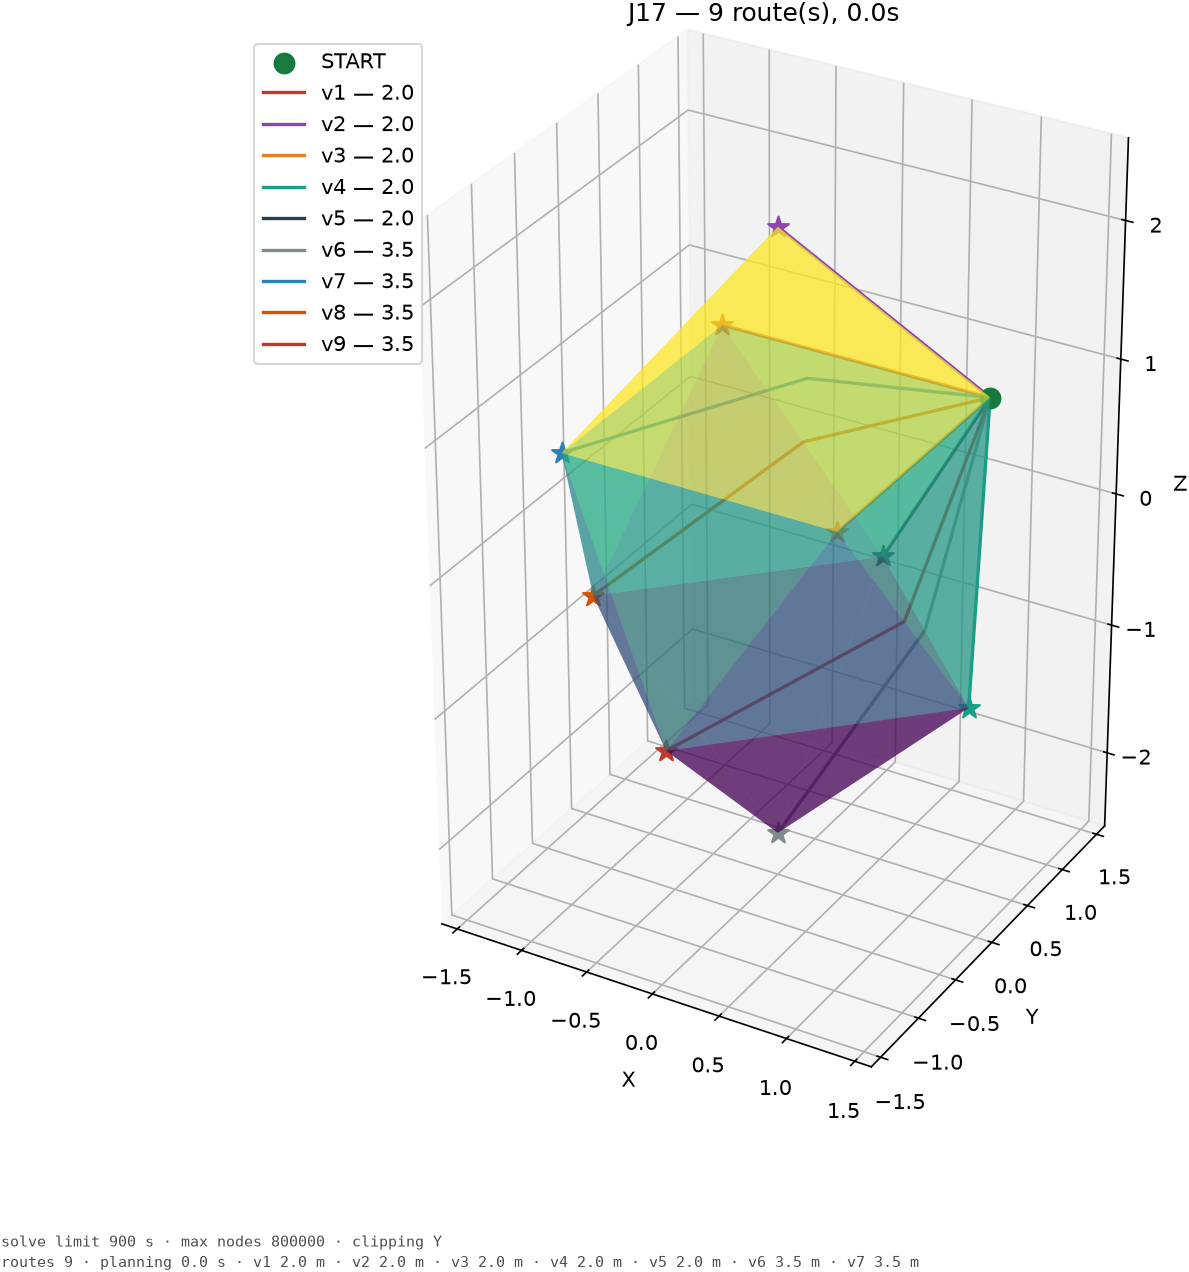
\includegraphics[width=\linewidth]{Figures/crop/repo_J17_routes.png}
    \caption{Route do Funnel Tree trả về.}
  \end{subfigure}
  \caption{Hai lớp hiển thị trên mesh \texttt{J17}: dữ liệu tham chiếu (trái) và
    kết quả Funnel Tree cho mọi đỉnh đích (phải). Cả hai ảnh đều có chân ghi
    tham số và SHA.}
  \label{fig:view-layers}
\end{figure*}

Hình~\ref{fig:open-meshes} cho thấy \texttt{dome} là một mảnh vỏ cầu khuyết
đáy còn \texttt{terrain} là mặt địa hình có thung lũng; cả hai đều có chu vi biên
hở. Các đường tham chiếu dừng ở biên thay vì đi xuyên qua, đúng ràng buộc mà thuật
toán phải xử lý.

Đối với bài toán mở rộng bề mặt mở, Hình~\ref{fig:open-meshes} trực quan hóa hai
mô hình bề mặt mở: vỏ cầu khuyết đáy \texttt{dome} và mô hình địa hình đồi núi
\texttt{terrain}. Trên các hình ảnh này, đường biên hở bao quanh mô hình thể hiện
rõ giới hạn không gian mà các tia tìm kiếm funnel không được phép vượt qua.

\begin{figure*}[!t]
  \centering
  \begin{subfigure}{0.45\textwidth}
    \centering
    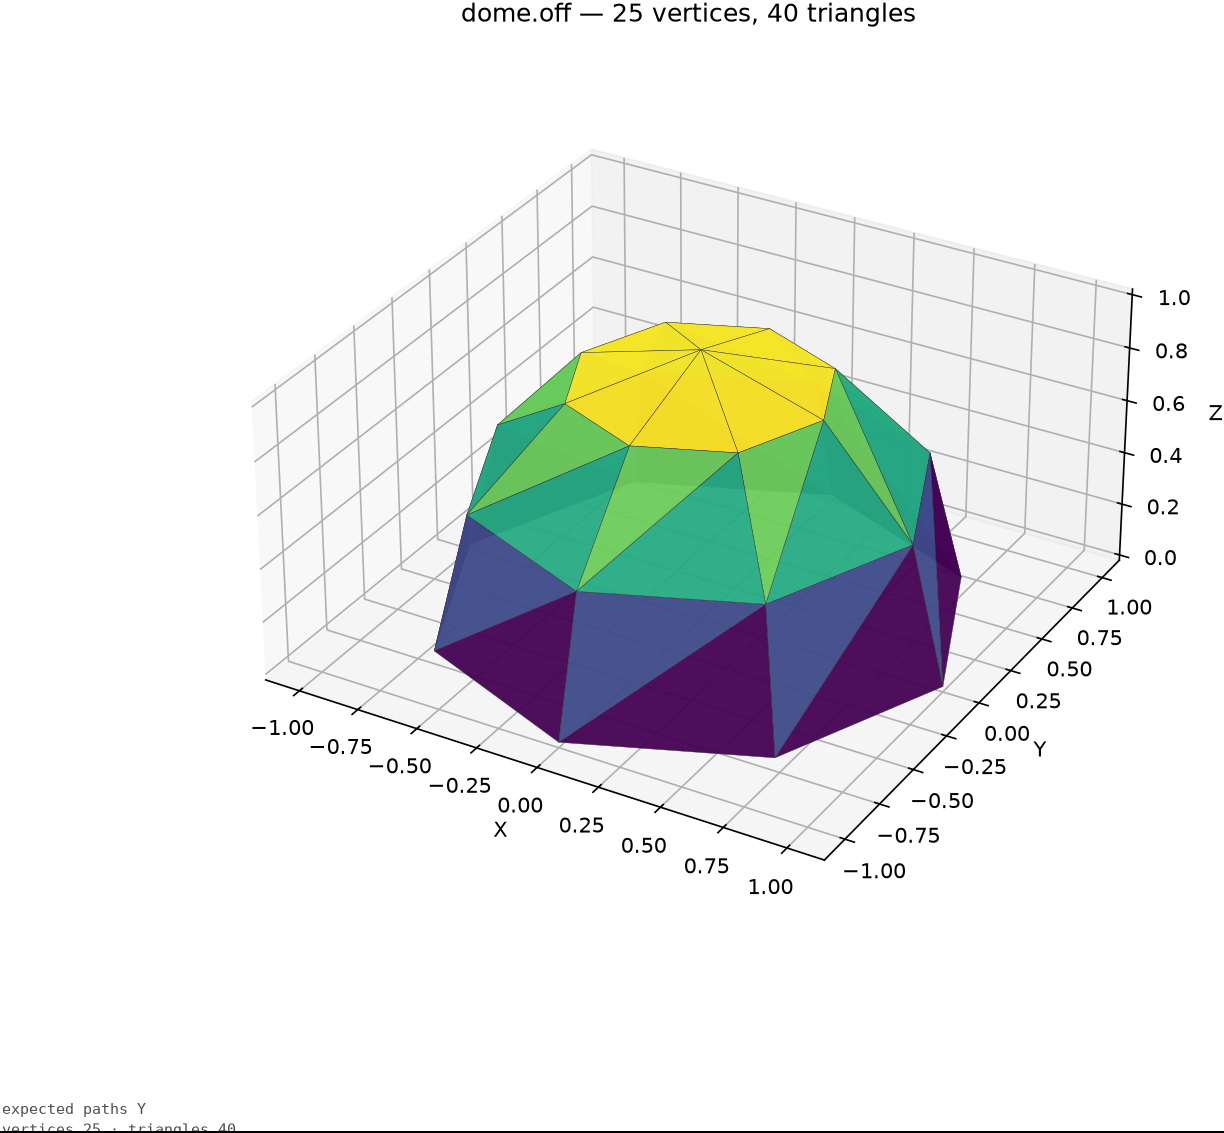
\includegraphics[width=\linewidth]{Figures/crop/repo_dome.png}
    \caption{\texttt{dome} ($V=25$, $F=40$, 8 cạnh biên)}
  \end{subfigure}\hfill
  \begin{subfigure}{0.45\textwidth}
    \centering
    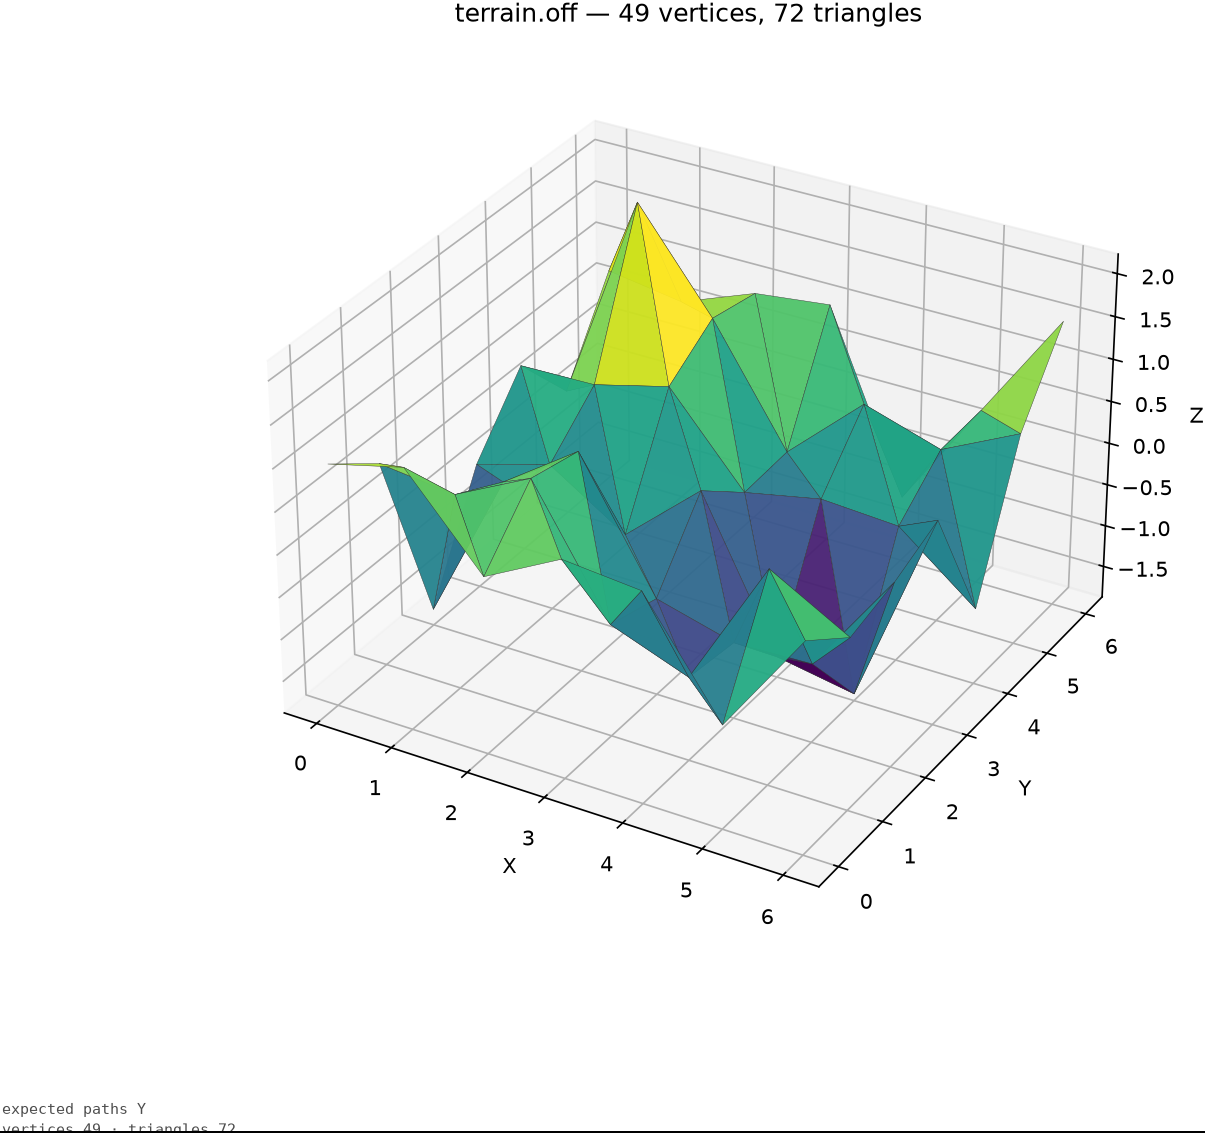
\includegraphics[width=\linewidth]{Figures/crop/repo_terrain.png}
    \caption{\texttt{terrain} ($V=49$, $F=72$, 24 cạnh biên)}
  \end{subfigure}
  \caption{Trực quan hóa hai mô hình bề mặt mở có cạnh biên, kết xuất từ
    công cụ trực quan hóa.}
  \label{fig:open-meshes}
\end{figure*}

Cuối cùng, Hình~\ref{fig:demo-mesh} biểu diễn mô hình \texttt{demo\_mesh} --- mesh
có số đỉnh và số mặt lớn nhất trong nhóm bề mặt kín, sở hữu cấu trúc tô pô dạng
xuyến ($\chi=0$) với lỗ rỗng ở trung tâm và thang đo tọa độ lớn hơn 100 lần.

\begin{figure}[!t]
  \centering
  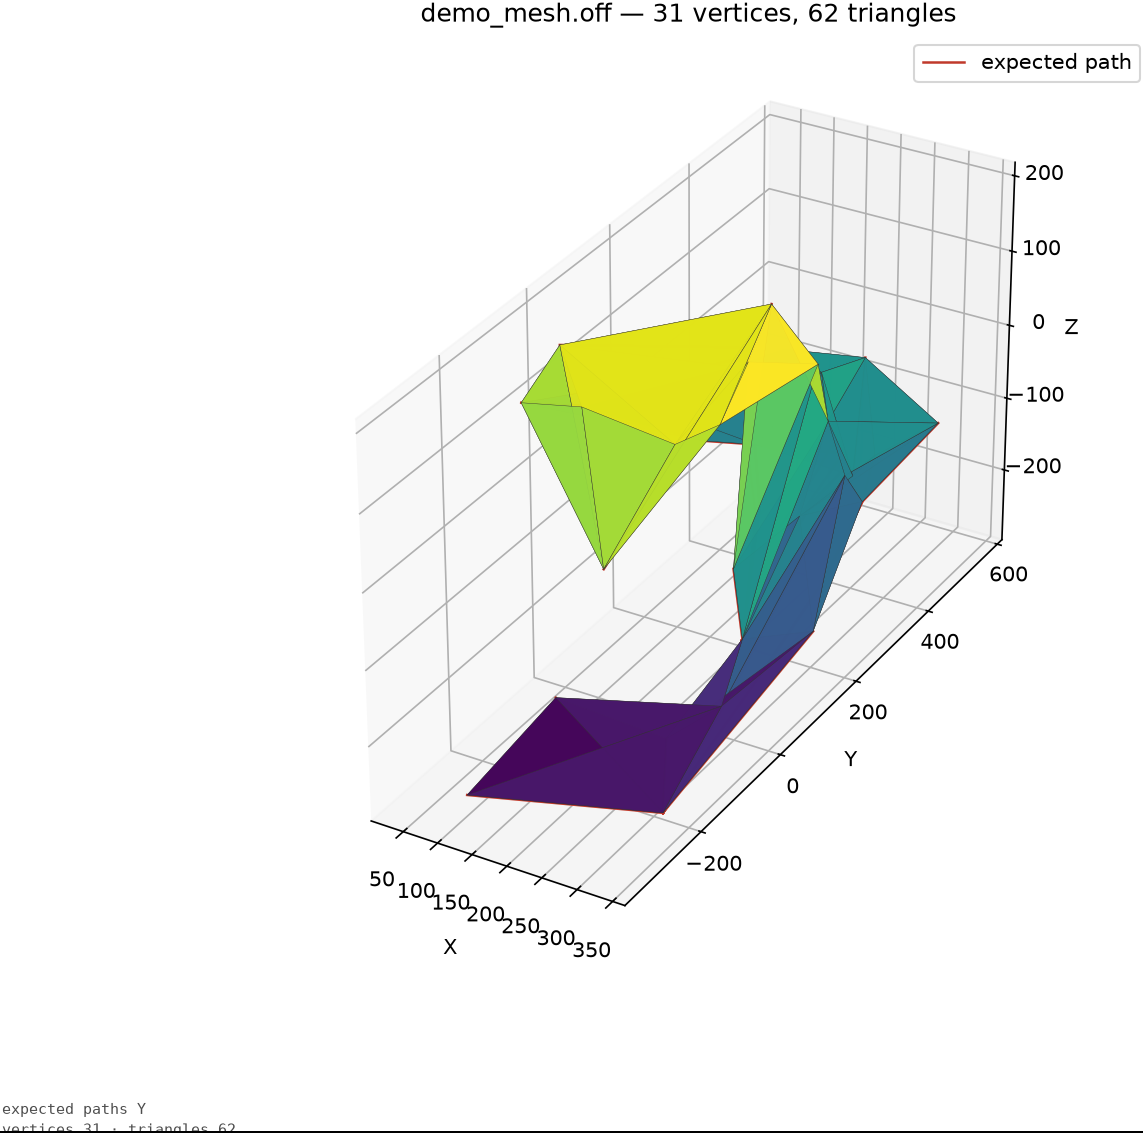
\includegraphics[width=0.95\linewidth]{Figures/crop/repo_demo_mesh.png}
  \caption{Mô hình \texttt{demo\_mesh} ($V=31$, $F=62$, $\chi=0$) dạng xuyến,
    kết xuất bởi công cụ trực quan hóa; đường tham chiếu được phủ lên mesh.}
  \label{fig:demo-mesh}
\end{figure}

Hình~\ref{fig:demo-mesh} cho thấy \texttt{demo\_mesh} có lỗ xuyên tâm và thang
tọa độ lớn hơn các mesh khác khoảng 100 lần; các đường tham chiếu vòng qua lỗ và
giữ được hình dạng xuyến. Đây là ca kiểm tra tính đúng trên bề mặt có lỗ và là lý
do mọi so sánh sai số phải dùng đại lượng tương đối.

\subsection{Insights từ EDA}

Từ các kết quả EDA và trực quan hóa dữ liệu ở trên, nghiên cứu rút ra năm insight
quan trọng, định hình trực tiếp phương pháp đánh giá thực nghiệm:
\begin{enumerate}
  \item \textbf{Dữ liệu kiểm chứng bề mặt mở đã sẵn sàng:} với sự hiện diện của
    \texttt{dome.off} (8 cạnh biên) và \texttt{terrain.off} (24 cạnh biên), kho
    mã nguồn \cite{kien2026repo} đã cung cấp đầy đủ dữ liệu để kiểm chứng thuật
    toán trên bề mặt mở (mục tiêu~3). Việc trực quan hóa ở
    Hình~\ref{fig:open-meshes} xác nhận rõ các đường biên không gian cần được xử
    lý cắt tỉa biên trong thuật toán.
  \item \textbf{Độ phong phú về dạng hình học nhưng quy mô còn nhỏ so với bài
    báo:} dữ liệu kiểm thử đã bao quát từ đa diện lồi, không lồi, dạng xuyến đến
    bề mặt mở, nhưng kích thước tối đa mới đạt $V=49$ đỉnh (so với 100--800 đỉnh ở
    \cite{an2024funnel}). Do đó, các thí nghiệm ở Mục~\ref{sec:results} đóng vai
    trò kiểm chứng tính đúng đắn và độ ổn định thuật toán, chưa phải là phép đo
    hiệu năng trên dữ liệu lớn.
  \item \textbf{Khác biệt thang đo khoảng 100 lần giữa \texttt{demo\_mesh} và các
    mesh khác:} mọi so sánh sai số ở Mục~\ref{sec:results} bắt buộc phải dùng sai
    số tương đối, không dùng sai số tuyệt đối khi đánh giá gộp các mô hình.
  \item \textbf{Độ tin cậy của output tham chiếu:} 5/9 mesh có file tham chiếu
    tham chiếu; bước đối chiếu so 76 đỉnh với
    ngưỡng tương đối $10^{-4}$ và hiện báo 0 failure. Bốn mesh còn lại không có
    tham chiếu độc lập, nên chỉ dùng để kiểm tra khả năng chạy trên bề mặt lồi,
    bề mặt mở và bề mặt có lỗ.
  \item \textbf{Mô hình thành phố \texttt{city.glb} là tiền đề cho bài toán đô thị
    thực tế:} file \texttt{city.glb} (khoảng 20,5 MB) nằm trong
    dữ liệu gốc. File này được đưa vào tính toán ở phần mô phỏng
    (Mục~\ref{sec:gazebo}), nơi mô hình thành phố được chuyển thành bề mặt dẫn
    đường tam giác hóa để lập tuyến cho UAV.
\end{enumerate}

%% ---------------------------------------------------------------------
%% 04 - KẾT QUẢ VÀ THẢO LUẬN
%% ---------------------------------------------------------------------

\section{Kết quả và thảo luận}\label{sec:results}

Mục này trình bày kết quả thực nghiệm của thuật toán Funnel Tree kết hợp Thủ tục 2
(\emph{Clip off Funnels}) được cài đặt bằng Python, đối sánh với chương trình
tham chiếu trên 5 mesh nhỏ và phân tích trường hợp điển hình trên lưới địa hình
vách dốc. Trọng tâm gồm: (1) đánh giá tổng thể trên 9 mesh kiểm thử; (2) phân
tích chuyên sâu lưới \texttt{cliff} kèm trực quan hóa; (3) mô tả cơ chế cắt tỉa
trong cài đặt hiện tại; (4) phân tích sai số và thảo luận ý nghĩa ứng dụng.

\subsection{Kết quả thực nghiệm tổng thể trên các lưới đa diện}

Thuật toán được thực thi trên 9 mesh \texttt{.off} của bộ dữ liệu. Kết quả được đối soát theo ba tiêu chí:
\begin{description}
  \item[Độ sai lệch so với chương trình tham chiếu]
    ($|L_{\text{Funnel}}-L_{\text{ref}}|/L_{\text{ref}}$): so sánh độ dài polyline
    đến từng đỉnh với đường tham chiếu độc lập; reference được làm tròn 4 chữ số
    thập phân.
  \item[Khả năng chạy và tính nhất quán nội tại] với 4 mesh không có reference,
    kiểm tra route được dựng cho mọi đỉnh đích và độ dài polyline dựng lại khớp
    độ dài nội tại mà phép lan truyền tính được.
  \item[Quy mô tìm kiếm] ghi nhận số lần lan truyền và việc bật/tắt cắt tỉa trong
    route JSON, thay cho số nút cây và số sự kiện clip mà phiên bản cũ ghi riêng.
\end{description}
Bảng~\ref{tab:ket-qua-tong-the} tổng hợp các chỉ số thu được.

\begin{table*}[!t]
  \caption{Kết quả chạy Funnel Tree trên 9 lưới đa diện. $P$ là số lần lan truyền;
    sai số tương đối chỉ tính cho 5 mesh có file tham chiếu. Dấu ``---'' nghĩa là
    không có reference độc lập.}
  \label{tab:ket-qua-tong-the}
  {\fontsize{7}{8.6}\selectfont
  \begin{adjustbox}{max width=\textwidth}
  \begin{tabular}{@{}lrrrrrrl@{}}
    \toprule
    \textbf{Lưới đa diện} & $V$ & $F$ & \textbf{Nguồn $s$} & $P$
      & \textbf{Sai số tương đối lớn nhất} & \textbf{Trung bình} & \textbf{Reference} \\
    \midrule
    \texttt{cliff}       &  7 & 10  & 1 &  3 & $1{,}7\times10^{-5}$ & $2{,}6\times10^{-6}$ & Có \\
    \texttt{cube}        &  8 & 12  & 0 &  1 & --- & --- & Không \\
    \texttt{J17}         & 10 & 16  & 1 &  1 & $4{,}8\times10^{-6}$ & $1{,}7\times10^{-6}$ & Có \\
    \texttt{L}           & 12 & 20  & 1 &  3 & $9{,}0\times10^{-10}$ & $7{,}5\times10^{-11}$ & Có \\
    \texttt{icosahedron} & 12 & 20  & 0 &  1 & --- & --- & Không \\
    \texttt{star}        & 16 & 28  & 0 &  9 & $6{,}7\times10^{-6}$ & $8{,}3\times10^{-7}$ & Có \\
    \texttt{dome}        & 25 & 40  & 0 &  1 & --- & --- & Không \\
    \texttt{demo\_mesh}  & 31 & 62  & 1 & 20 & $3{,}6\times10^{-7}$ & $8{,}5\times10^{-8}$ & Có \\
    \texttt{terrain}     & 49 & 72  & 0 & 26 & --- & --- & Không \\
    \bottomrule
  \end{tabular}
  \end{adjustbox}}
  \par\smallskip
  {\footnotesize $P$ lấy từ \texttt{stats.propagations} của route JSON; sai số
  tương đối lấy từ kết quả đối chiếu. Mọi lần chạy đều bật cắt tỉa.}
\end{table*}

Nhận xét tổng quan:
\begin{itemize}
  \item Trên 5/5 lưới có dữ liệu đối chiếu chuẩn (\texttt{cliff}, \texttt{J17},
    \texttt{L}, \texttt{star}, \texttt{demo\_mesh}), tổng cộng 76 đỉnh được so,
    không có failure ở ngưỡng tương đối $10^{-4}$. Sai số tương đối lớn nhất là
    $1{,}7\times10^{-5}$ (\texttt{cliff}), phát sinh từ việc reference chỉ giữ
    bốn chữ số thập phân; các mesh còn lại có sai số nhỏ hơn một bậc.
  \item Bốn mesh không có reference (\texttt{cube}, \texttt{icosahedron},
    \texttt{dome}, \texttt{terrain}) vẫn dựng được route cho mọi đỉnh đích, với
    $P=1$, $1$, $1$ và $26$. Đây là kiểm tra khả năng chạy trên bề mặt lồi, bề mặt
    mở và bề mặt có lỗ, không phải đối chiếu độ dài với một bộ giải thứ hai.
  \item Mọi route JSON ghi \texttt{clipping=true}; cài đặt hiện tại không phát
    sinh log từng sự kiện clip, nên bài báo không báo số lần cắt cụt cụ thể. Cơ
    chế cắt tỉa được mô tả định tính ở Mục~\ref{sec:clip}.
\end{itemize}

\begin{code}[!t]
  \lstinputlisting[style=jsoncode]{Code/compare_excerpt.json}
  \caption{Trích kết quả đối chiếu của \texttt{cliff}: thông tin mesh,
    nguồn, dung sai, sai số tương đối và danh sách độ dài từng đỉnh. Trường
    \texttt{paths} là nguồn của Bảng~\ref{tab:ket-qua-tong-the} và
    Bảng~\ref{tab:cliff-output}.}
  \label{code:compare}
\end{code}

\subsection{Nghiên cứu trường hợp điển hình: địa hình vách dốc}

Để làm rõ cơ chế vận hành từ khâu đọc dữ liệu hình học, dựng cây đến truy hồi
polyline, nghiên cứu phân tích chi tiết lưới \texttt{cliff} ($V=7$, $F=10$,
$E=15$). Đây là mô hình tiêu biểu cho địa hình đô thị hiểm trở với các sườn nghiêng
và vách đá dốc đứng.

\subsubsection{Mô hình bài toán và dữ liệu đầu vào}

Bài toán đặt trong bối cảnh: trạm chỉ huy và tiếp vận UAV đặt tại chân vách đá
$s=1$ tọa độ $(0,0,0)$. UAV cần vận chuyển hàng cứu trợ khẩn cấp lên điểm cao nhất
tại đỉnh vách đá $v=6$ tọa độ $(0,2,3)$, đồng thời thiết lập các tuyến đường tối ưu
đến toàn bộ các mốc quan trắc trung gian $v\in\{0,2,3,4,5\}$.

Dữ liệu đầu vào chuẩn \texttt{cliff.off} được biểu diễn như sau:
\begin{itemize}
  \item Dòng tiêu đề xác định kích thước hình học: $V=7$ đỉnh, $F=10$ mặt tam giác,
    $E=15$ cạnh.
  \item Tọa độ 7 đỉnh trong không gian $\R^3$: $v_0(2;2;0)$, $v_1(0;0;0)$ (nguồn
    $s$), $v_2(3;-2;0)$, $v_3(2;-1;3)$, $v_4(1;-0{,}5;1{,}5)$,
    $v_5(0{,}91865;1{,}45943;1{,}5)$ và $v_6(0;2;3)$ (đỉnh vách).
  \item Danh sách 10 mặt tam giác được định nghĩa bởi bộ ba chỉ số đỉnh:
    $f_0(0,1,5)$, $f_1(1,4,5)$, $f_2(3,5,6)$, $f_3(3,4,6)$, $f_4(4,5,6)$,
    $f_5(1,2,4)$, $f_6(2,3,4)$, $f_7(2,0,5)$, $f_8(2,3,5)$ và $f_9(1,0,2)$.
\end{itemize}

\subsubsection{Trực quan hóa không gian ba chiều}

Hình~\ref{fig:cliff-visual} minh họa kết quả không gian 3D do
công cụ trực quan hóa kết xuất, thể hiện cấu trúc lưới tam giác và các
đường tham chiếu tỏa ra từ đỉnh nguồn $s=1$.

\begin{figure}[!t]
  \centering
  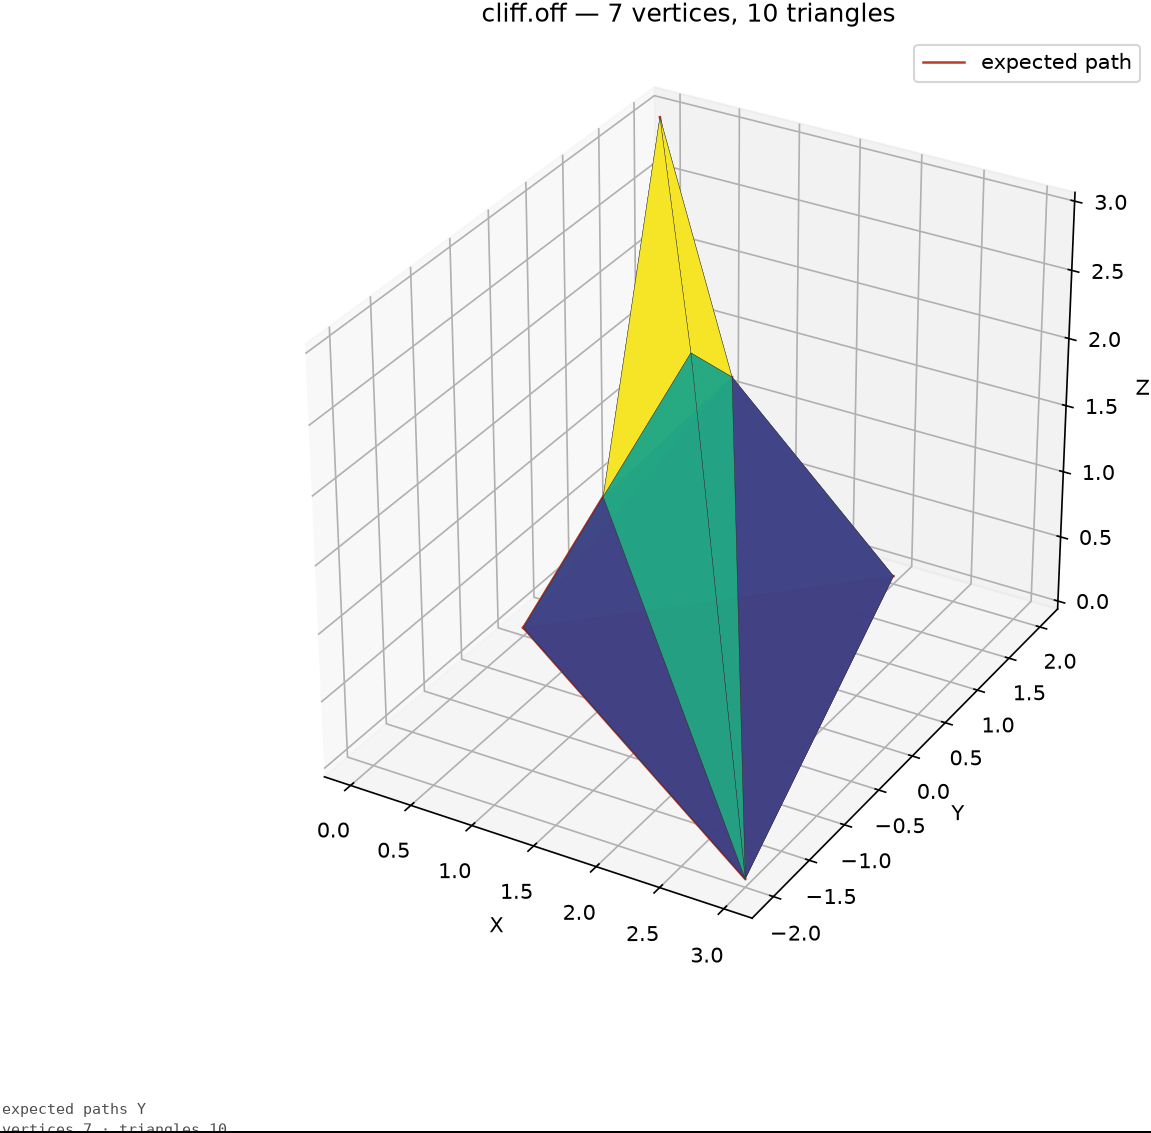
\includegraphics[width=0.95\linewidth]{Figures/crop/repo_cliff.png}
  \caption{Trực quan hóa đường tham chiếu trên bề mặt địa hình \texttt{cliff}
    với đỉnh nguồn $s=1$, kết xuất bởi công cụ trực quan hóa. Các đường màu đỏ là
    polyline tham chiếu; độ dài do
    Funnel Tree tính được đối chiếu ở Bảng~\ref{tab:cliff-output}.}
  \label{fig:cliff-visual}
\end{figure}

Từ Hình~\ref{fig:cliff-visual}, hai đặc trưng hình học quan trọng được làm sáng tỏ:
\begin{enumerate}
  \item Các polyline tham chiếu được vẽ trên cùng một mesh; độ dài do Funnel Tree trả về được đối chiếu với
    chúng ở Bảng~\ref{tab:cliff-output}. Ảnh không chồng hai lớp đường, nên việc
    so khớp được thực hiện bằng số liệu chứ không bằng mắt.
  \item Tuyến đường từ trạm $s=1$ lên đỉnh cao nhất $v=6$ cắt ngang qua cạnh
    $[4,5]$ tại điểm nội tại $(0,9356;1,0513;1,5000)$ --- đây là ưu thế của Funnel
    Tree so với xấp xỉ qua đỉnh của đồ thị rời rạc.
\end{enumerate}

\subsubsection{Dữ liệu đầu ra và phân tích polyline}

Bảng~\ref{tab:cliff-output} phân tích chi tiết polyline kết quả cho lưới
\texttt{cliff}, đối chiếu giữa đường tham chiếu trong
đường tham chiếu và độ dài do Funnel Tree trả về trong kết quả đối chiếu.

\begin{table*}[!t]
  \caption{Chi tiết polyline đường đi ngắn nhất từ nguồn $s=1$ trên lưới
    \texttt{cliff}.}
  \label{tab:cliff-output}
  {\fontsize{7}{8.6}\selectfont
  \begin{tabular}{@{}rr>{\raggedright\arraybackslash}p{150pt}r>{\raggedright\arraybackslash}p{118pt}@{}}
    \toprule
    \textbf{Đích $v$} & \textbf{Số điểm $m$} & \textbf{Tọa độ các điểm trên
      polyline} & \textbf{Chiều dài} & \textbf{Đặc điểm hình học} \\
    \midrule
    $0$ & 2 & $[0;0;0]\to[2;2;0]$ & 2,8284 & Đoạn thẳng trên mặt phẳng đáy
      $\triangle 102$ \\
    $1$ & 2 & $[0;0;0]\to[0;0;0]$ & 0,0000 & Đỉnh nguồn $s=1$ (phân đoạn suy
      biến) \\
    $2$ & 2 & $[0;0;0]\to[3;-2;0]$ & 3,6056 & Đoạn thẳng trên mặt phẳng đáy
      $\triangle 102$ \\
    $3$ & 3 & $[0;0;0]\to[1;-0{,}5;1{,}5]\to[2;-1;3]$ & 3,7417 & Gãy góc qua đỉnh gờ
      trung gian $v=4$ \\
    $4$ & 2 & $[0;0;0]\to[1;-0{,}5;1{,}5]$ & 1,8708 & Đoạn thẳng trực tiếp trên mặt
      sườn $\triangle 124$ \\
    $5$ & 2 & $[0;0;0]\to[0{,}9186;1{,}4594;1{,}5]$ & 2,2855 & Đoạn thẳng trực tiếp
      trên mặt sườn $\triangle 105$ \\
    $6$ & 3 & $[0;0;0]\to[0{,}9356;1{,}0513;1{,}5]\to[0;2;3]$ & 4,0632 &
      \textbf{Cắt ngang cạnh $[4,5]$ tại điểm trắc địa nội tại} \\
    \bottomrule
  \end{tabular}}
\end{table*}

\subsection{Cơ chế cắt tỉa của Thủ tục 2}\label{sec:clip}

Điểm mấu chốt giúp thuật toán hướng tới độ phức tạp $O(n^2)$ là việc kiểm soát
sự bùng nổ số lượng phễu khi lan truyền qua các mặt kề nhau. Khi hai phễu xuất
phát từ các nhánh khác nhau cùng tiếp cận và chiếm một đỉnh $v$ qua cùng cạnh
$[p,q]$ (\emph{occupy vertex $v$}), Thủ tục 2 so sánh bộ đo độ dài và góc để cắt
nhánh kém tối ưu. Trong cài đặt hiện tại, cắt tỉa là một tùy chọn boolean của
\texttt{solve\_targets}; mọi route JSON và file đối chiếu đều ghi
\texttt{clipping=true}.

Cài đặt không phát sinh log cho từng sự kiện cắt tỉa, nên bài báo không báo số
lần clip hay số nút cây cụ thể. Thay vào đó, Bảng~\ref{tab:ket-qua-tong-the} ghi
số lần lan truyền $P$ của từng mesh: $P=3$ trên \texttt{cliff}, $1$ trên
\texttt{J17} và \texttt{cube}, $3$ trên \texttt{L}, $9$ trên \texttt{star}, $20$
trên \texttt{demo\_mesh}, $26$ trên \texttt{terrain}. Với 5 mesh có reference,
toàn bộ 76 đỉnh đều khớp độ dài trong ngưỡng $10^{-4}$ khi bật cắt tỉa. Đây là
bằng chứng cắt tỉa không làm sai kết quả trên bộ dữ liệu này, không phải chứng
minh chặn $O(n^2)$ cho mọi đầu vào.

\subsection{Phân tích sai số và tính ổn định số học}

Vấn đề then chốt trong tính toán hình học 3D là sự tích lũy sai số dấu phẩy động
(\emph{floating-point rounding errors}) khi chuỗi các hàm lượng giác
$\cos,\sin,\arccos,\arcsin$ được gọi liên tiếp qua nhiều tầng mở rộng. Nghiên cứu
đã kiểm định sai số số học và ghi nhận các kết quả sau:
\begin{description}
  \item[Kẹp giá trị (\emph{value clamping})] Đối số của \texttt{math.acos} được
    kẹp trong $[-1,1]$ trước khi gọi, triệt tiêu lỗi miền xác định
    (\emph{domain error}) do sai số tính toán làm tỉ số vượt quá $1+10^{-16}$.
  \item[Độ ổn định qua nhiều mặt] Trên lưới phức tạp nhất \texttt{demo\_mesh}
    ($F=62$), sai số tương đối lớn nhất so với reference là
    $3{,}6\times10^{-7}$ và trung bình $8{,}5\times10^{-8}$, cùng bậc với các
    mesh nhỏ hơn. Trên \texttt{cliff}, nơi có đường cắt ngang cạnh, sai số tương
    đối lớn nhất là $1{,}7\times10^{-5}$ và vẫn nằm dưới ngưỡng $10^{-4}$.
  \item[Giới hạn diễn giải] Các sai số trên là sai số độ dài so với reference làm
    tròn bốn chữ số, không phải chứng minh ổn định số học cho mọi cấu hình; repo
    không kèm bộ test nhiễu hay kiểm tra độ dài trên mặt phẳng.
\end{description}

\subsection{Thảo luận và ý nghĩa ứng dụng cho bài toán đàn UAV}

\subsubsection{So sánh ưu thế với nhánh phương pháp Chen và Han}

Theo đối sánh trong bài báo gốc \cite{an2024funnel}, Funnel Tree tránh bước trải
phẳng toàn cục (\emph{planar unfolding}) của nhánh thuật toán truyền thống và mang
lại ba ưu thế:
\begin{enumerate}
  \item Nhờ biên trái của phễu luôn là đường trắc địa thẳng nhất (\emph{straightest
    geodesic}), toàn bộ các tính toán mở rộng chỉ cần áp dụng định luật cos và sin
    cục bộ, loại bỏ chi phí duy trì ma trận biến đổi đẳng cự.
  \item Mỗi nút phễu chỉ lưu một số hằng hữu hạn, giảm đáng kể chi phí bộ nhớ so
    với cửa sổ (\emph{windows}) trên từng cạnh.
  \item Cài đặt hoàn chỉnh chỉ phụ thuộc NumPy và thư viện chuẩn Python, không
    cần thư viện hình học, mà vẫn đạt độ chính xác tương đương chương trình tham
    chiếu.
\end{enumerate}

\subsubsection{Ý nghĩa thực tiễn đối với hệ thống UAV bầy đàn đô thị}

Kết quả thực nghiệm trên các lưới địa hình mở ra hướng ứng dụng trực tiếp:
\begin{description}
  \item[Dẫn đường bám sát bề mặt (\emph{terrain-following navigation})] Trong môi
    trường đô thị có mật độ nhà cao tầng dày đặc hoặc vùng cấm bay tầm cao, quỹ
    đạo bay bám theo bề mặt đa diện của các công trình (mái nhà, sườn tháp) giúp
    UAV ẩn mình dưới tầm quét radar và tận dụng luồng gió nâng địa hình để tiết
    kiệm năng lượng.
  \item[Tối ưu hóa đa điểm giao hàng] Funnel Tree là thuật toán một nguồn -- mọi
    đích. Chỉ với một lần dựng cây từ kho hàng $s$, toàn bộ lộ trình tối ưu tới
    mọi khách hàng đều được xác định đồng thời, không cần chạy lại thuật toán cho
    từng UAV riêng lẻ.
  \item[Nền tảng cho bài toán đàn robot không va chạm] Tập hợp các polyline trắc
    địa cung cấp khung lộ trình không gian chính xác, làm tiền đề để áp dụng các
    thuật toán điều phối thời gian (\emph{Time-Space Reservation}) nhằm tránh xung
    đột giữa các UAV trong đàn ở pha nghiên cứu tiếp theo.
\end{description}

\subsection{Hướng phát triển}

Dựa trên những kết quả đạt được, các định hướng công việc tiếp theo gồm:
\begin{description}
  \item[Kết nối giao tiếp với UAV thực] Cài đặt giao thức truyền lộ trình trắc địa
    từ máy tính điều khiển tới bộ điều khiển bay của UAV, đồng thời thêm nhánh xử
    lý tín hiệu phản hồi vị trí để hiệu chỉnh quỹ đạo theo thời gian thực.
  \item[Mô phỏng trên bản đồ chi tiết] Chuyển đổi bản đồ thành phố chi tiết thành
    lưới tam giác hóa để mô phỏng tuyến bay trong môi trường đô thị, kế thừa mô
    hình \texttt{city.glb}. Phần này đã được triển khai bước đầu ở
    Mục~\ref{sec:gazebo}.
  \item[Tối ưu thuật toán trên mesh lớn] Đánh giá và cải tiến hiệu năng cài đặt
    Python khi làm việc với mesh có mật độ mặt lớn hơn (hàng trăm nghìn tam giác),
    hướng tới khả năng dựng funnel tree trong thời gian chấp nhận được cho bài
    toán dẫn đường đô thị quy mô rộng.
\end{description}

%% ---------------------------------------------------------------------
%% 05 - MÔ PHỎNG GAZEBO
%% ---------------------------------------------------------------------

\section{Mô phỏng Gazebo trên bề mặt dẫn đường thành phố}\label{sec:gazebo}

Phần này kiểm chứng quy trình từ mô hình thành phố đến chuyến bay. Quy trình gồm
ba giai đoạn: chuẩn hóa scene và dựng bề mặt dẫn đường; lập tuyến bằng Funnel
Tree; dựng world Gazebo, bay và chấm telemetry. Ba cấu hình lưới $h=5$, $4$ và
$3$ m được chạy độc lập, mỗi cấu hình lưu một bộ kết quả riêng để so sánh. Mã
nguồn, tham số và tệp kết quả của toàn bộ quy trình được công bố trong
\cite{kien2026repo}; phần ánh xạ giữa thành phần và tệp nằm ở Phụ lục A.

Hình~\ref{fig:pipeline} tóm tắt các bước. Mỗi mũi tên là một bước độc lập: lỗi ở
bước nào dừng ngay bước đó, và mọi đầu ra đều mang dấu nhận dạng của đầu vào.

\begin{figure}[!t]
  \centering
  \begin{tikzpicture}[
      box/.style={draw=black!60, fill=black!4, rounded corners=1pt,
                  align=center, inner sep=2.4pt, text width=5.4cm,
                  font=\scriptsize},
      ar/.style={->, >=stealth, semithick, black!70}
    ]
    \node[box] (n1) {\textbf{data}\\ GLB 301\,490 tam giác\\ chuẩn hóa 200 đơn vị};
    \node[box, below=2.2mm of n1] (n2) {\textbf{data}\\ ba bề mặt dẫn đường\\ $h=5$; $4$; $3$};
    \node[box, below=2.2mm of n2] (n3) {\textbf{data}\\ mission JSON\\ START/GOAL đã snap};
    \node[box, below=2.2mm of n3] (n4) {\textbf{plan}\\ Funnel Tree $\to$ route JSON\\ ba tuyến mỗi bề mặt};
    \node[box, below=2.2mm of n4] (n5) {\textbf{simulate}\\ world SDF + GLB/STL\\ vật lý 1 ms};
    \node[box, below=2.2mm of n5] (n6) {\textbf{simulate}\\ Catmull--Rom + PD\\ telemetry 0,1 s};
    \node[box, below=2.2mm of n6] (n7) {\textbf{simulate}\\ chấm \texttt{valid}/\texttt{passed}\\ $e_{\max}$, $\bar e$};
    \foreach \a/\b in {n1/n2,n2/n3,n3/n4,n4/n5,n5/n6,n6/n7} \draw[ar] (\a) -- (\b);
  \end{tikzpicture}
  \caption{Ba giai đoạn của quy trình mô phỏng và các đầu ra chính.}
  \label{fig:pipeline}
\end{figure}

\subsection{Dữ liệu thành phố và bề mặt dẫn đường}\label{sec:stage-data}

Dữ liệu thành phố là mô hình \textit{Ho Chi Minh City 2025} của Saigon 3D City,
phân phối theo giấy phép CC BY 4.0 \cite{cityasset}. Mô hình gốc dùng trục $Y$
làm phương thẳng đứng và gồm \num{301490} tam giác sau khi áp dụng các phép biến
đổi của scene. Để phù hợp với Gazebo, tọa độ được đổi theo
$(X,Y,Z)\mapsto(X,-Z,Y)$ rồi tịnh tiến và co giãn đều sao cho kích thước ngang
lớn nhất bằng $200$ đơn vị. Gazebo đọc một đơn vị cảnh là một mét, nên các đại
lượng của phần mô phỏng ($h$, $\delta$, $r$, vận tốc, sai số bám) được ghi theo
mét. Vì scene đã được co giãn, con số mét này là mét của mô hình thu nhỏ, không
phải khoảng cách địa lý thực của TP.HCM; độ dài tuyến chỉ so sánh được giữa các
cấu hình trong cùng scene.

Bề mặt dẫn đường là một envelope an toàn phía trên công trình, không phải địa
hình hay mái nhà. Bề mặt được dựng trên miền chữ nhật bao phủ toàn bộ giới hạn
ngang của thành phố, mở rộng thêm $16$ đơn vị ở mỗi phía và làm tròn theo kích
thước ô. Các đường tọa độ đi qua nguồn và đích của nhiệm vụ cũng được chèn vào
lưới, nên một số ô nhỏ hơn kích thước danh nghĩa $h$ và lưới không hoàn toàn đều.

Với mỗi ô $C$, vùng truy vấn ngang được mở rộng thêm $r$ ở mỗi phía; gọi $I(C)$
là tập tam giác thành phố có hộp bao ngang giao với vùng truy vấn này. Cao độ yêu
cầu của ô là
\begin{equation}
  H_C=
  \begin{cases}
    \displaystyle\max_{\tau\in I(C)}z_{\max}(\tau)+\delta, & I(C)\ne\varnothing,\\[0.4em]
    \delta, & I(C)=\varnothing,
  \end{cases}
  \label{eq:cellheight}
\end{equation}
trong đó $\delta=\num{1.5}$ là khoảng hở đứng. Mỗi đỉnh lưới được gán cao độ ban
đầu không thấp hơn yêu cầu của các ô kề; vì cả bốn góc một ô đều không thấp hơn
$H_C$, hai tam giác nội suy trong ô cũng không thấp hơn ngưỡng này. Việc dùng hộp
bao và mở rộng vùng truy vấn là một lựa chọn bảo thủ: một công trình cao có thể
làm cao độ của cả ô tăng lên, ngay cả khi mái nhà chỉ chiếm một phần diện tích ô.

Nếu chỉ dùng \eqref{eq:cellheight}, các ô cạnh nhau có thể chênh lệch lớn, nên cao
độ được lan truyền theo bốn hướng kề của lưới để tạo vùng chuyển tiếp. Với hai
đỉnh kề theo trục, quy tắc cập nhật là
\begin{equation}
  H(v)\leftarrow\max\left\{H(v),\,H(u)-\lambda d_{uv}\right\},
  \label{eq:ramp}
\end{equation}
trong đó $\lambda$ là độ dốc lớn nhất theo trục của bề mặt và $d_{uv}$ là khoảng
cách ngang giữa hai đỉnh; quá trình thực hiện bằng hàng đợi ưu tiên cho đến khi
không còn cao độ cần nâng. Quy tắc này chỉ nâng cao độ, không hạ các ngưỡng khoảng
hở đã dựng. Với $\lambda=\num{0.5}$ (xấp xỉ $26{,}6^\circ$) hoặc
$\lambda=\num{1.0}$ ($45^\circ$), đây là độ dốc hình học của envelope, không phải
giới hạn động lực học của UAV.

Mỗi ô sau đó được chia thành hai tam giác với đường chéo nhất quán. Ba cấu hình
được khảo sát lần lượt dùng $h=5$, $h=4$ và $h=3$; Bảng~\ref{tab:surfaces} tập
hợp kích thước lưới và các đỉnh nguồn, đích đã snap. Lưới $5$ và $4$ giữ cùng dự
phòng ngang $r=\num{1.6}$ và cùng độ dốc $\lambda=\num{0.5}$; lưới $3$ dùng
$r=\num{0.6}$ và $\lambda=\num{1.0}$, tức bám sát hình học công trình hơn nhưng
cũng tạo các vách dốc $45^\circ$. Vì vậy so sánh ở đây là giữa ba quy trình hoàn
chỉnh, không phải một phép khảo sát riêng kích thước ô.

\begin{table*}[!t]
  \caption{Ba cấu hình bề mặt dẫn đường. $V$, $F$ là số đỉnh và số tam giác; START
    và G1/G2/G3 là chỉ số đỉnh sau khi snap. Tám ký tự đầu của SHA256 bề mặt được
    ghi trong ghi chú dưới bảng.}
  \label{tab:surfaces}
  {\fontsize{7}{8.6}\selectfont
  \begin{adjustbox}{max width=\textwidth}
  \begin{tabular}{@{}lrrrlrrl@{}}
    \toprule
    Cấu hình & $h$ & $r$ & $\lambda$ & $V$ & $F$ & START & G1/G2/G3 \\
    \midrule
    lưới $5$ & 5,0 & 1,6 & 0,5 & 2\,295 & 4\,400 & 792  & 1810/1910/1518 \\
    lưới $4$ & 4,0 & 1,6 & 0,5 & 3\,355 & 6\,480 & 1133 & 2708/2829/2240 \\
    lưới $3$ & 3,0 & 0,6 & 1,0 & 5\,913 & 11\,520 & 2015 & 4762/4996/3922 \\
    \bottomrule
  \end{tabular}
  \end{adjustbox}}
  \par\smallskip
  {\footnotesize SHA256: \texttt{f6e01c6d} (5), \texttt{052917db} (4),
  \texttt{9cec5d09} (3). Số cạnh tương ứng là 6\,694, 9\,834 và 17\,432; cả ba
  lưới có 0 cạnh không đa tạp.}
\end{table*}

Điểm START và các đích được snap về đỉnh gần nhất. Khi bề mặt thay đổi, nhiệm vụ
được cập nhật bằng cách snap lại tọa độ của đỉnh trên bề mặt trước, nên điểm danh
nghĩa có thể dịch tới $1$--$2$ đơn vị: G2 đi từ $(80;-10)$ trên lưới $5$ sang
$(80;-12)$ trên lưới $4$ rồi $(81;-12)$ trên lưới $3$. Vì vậy chênh lệch độ dài
tuyến giữa các cấu hình gồm cả thay đổi hình học bề mặt lẫn dịch chuyển điểm đầu
cuối, không chỉ ảnh hưởng của $h$.

\begin{figure*}[!t]
  \centering
  \begin{subfigure}{0.60\textwidth}
    \centering
    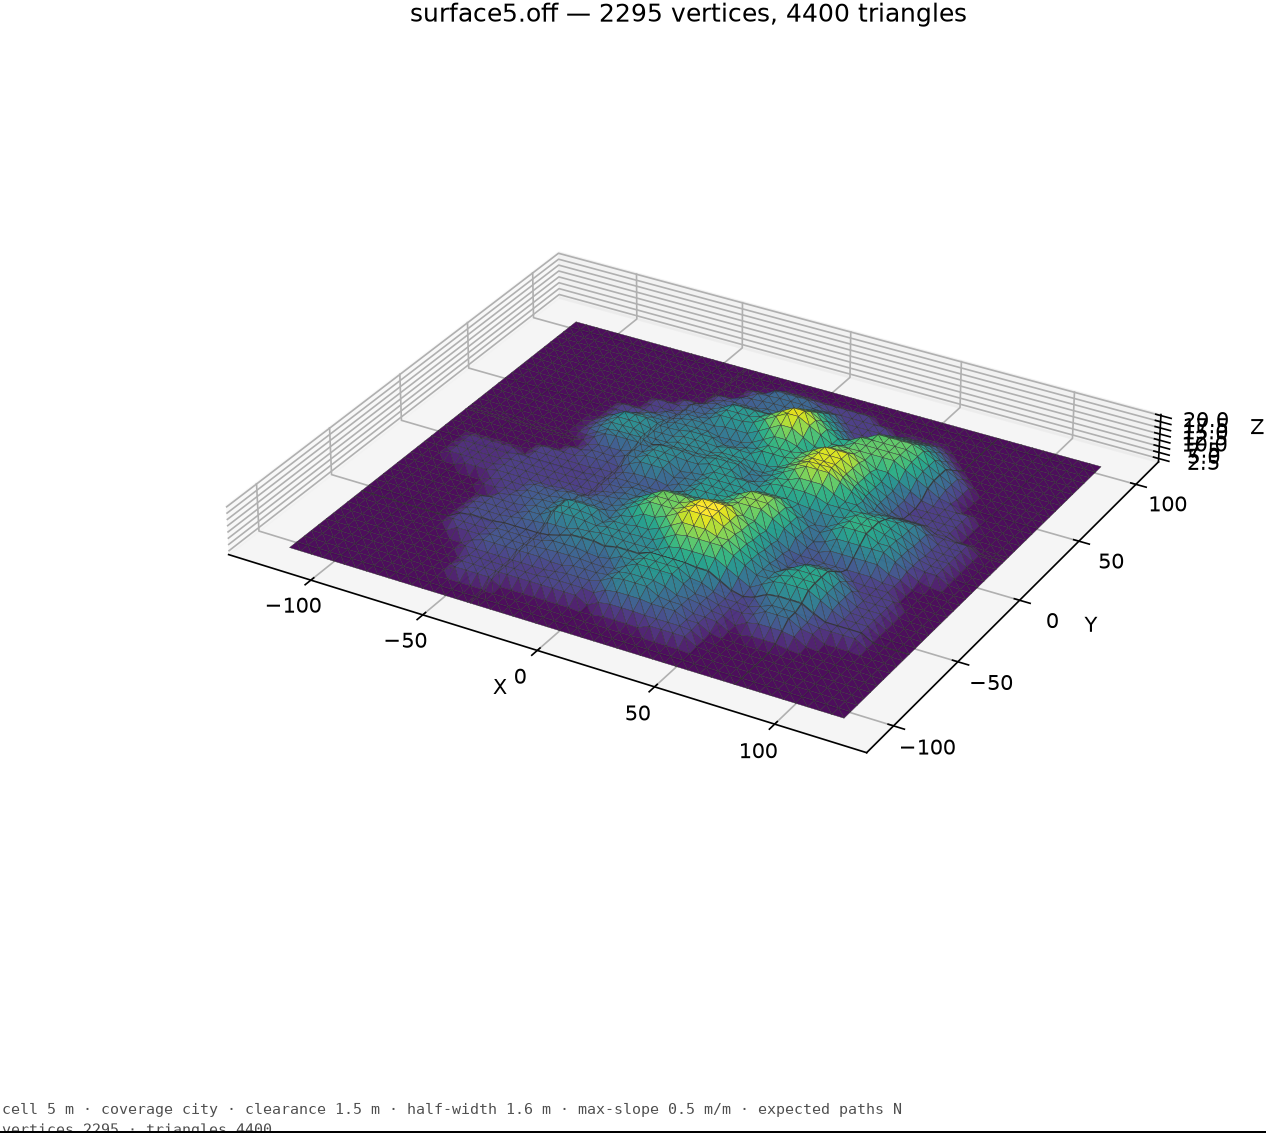
\includegraphics[width=\linewidth]{Figures/crop/repo_surface5.png}
    \caption{Lưới $5$ m: 2\,295 đỉnh, 4\,400 tam giác.}
  \end{subfigure}\par\vspace{2pt}
  \begin{subfigure}{0.60\textwidth}
    \centering
    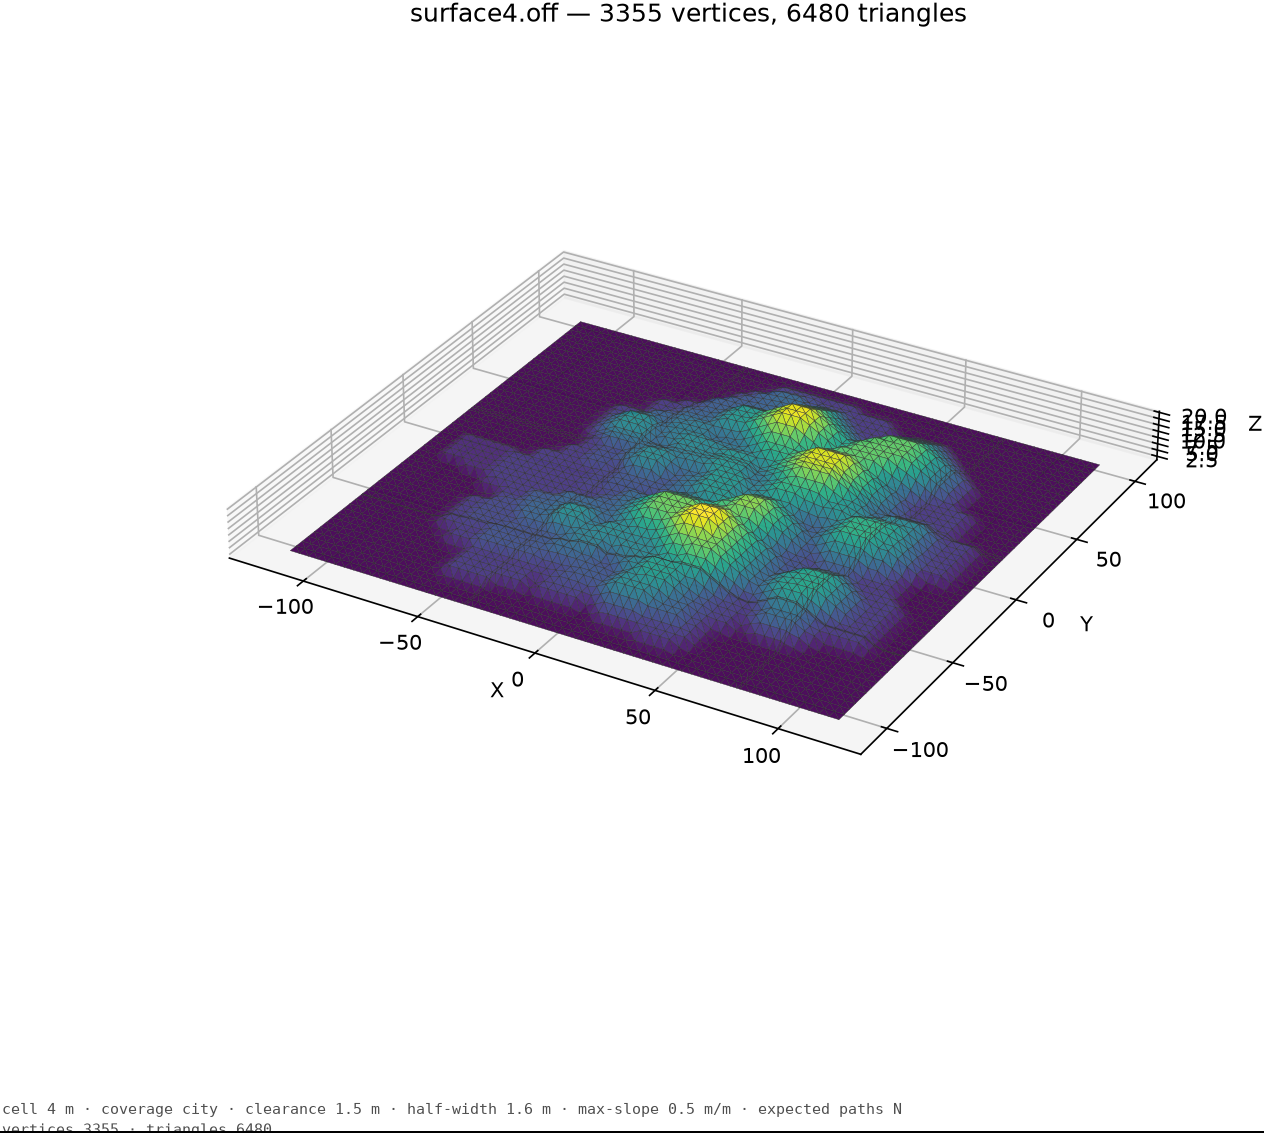
\includegraphics[width=\linewidth]{Figures/crop/repo_surface4.png}
    \caption{Lưới $4$ m: 3\,355 đỉnh, 6\,480 tam giác.}
  \end{subfigure}
  \caption{Hai bề mặt dẫn đường dựng từ cùng một scene, chỉ khác kích thước ô:
    lưới $5$ m (trên) và lưới $4$ m (dưới). Màu là cao độ; các gờ sáng là vùng có
    công trình cao bên dưới.}
  \label{fig:surfaces-54}
\end{figure*}

\begin{figure*}[!t]
  \centering
  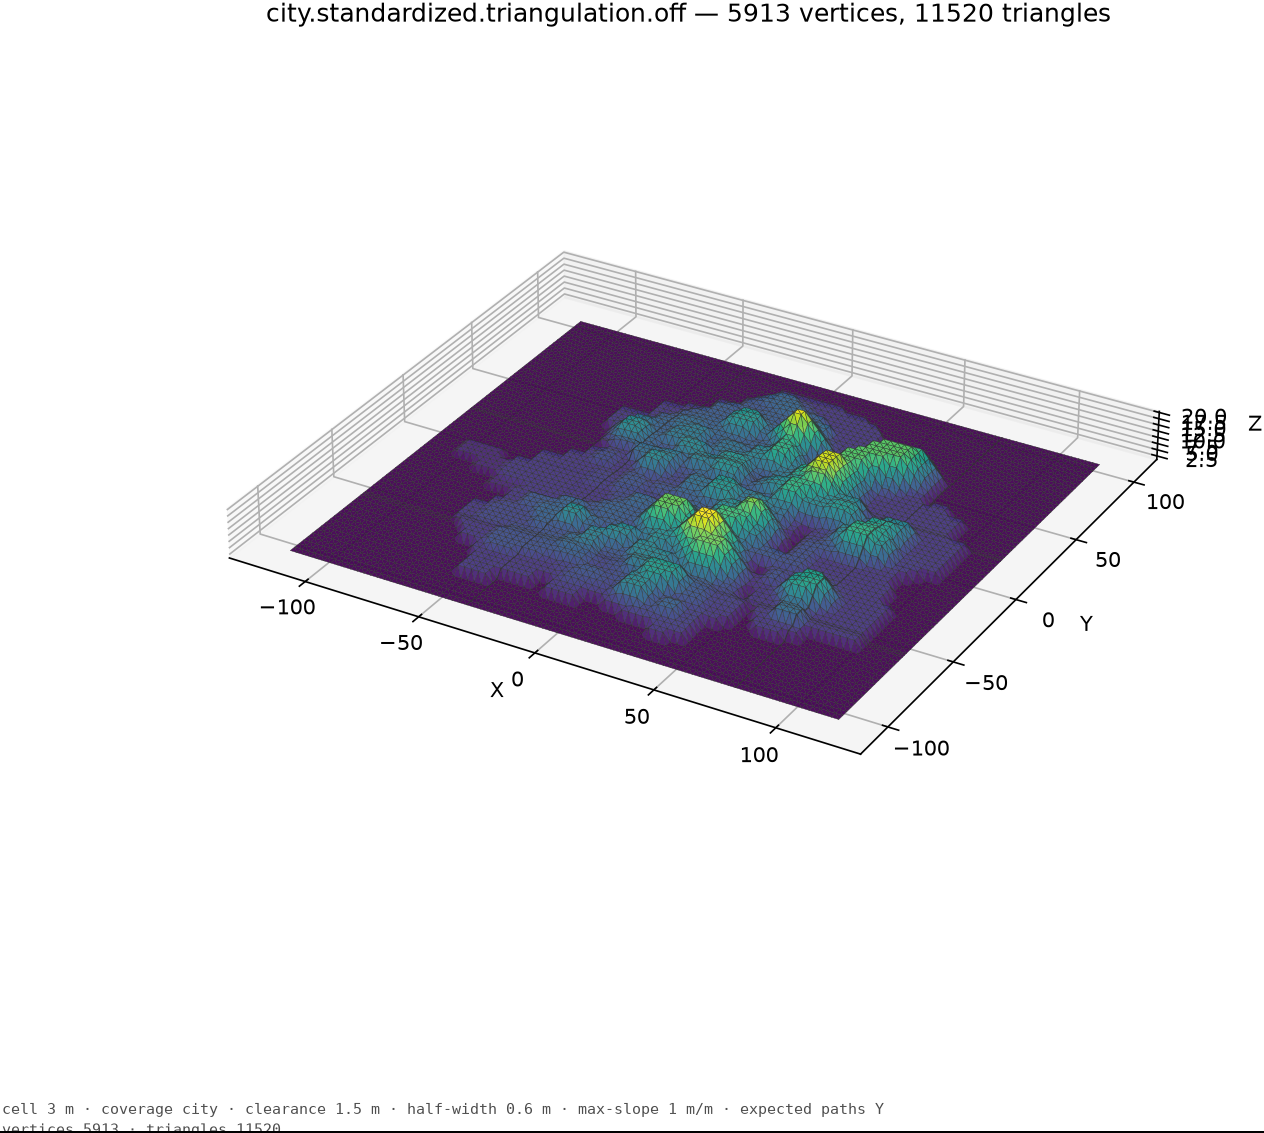
\includegraphics[width=0.75\textwidth]{Figures/crop/repo_surface3.png}
  \caption{Bề mặt dẫn đường lưới $3$ m: 5\,913 đỉnh, 11\,520 tam giác. So với hai
    lưới trên, mật độ tam giác cao hơn và các vách dốc $45^\circ$ rõ hơn.}
  \label{fig:surface-3}
\end{figure*}

Hình~\ref{fig:surfaces-54} và Hình~\ref{fig:surface-3} cho thấy mật độ tam giác
tăng rõ từ lưới $5$ lên lưới $4$ rồi lưới $3$, trong khi hình dạng tổng thể của
envelope vẫn giữ các “dãy” cao độ theo công trình. Lưới $5$ và $4$ dùng cùng dự
phòng ngang và cùng độ dốc, nên khác biệt chủ yếu là độ mịn; lưới $3$ có thêm các
vách dốc $45^\circ$ và bám sát hình học hơn, thể hiện ở các gờ nhọn và vùng
chuyển tiếp hẹp hơn. Đây là hình ảnh định tính tương ứng với các số đo ở
Bảng~\ref{tab:surfaces}.

\begin{figure*}[!t]
  \centering
  \begin{subfigure}{0.62\textwidth}
    \centering
    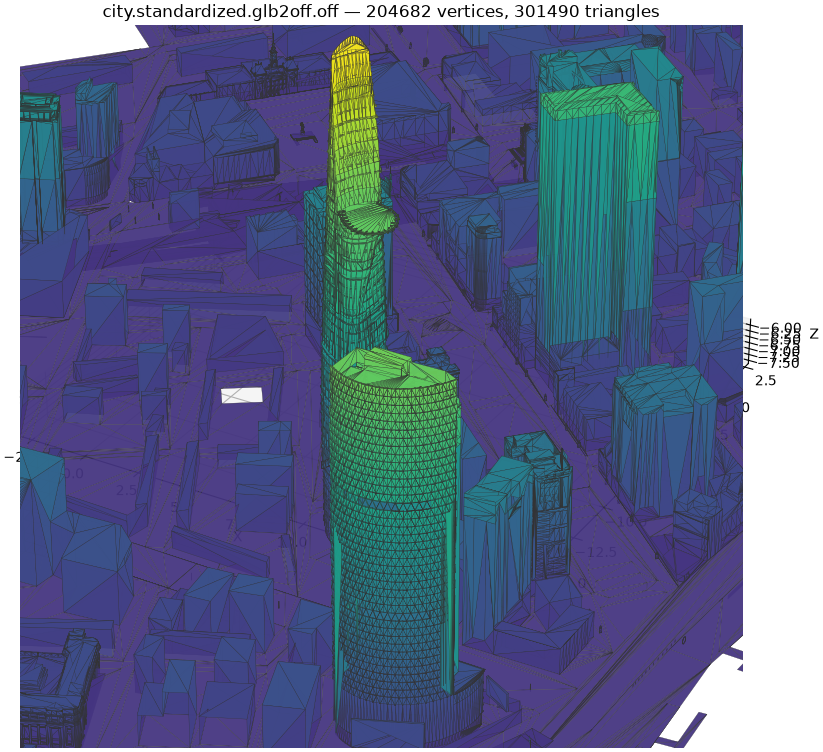
\includegraphics[width=\linewidth]{Figures/crop/etc_city_close.png}
    \caption{Cận cảnh scene: các khối nhà và tháp được tô theo độ cao.}
  \end{subfigure}\par\vspace{2pt}
  \begin{subfigure}{0.62\textwidth}
    \centering
    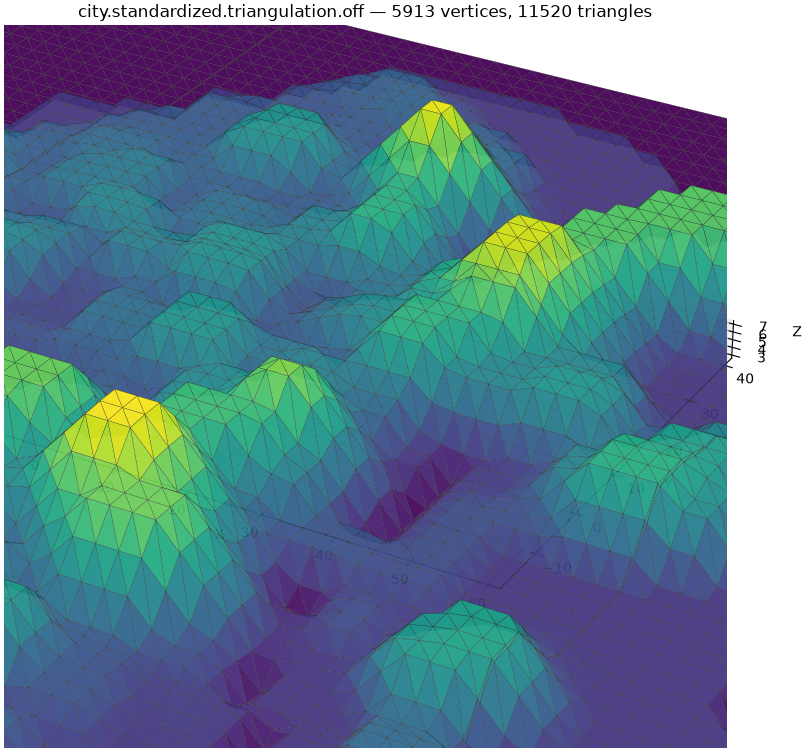
\includegraphics[width=\linewidth]{Figures/crop/etc_surface_close.png}
    \caption{Cận cảnh bề mặt: các tam giác phủ lên công trình và tạo đỉnh/dốc.}
  \end{subfigure}
  \caption{Cận cảnh scene thành phố và bề mặt dẫn đường. Bề mặt không sao chép
    mái nhà; nó nâng lên theo hộp bao công trình rồi hạ dần thành ramp, nên các
    đỉnh tam giác nằm phía trên nóc nhà.}
  \label{fig:city-data}
\end{figure*}

Hình~\ref{fig:city-data} cho thấy rõ hơn quan hệ giữa hai lớp: panel (a) là hình
học công trình với các tháp cao thấp khác nhau; panel (b) là cùng vùng đó nhưng
đã được phủ bởi lưới tam giác của envelope. Các tam giác có kích thước đều theo
ô, nhưng cao độ thay đổi theo công trình bên dưới, tạo ra các “đỉnh” và “yên
ngựa” mà tuyến phải đi qua. Đây là lý do đường đi trên bề mặt không trùng với
đường chim bay và có thể dài hơn khoảng cách Euclid.

\begin{figure*}[!t]
  \centering
  \begin{subfigure}{0.62\textwidth}
    \centering
    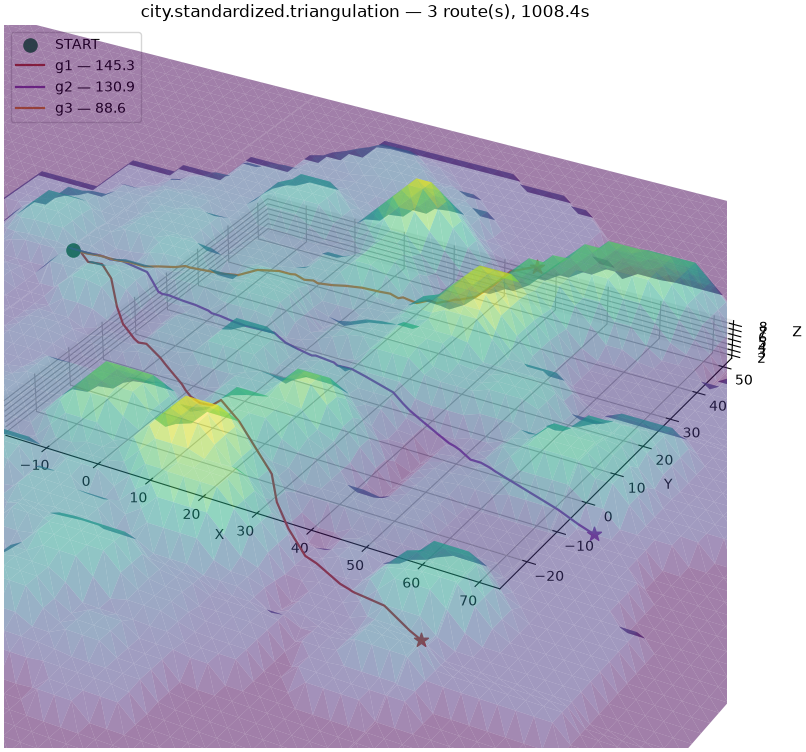
\includegraphics[width=\linewidth]{Figures/crop/etc_routes_3d.png}
    \caption{Góc nhìn 3D: tuyến bám theo các đỉnh và dốc của envelope.}
  \end{subfigure}\par\vspace{2pt}
  \begin{subfigure}{0.62\textwidth}
    \centering
    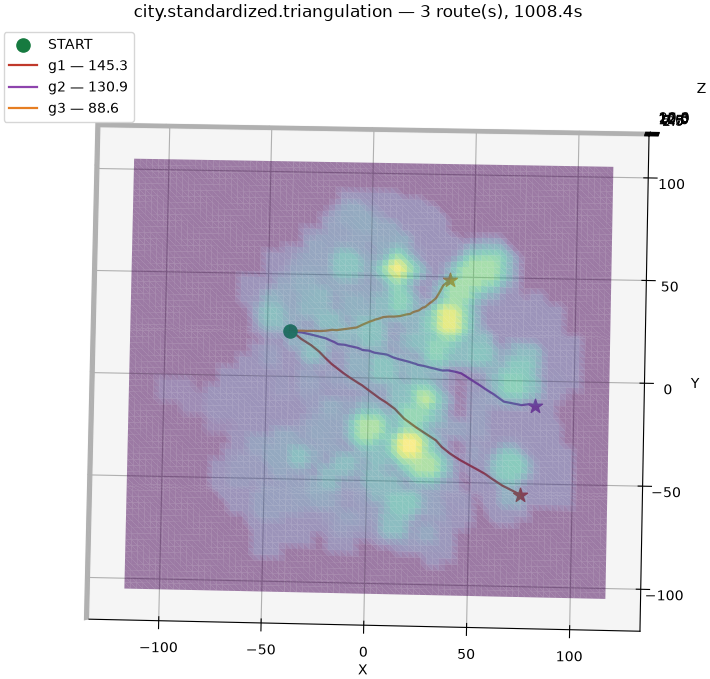
\includegraphics[width=\linewidth]{Figures/crop/etc_routes_top.png}
    \caption{Hình chiếu bằng: ba tuyến từ cùng một nguồn đến ba đích.}
  \end{subfigure}
  \caption{Cận cảnh tuyến trên bề mặt lưới $3$ m. Panel (a) cho thấy độ cao thay
    đổi dọc tuyến; panel (b) cho thấy hình dạng ngang và việc các tuyến tách
    nhau ngay sau nguồn.}
  \label{fig:routes-detail}
\end{figure*}


\subsection{Lập tuyến và đối chiếu tham chiếu}\label{sec:stage-plan}

Funnel Tree chạy trên từng mission. Với mission nhiều goal, mỗi goal được tìm
trong một lượt riêng: một lượt chung giữ frontier theo goal xa nhất và làm số lần
lan truyền tăng mạnh trên bề mặt thành phố, nên chế độ \texttt{per-goal} được
chọn cho phần thành phố. Đánh đổi là ưu thế một nguồn -- mọi đích của thuật toán
không được khai thác trọn vẹn. Trên đồ thị nguồn phụ, thuật toán dùng A* với
heuristic Euclid $h(v)=\norm{v-g}$ (khi tắt heuristic, hàng đợi ưu tiên thoái hóa
thành Dijkstra); mỗi đỉnh được settle một lần rồi lan truyền phễu. Giới hạn thời gian áp cho từng lượt
tìm, giới hạn số nút chặn lan truyền bùng nổ, và Thủ tục 2 được bật.

Mỗi route ghi waypoint 3D, độ dài (tổng Euclid giữa các waypoint), số lần lan
truyền, thời gian từng goal, cùng hash của mission, mesh và mã thuật toán. Nhờ đó
một dòng trong bảng có thể truy ngược về đúng đầu vào sinh ra nó. Bảng~\ref{tab:planning}
trình bày độ dài, số waypoint và chi phí tìm kiếm của ba cấu hình. Độ dài là tổng
khoảng cách giữa các waypoint trên bề mặt, tính trước bước rút gọn Douglas--Peucker
với dung sai $0{,}1$ dùng cho chuyến bay; sau rút gọn, số waypoint mà plugin thực
sự bay là $27/25/24$ (lưới $5$), $27/24/26$ (lưới $4$) và $30/38/33$ (lưới $3$).

\begin{table*}[!t]
  \caption{Độ dài tuyến và chi phí lập tuyến trên ba bề mặt. $L$ tính bằng mét của
    mô hình thu nhỏ; $w$ là số waypoint trước khi rút gọn; $P$ là số lần lan truyền của
    từng goal; $T_{\rm plan}$ là thời gian tường của cả ba lượt tìm.}
  \label{tab:planning}
  {\fontsize{7}{8.6}\selectfont
  \begin{adjustbox}{max width=\textwidth}
  \begin{tabular}{@{}lrrrrrrrrr@{}}
    \toprule
    Cấu hình & $L_{\rm G1}$ & $L_{\rm G2}$ & $L_{\rm G3}$
      & $w_{\rm G1}/w_{\rm G2}/w_{\rm G3}$
      & $P_{\rm G1}$ & $P_{\rm G2}$ & $P_{\rm G3}$ & $\sum P$ & $T_{\rm plan}$ (s) \\
    \midrule
    lưới $5$ & 142,418722 & 125,636333 & 86,152328 & 41/46/40 & 49  & 34  & 21  & 104 & 44,984 \\
    lưới $4$ & 142,909050 & 127,295935 & 86,194146 & 50/59/48 & 81  & 66  & 40  & 187 & 186,175 \\
    lưới $3$ & 145,314559 & 130,891670 & 88,611502 & 65/73/68 & 177 & 150 & 102 & 429 & 1\,008,389 \\
    \bottomrule
  \end{tabular}
  \end{adjustbox}}
\end{table*}

Số lần lan truyền tăng từ $104$ lên $187$ rồi $429$ khi số tam giác tăng từ
$4\,400$ lên $6\,480$ rồi $11\,520$. Thời gian tường tăng nhanh hơn: từ
\num{44.984} giây lên \num{186.175} giây (gấp $4{,}1$ lần) và \num{1008.389}
giây (gấp $5{,}4$ lần so với lưới $4$). Mỗi cấu hình chỉ được đo một lượt trên
máy chưa khống chế tải, nên các tỉ lệ này chỉ là số liệu quan sát, không dùng để
suy ra độ phức tạp tiệm cận.

Độ dài tuyến tăng khi lưới mịn hơn, nhưng mức tăng không đều: G1 từ
\num{142.418722} lên \num{142.909050} rồi \num{145.314559}; G2 từ
\num{125.636333} lên \num{127.295935} rồi \num{130.891670}. Một phần chênh lệch
đến từ bề mặt mịn hơn bám sát khối công trình hơn và tạo nhiều chỗ lượn hơn,
phần khác đến từ điểm đích được snap lại như đã nêu.

Năm mesh nhỏ có đường tham chiếu độc lập; bước đối chiếu chạy Funnel từ đúng đỉnh
nguồn ghi trong tham chiếu, so độ dài từng polyline với dung sai tương đối
$10^{-4}$; không có đỉnh nào vượt dung sai trên tổng 76 đỉnh. Bốn mesh còn lại và bề mặt
thành phố không có tham chiếu độc lập, nên không có bộ giải thứ hai để khẳng định
tối ưu.

Thay vào đó, tuyến thành phố được kiểm tra bằng một cặp cận độc lập trên chính bề
mặt lưới $3$ m (tệp bề mặt có tám ký tự đầu SHA256 là \texttt{9cec5d09}, trùng
dòng lưới $3$ trong Bảng~\ref{tab:surfaces}). Cận dưới là khoảng cách Euclid $d_E=\norm{x_g-x_s}$, vì mọi đường
trên bề mặt không ngắn hơn đoạn thẳng trong không gian. Cận trên $\ell_G$ là độ
dài đường đi ngắn nhất trên đồ thị cạnh của lưới (Dijkstra theo trọng số là độ dài
cạnh); đường này nằm trọn trên bề mặt nên không thể ngắn hơn đường trắc địa. Mọi
độ dài Funnel Tree phải nằm trong khoảng $[d_E,\ell_G]$, và Bảng~\ref{tab:bounds}
cho thấy cả ba tuyến đều thỏa. Đây là điều kiện cần, không phải chứng minh tối ưu:
khoảng cách tới cận trên còn $4{,}6\,\%$, $4{,}9\,\%$ và $22{,}3\,\%$, phản ánh
việc đường trên đồ thị cạnh bị buộc đi qua đỉnh nên vòng xa hơn, đặc biệt ở G3.

\begin{table}[!t]
  \caption{Kiểm tra kẹp độ dài tuyến trên lưới $3$ m. $d_E$ là cận dưới Euclid,
    $L$ là độ dài Funnel Tree, $\ell_G$ là cận trên từ Dijkstra trên đồ thị cạnh;
    đơn vị là mét của mô hình thu nhỏ.}
  \label{tab:bounds}
  {\fontsize{6.5}{8}\selectfont
  \setlength{\tabcolsep}{3pt}%
  \begin{tabular}{@{}lrrrr@{}}
    \toprule
    Goal & $d_E$ & $L$ & $\ell_G$ & $(\ell_G{-}L)/L$ \\
    \midrule
    g1 & 137,409 & 145,314559 & 151,981 & 4,59\,\% \\
    g2 & 124,533 & 130,891670 & 137,266 & 4,87\,\% \\
    g3 &  82,138 &  88,611502 & 108,404 & 22,34\,\% \\
    \bottomrule
  \end{tabular}}
\end{table}

Cặp cận này chỉ chạy được cho lưới $3$ m vì đây là bề mặt được công bố kèm dữ
liệu; hai lưới còn lại chỉ có route và manifest, không có tệp bề mặt đầy đủ trong
bộ kết quả lưu trữ. Hình~\ref{fig:routes-small} minh họa đầu ra của công cụ vẽ tuyến trên
bảy mesh còn lại; cùng với \texttt{icosahedron} và \texttt{J17}, cả chín mesh đều
có ảnh tuyến.

\begin{figure*}[!t]
  \centering
  \begin{subfigure}{0.235\textwidth}
    \centering
    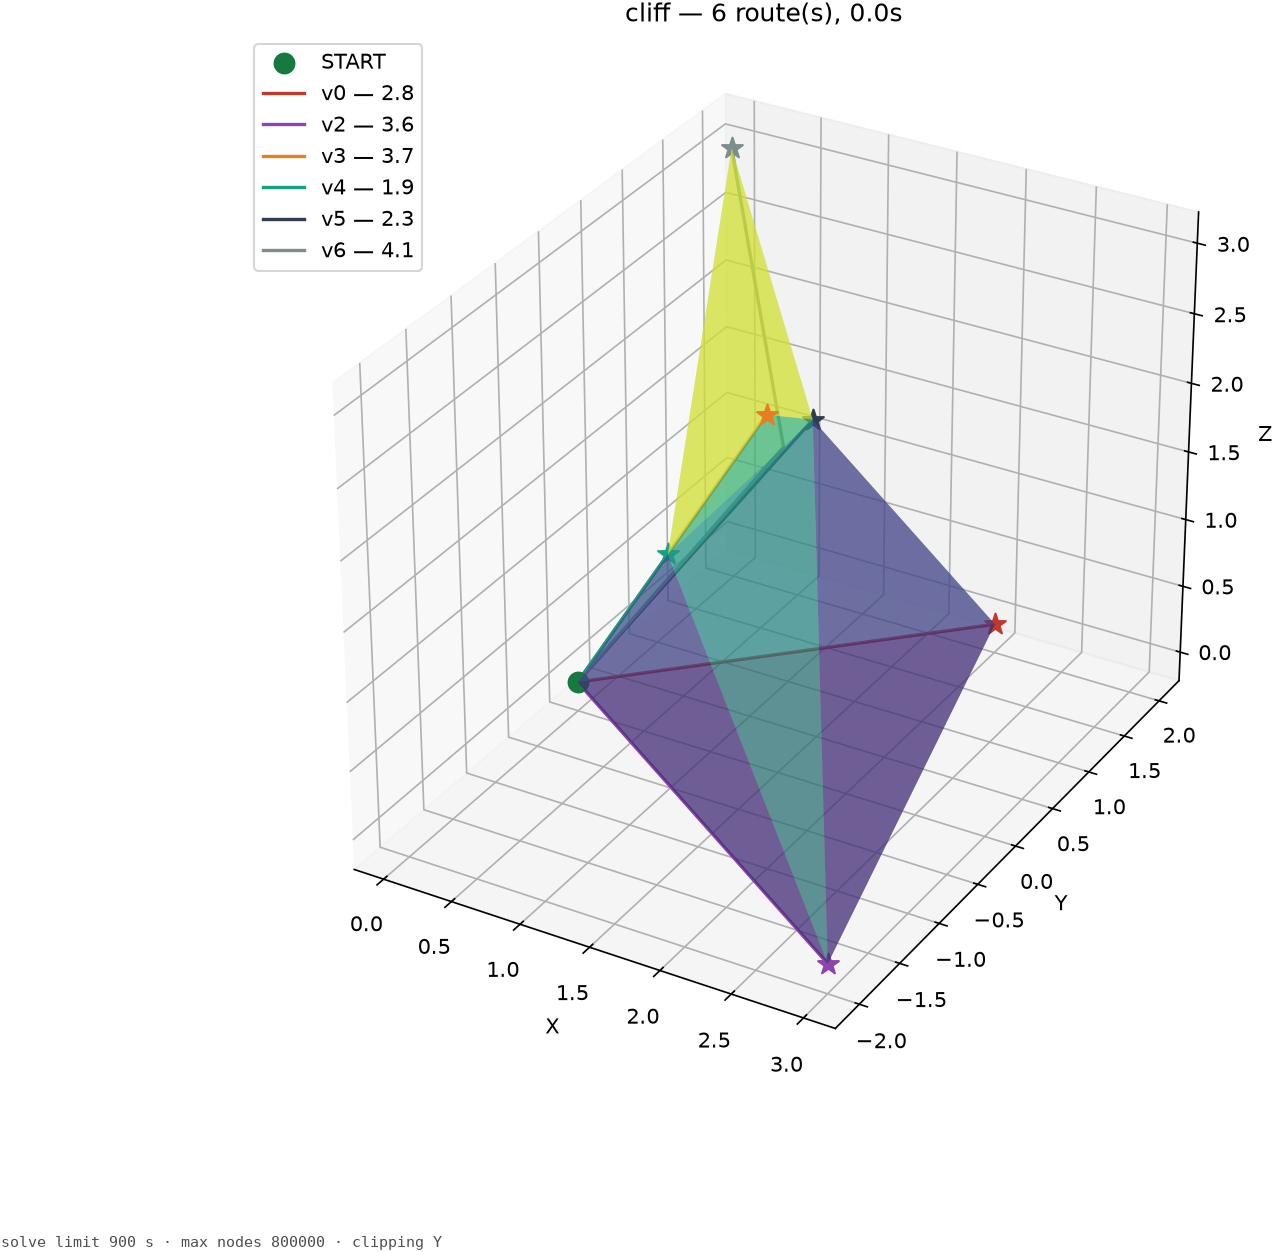
\includegraphics[width=\linewidth]{Figures/crop/repo_cliff_routes.png}
    \caption{\texttt{cliff}}
  \end{subfigure}\hfill
  \begin{subfigure}{0.235\textwidth}
    \centering
    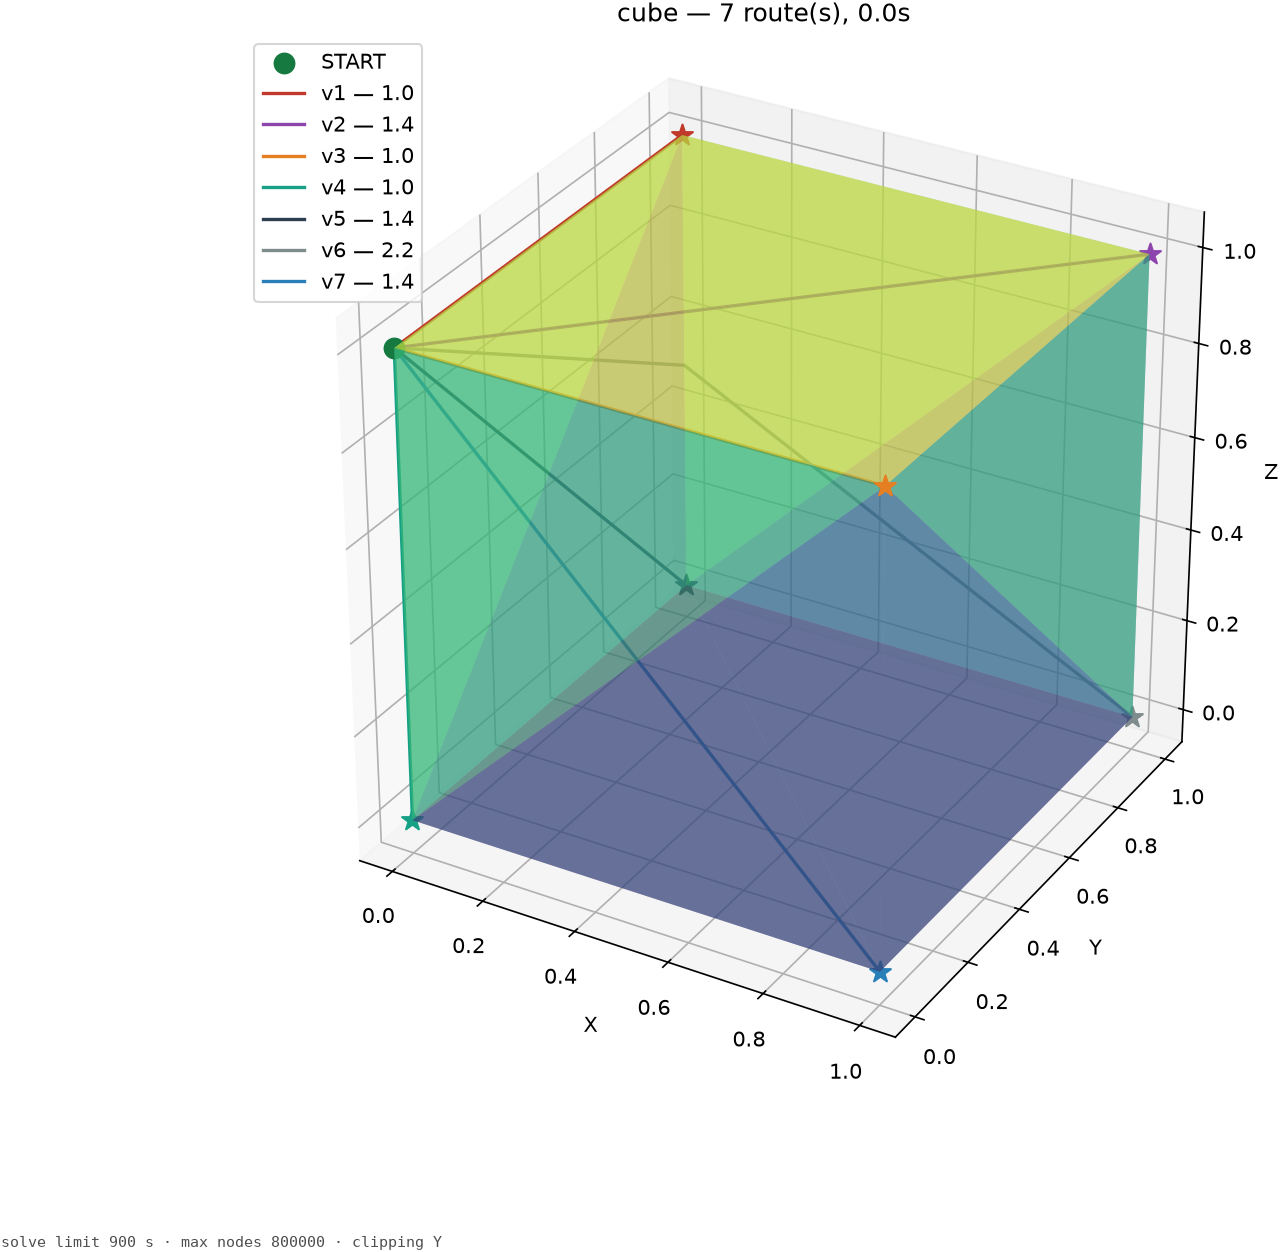
\includegraphics[width=\linewidth]{Figures/crop/repo_cube_routes.png}
    \caption{\texttt{cube}}
  \end{subfigure}\hfill
  \begin{subfigure}{0.235\textwidth}
    \centering
    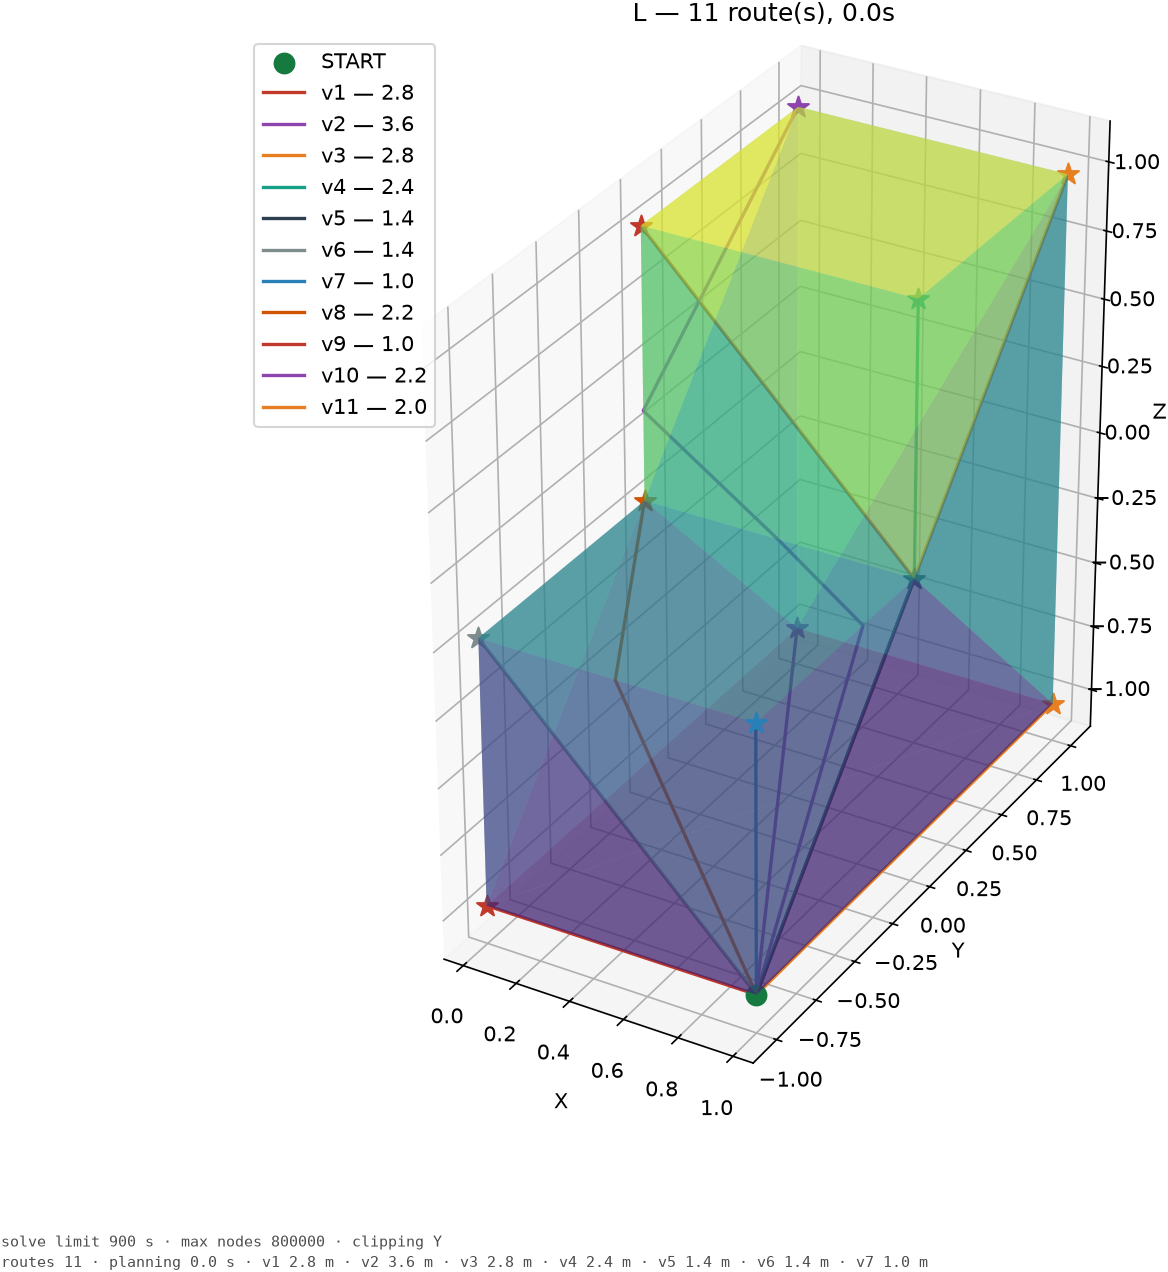
\includegraphics[width=\linewidth]{Figures/crop/repo_L_routes.png}
    \caption{\texttt{L}}
  \end{subfigure}\hfill
  \begin{subfigure}{0.235\textwidth}
    \centering
    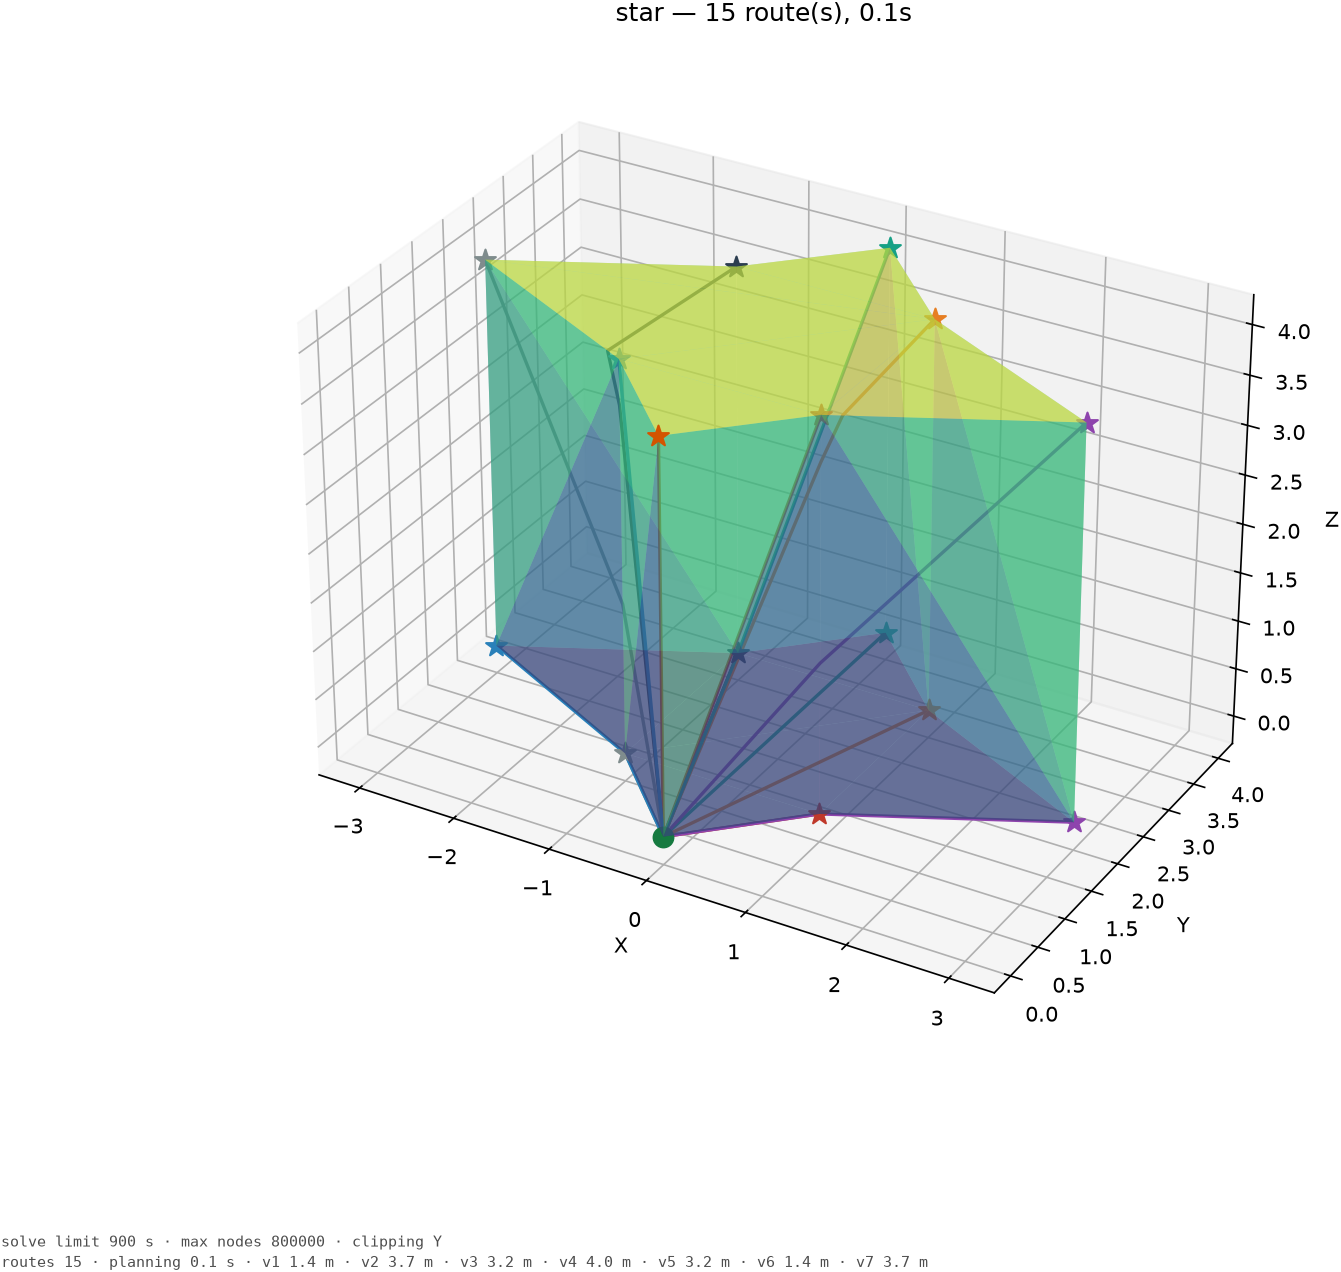
\includegraphics[width=\linewidth]{Figures/crop/repo_star_routes.png}
    \caption{\texttt{star}}
  \end{subfigure}\par\vspace{2pt}
  \hspace*{\fill}%
  \begin{subfigure}{0.235\textwidth}
    \centering
    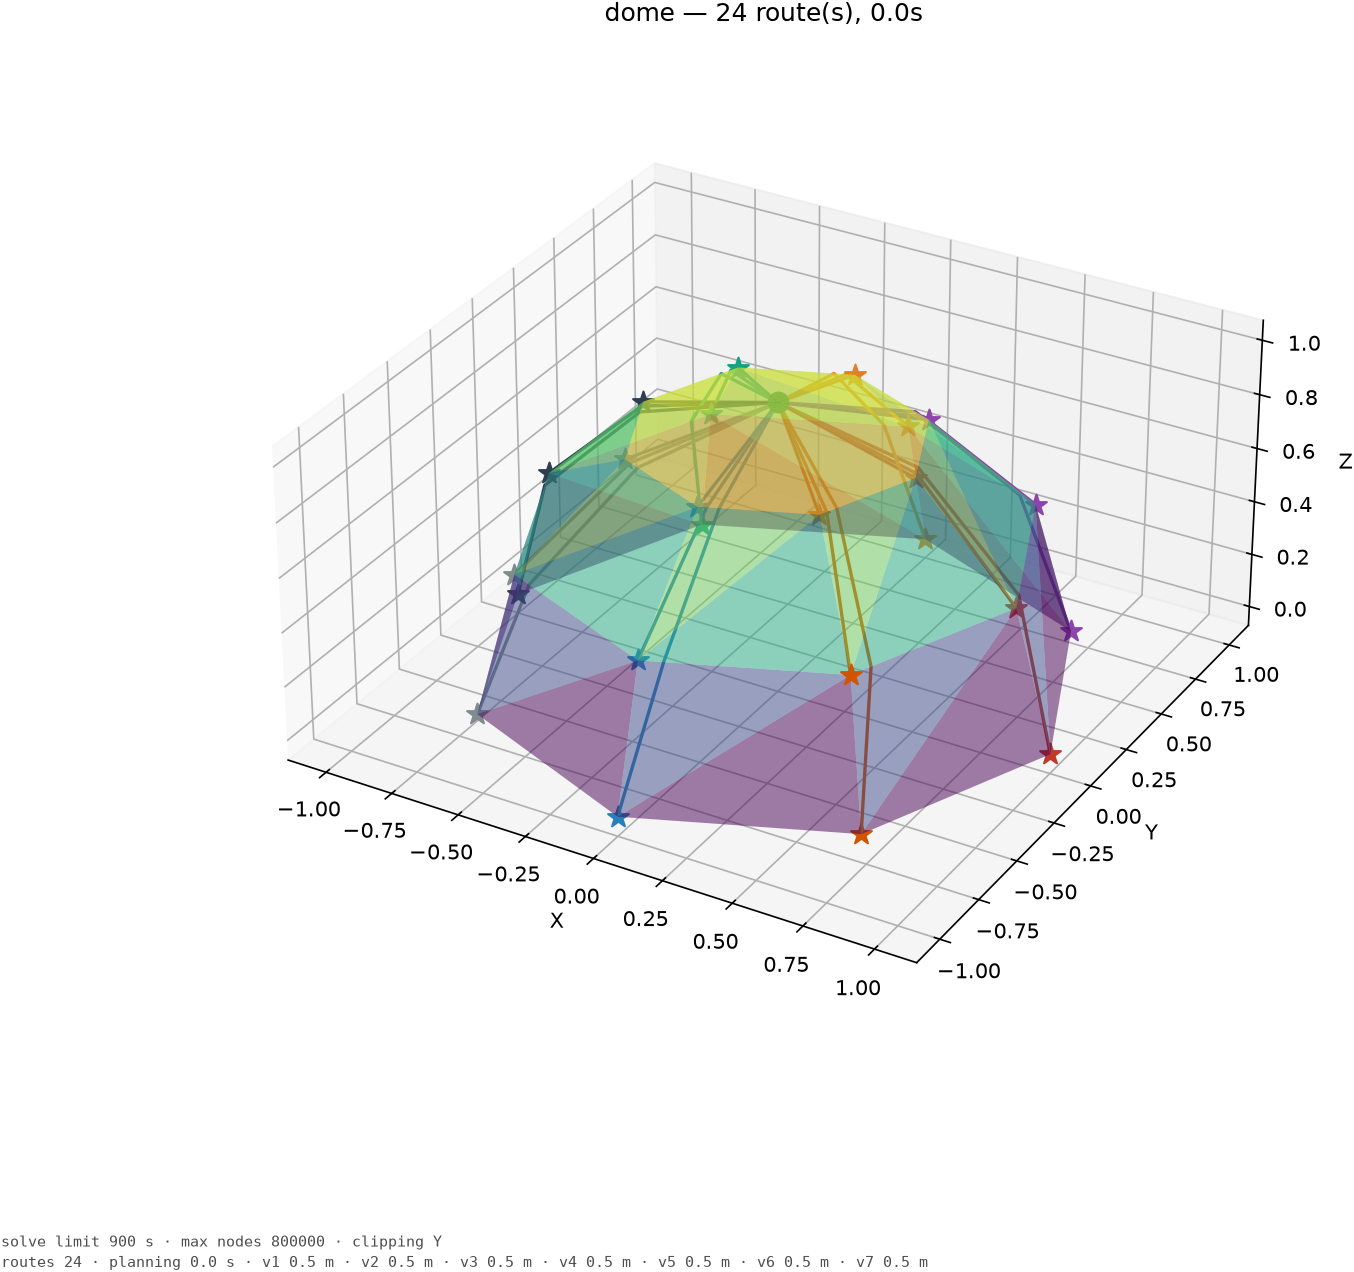
\includegraphics[width=\linewidth]{Figures/crop/repo_dome_routes.png}
    \caption{\texttt{dome}}
  \end{subfigure}\hfill
  \begin{subfigure}{0.235\textwidth}
    \centering
    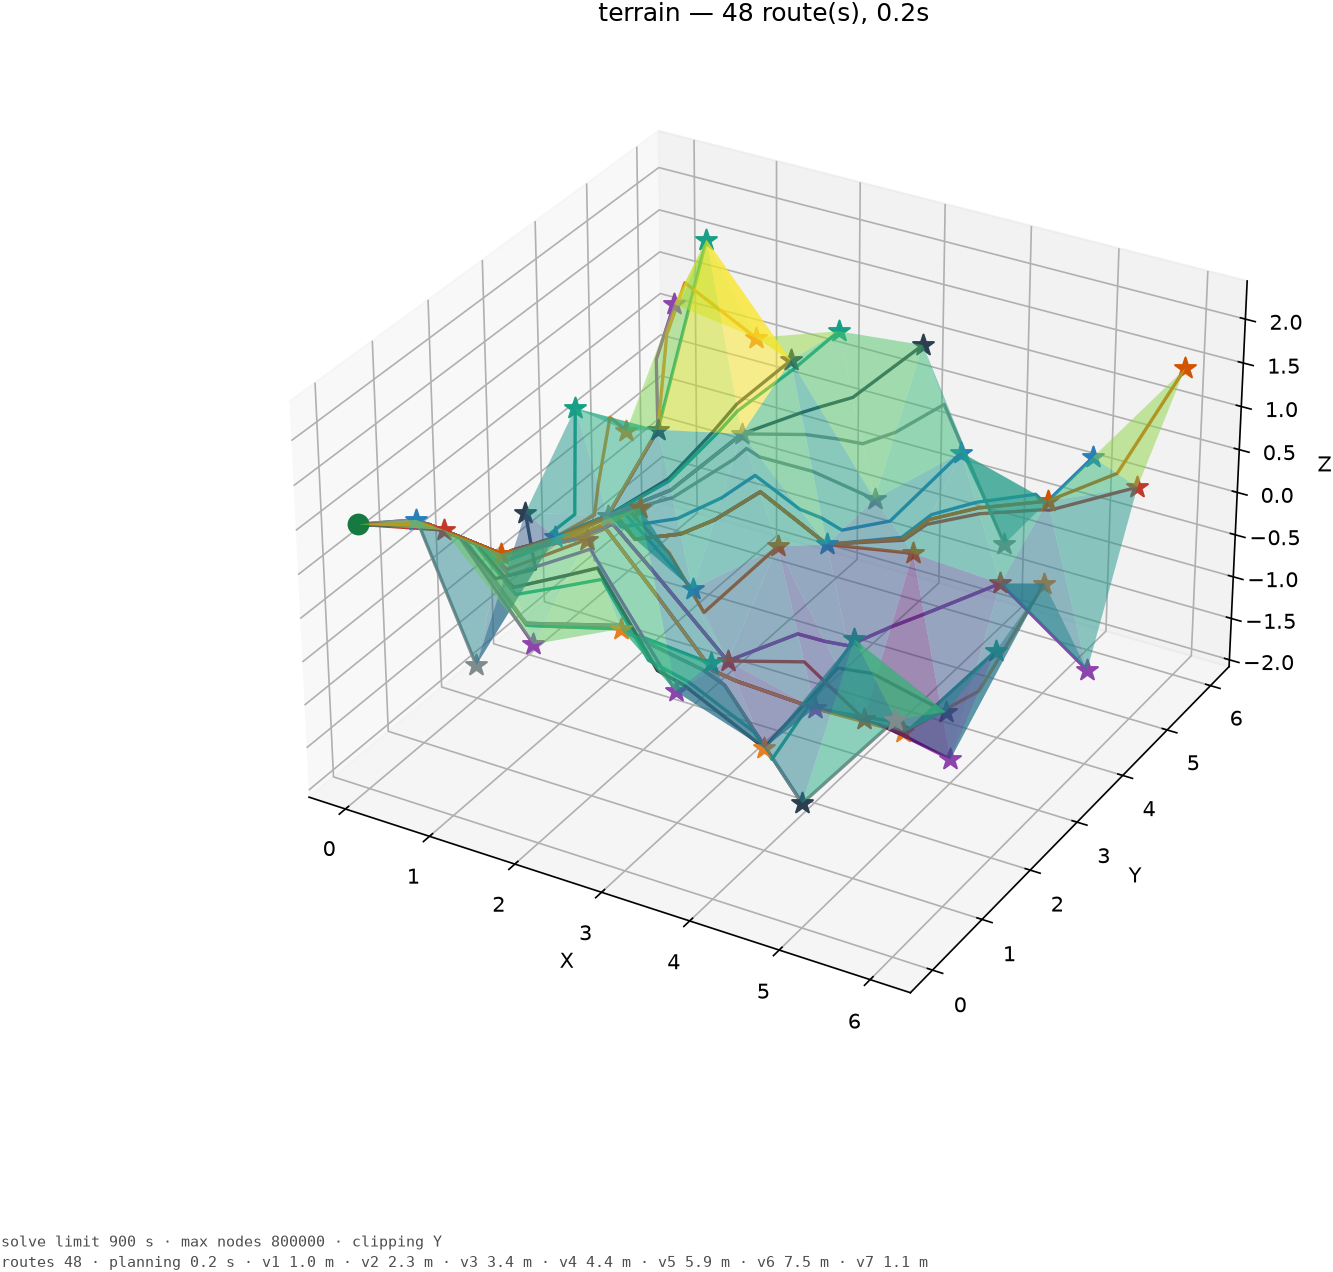
\includegraphics[width=\linewidth]{Figures/crop/repo_terrain_routes.png}
    \caption{\texttt{terrain}}
  \end{subfigure}\hfill
  \begin{subfigure}{0.235\textwidth}
    \centering
    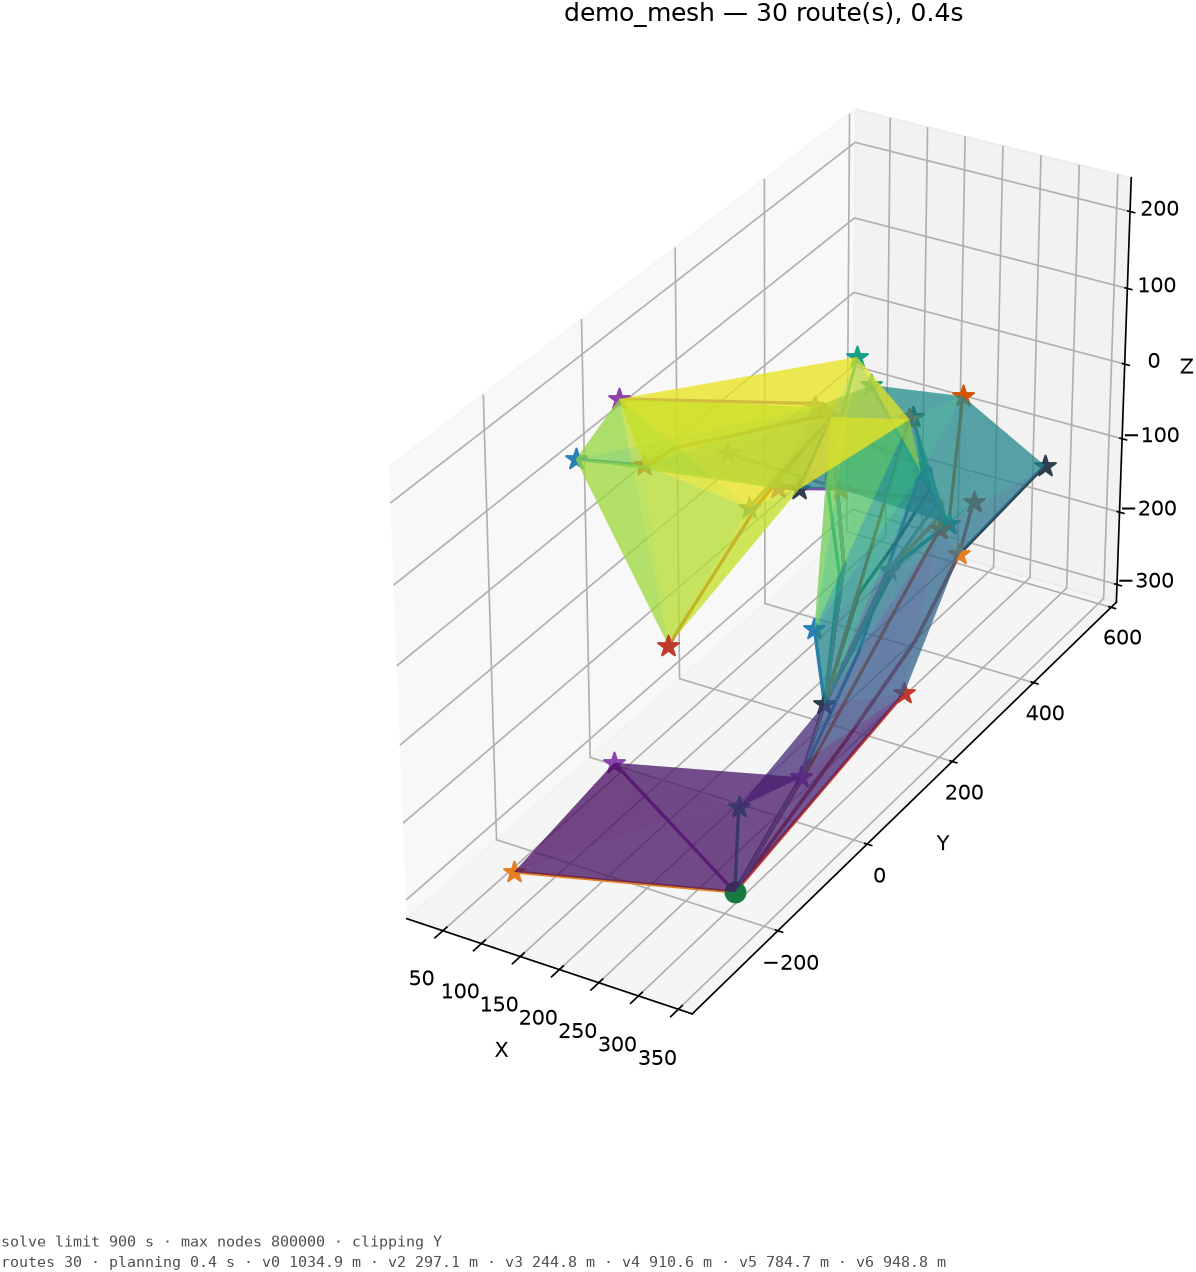
\includegraphics[width=\linewidth]{Figures/crop/repo_demo_mesh_routes.png}
    \caption{\texttt{demo\_mesh}}
  \end{subfigure}%
  \hspace*{\fill}
  \caption{Đầu ra của công cụ vẽ tuyến trên bảy mesh còn lại. Cùng với
    \texttt{icosahedron} và \texttt{J17}, cả chín mesh của bộ dữ liệu đều có ảnh
    tuyến.}
  \label{fig:routes-small}
\end{figure*}

Hình~\ref{fig:routes-small} cho thấy công cụ vẽ tuyến giữ được hình dạng đặc
trưng của từng mesh: \texttt{cliff} có các tuyến gãy qua sườn dốc, \texttt{star}
có các nhánh tỏa theo múi, \texttt{dome} và \texttt{terrain} có tuyến men theo
biên mở, còn \texttt{demo\_mesh} có tuyến vòng qua lỗ xuyến. Đây là kiểm tra định
tính rằng cùng một quy trình lập tuyến chạy được trên bề mặt kín, không lồi và mở;
phần định lượng vẫn là đối chiếu độ dài ở Bảng~\ref{tab:ket-qua-tong-the}.

\subsection{Mô hình UAV, quỹ đạo và telemetry}\label{sec:trajectory}

Đường hình học do Funnel Tree trả về là một polyline trên bề mặt. Để tránh dừng
lại ở mỗi waypoint, quỹ đạo tham chiếu được dựng bằng spline Catmull--Rom đi qua
toàn bộ waypoint. Với các điểm $p_0,\ldots,p_{n-1}$, tiếp tuyến tại $p_i$ là
\begin{equation}
  m_i=
  \begin{cases}
    p_1-p_0, & i=0,\\
    \tfrac12\left(p_{i+1}-p_{i-1}\right), & 0<i<n-1,\\
    p_{n-1}-p_{n-2}, & i=n-1,
  \end{cases}
  \label{eq:tangent}
\end{equation}
và vị trí trên đoạn $p_i\to p_{i+1}$ là
\begin{equation}
  \begin{split}
    q(u)={}&h_{00}(u)\,p_i+h_{10}(u)\,m_i\\
         &+h_{01}(u)\,p_{i+1}+h_{11}(u)\,m_{i+1},
  \end{split}
  \label{eq:catmullrom}
\end{equation}
với $0\le u\le 1$, trong đó $h_{00}=2u^3-3u^2+1$,
$h_{10}=u^3-2u^2+u$, $h_{01}=-2u^3+3u^2$ và $h_{11}=u^3-u^2$. Chính cơ sở
Hermite bảo đảm $q(0)=p_i$ và $q(1)=p_{i+1}$ với mọi cách chọn tiếp tuyến;
\eqref{eq:tangent} chỉ quyết định hình dạng đoạn cong giữa hai đầu. Spline được
lấy mẫu cách khoảng $0{,}2$ đơn vị để tính chiều dài cung; vận tốc và hướng tiếp
tuyến liên tục, và phương tiện chỉ dừng ở điểm cuối.

Trên toàn tuyến, một profile vận tốc thang duy nhất gồm ba pha tăng tốc, chạy đều
và giảm tốc được dùng, với tốc độ lớn nhất $v_{\max}=5$ và gia tốc
$a_{\max}=3$. Nếu chiều dài cung $L$ đủ lớn, thời gian tăng tốc là
$T_r=v_{\max}/a_{\max}$ và quãng đường tăng tốc là
$d_r=v_{\max}^2/(2a_{\max})$; ngược lại profile có dạng tam giác với
$v_{\rm peak}=\sqrt{a_{\max}L}$ và $T=2\sqrt{L/a_{\max}}$. Nhiệm vụ có thời gian
chờ khởi đầu $2$ giây và không có thời gian giữ tại waypoint.

Bộ điều khiển dùng vị trí và vận tốc đo trực tiếp từ trạng thái mô phỏng, với
gia tốc lệnh
\begin{equation}
  a_{\mathrm{cmd}}=a_{\mathrm{ff}}+K_p(q-x)+K_d(\dot q-\dot x),
  \label{eq:control}
\end{equation}
trong đó $a_{\mathrm{ff}}$ là gia tốc bù trước của quỹ đạo, gồm thành phần tiếp
tuyến của profile và thành phần hướng tâm $v^2\,\mathrm{d}T/\mathrm{d}s$ được chặn
trong $[-3,3]$ theo từng trục; $K_p=2{,}5$ và $K_d=3{,}2$; mỗi thành phần của
$a_{\mathrm{cmd}}$ được chặn trong $[-6,6]$. Lực tác dụng tại tâm khối lượng được
tính từ gia tốc lệnh và phần bù trọng lực.

UAV là một vật thể $1$ kg có va chạm thân hộp; cánh quạt chỉ để hiển thị. Mô hình
chưa có điều khiển tư thế, động lực học rotor, cảm biến nhiễu, ước lượng trạng thái
hay autopilot, nên kết quả được diễn giải là kiểm tra bám tuyến của mô hình chịu
lực, không phải xác nhận khả năng bay thực. Telemetry ghi mỗi $0{,}1$ giây trong
khi vật lý chạy $1$ ms; sai số bám tại mẫu $k$ là $e_k=\norm{x_k-q_k}$. Bài báo
cáo sai số lớn nhất $e_{\max}=\max_k e_k$, sai số trung bình $\bar e$ trên toàn bộ
mẫu và sai số cuối $e_{\rm final}$ tại thời điểm kết thúc.

\subsection{Dựng world và chạy Gazebo}\label{sec:stage-simulate}

Mỗi goal có một world riêng. World dùng bản visual của thành phố có normal để
Gazebo tô sáng, một bản collision đã decimate bằng vertex clustering với ô
$1{,}0$, và một SDF đặt bước vật lý $0{,}001$ giây, trọng trường $9{,}8$, vật thể
$1$ kg cùng plugin điều khiển. Scene gốc có \num{301490} tam giác; tám tam giác
diện tích bằng không (sliver) bị loại khi ghi STL nên bản dùng để dựng world còn
\num{301482} tam giác. Từ bản này, collision giảm do decimate xuống \num{26296}
tam giác và từ \num{204682} xuống \num{12402} đỉnh, đủ giữ hình dạng để kiểm tra
độ cao nhưng nhẹ hơn cho vật lý. Tuyến kế hoạch
được vẽ bằng các ống trụ và chấm màu tại waypoint; camera đặt ở phía tây-nam để
khung trọn tuyến.

Trước khi bay, tuyến được rút gọn bằng Douglas--Peucker với dung sai $0{,}1$ và
ghi thành một tệp route riêng cho plugin. Với lưới $4$, G1 đi từ $50$ xuống $27$
waypoint; với lưới $3$, G1 đi từ $65$ xuống $30$. Plugin đọc route này, chạy
Catmull--Rom và profile vận tốc, rồi ghi telemetry cùng metadata của phiên.

Gazebo Jetty 10.5 \cite{gazebo} chạy với engine DART. Chế độ mặc định là container
từ image \texttt{ghcr.io/openrobotics/gazebo:jetty-full} (khoảng 3 GB), ghim bằng
digest; chế độ \texttt{--native} dùng Gazebo cài trên máy. Chạy headless thì không
mở GUI và tự dừng khi telemetry có \texttt{phase=complete}; chạy GUI cần X11 và
một backend render. Vật lý chạy trên CPU nên số đo bám tuyến không phụ thuộc GPU.
Bảng~\ref{tab:environment} ghi cấu hình máy và phiên bản dùng khi đo.

\begin{table*}[!t]
  \caption{Môi trường chạy của quy trình. Phiên bản trong image là phiên bản dùng
    khi bay; host dùng để chạy các bước dữ liệu và lập tuyến nếu không dùng
    container.}
  \label{tab:environment}
  {\fontsize{7}{8.6}\selectfont
  \begin{adjustbox}{max width=\textwidth}
  \begin{tabular}{@{}lp{300pt}@{}}
    \toprule
    Thành phần & Giá trị \\
    \midrule
    Host & NixOS 26.11; Intel Core i7-9850H (6 nhân/12 luồng); 15 GiB RAM;
      NVIDIA GeForce MX150; Docker 29.9.1 \\
    Python & 3.14.8 trên host; 3.12.3 trong image \\
    Thư viện & NumPy 2.5.4; Shapely 2.2.0; Matplotlib 3.11.2; Pillow 13.0.0 \\
    Gazebo & Jetty 10.5.0, engine DART, bước vật lý $1$ ms, hệ Z-up \\
    Image nền & \texttt{ghcr.io/openrobotics/gazebo@sha256:452ff649...08c7},
      khoảng 3 GB \\
    Image dự án & \texttt{uav-funnel-tree:pipeline}, dựng từ \texttt{Dockerfile} \\
    Compose & \texttt{pipeline} (NVIDIA qua CDI), \texttt{pipeline-intel}
      (/dev/dri), \texttt{pipeline-software} (llvmpipe) \\
    Runtime & \texttt{FUNNEL\_RUNTIME=native}, \texttt{FUNNEL\_PYTHON=/usr/bin/python3},
      có GUI hoặc headless \\
    \bottomrule
  \end{tabular}
  \end{adjustbox}}
\end{table*}

\subsection{Kết quả bám tuyến}\label{sec:stage-validate}

Một chuyến bay \emph{hợp lệ} nếu pha cuối là \texttt{complete} và
$e_{\rm final}\le\num{0.5}$; chuyến bay \emph{đạt mốc chất lượng} nếu ngoài ra
$e_{\max}\le\num{1.0}$. Hai tiêu chí tách riêng để một góc cua trễ không làm dừng
quy trình, nhưng vẫn được ghi nhận là trượt mốc. Đây là các ngưỡng kỹ thuật đặt
trước cho mô hình thu nhỏ, không suy ra từ dự phòng ngang $r$ hay khoảng hở đứng
$\delta$, và không phải bảo đảm an toàn va chạm.

Chín chuyến bay (ba cấu hình $\times$ ba đích) đều hợp lệ. Bảy chuyến đạt mốc;
hai chuyến trượt mốc đều ở G2, một ở lưới $5$ và một ở lưới $3$. Riêng lưới $4$
đạt mốc ở cả ba đích, với sai số lớn nhất $0{,}399$; $0{,}591$ và $0{,}601$.
Bảng~\ref{tab:tracking} tập hợp các chỉ số từ telemetry đã lưu.

\begin{table*}[!t]
  \caption{Kết quả bám tuyến của chín chuyến bay. $T$ là thời gian mô phỏng,
    $e_{\max}$ và $\bar e$ là sai số lớn nhất và trung bình, $e_{\rm final}$ là
    sai số cuối, $v_{\max}$ là vận tốc đo lớn nhất. Đơn vị là mét của mô hình thu
    nhỏ.}
  \label{tab:tracking}
  {\fontsize{7}{8.6}\selectfont
  \begin{adjustbox}{max width=\textwidth}
  \begin{tabular}{@{}llrrrrrrl@{}}
    \toprule
    Cấu hình & Goal & $T$ (s) & $e_{\max}$ & $\bar e$ & $e_{\rm final}$
      & $v_{\max}$ & Hợp lệ & Đạt mốc \\
    \midrule
    lưới $5$ & g1 & 35,859 & 0,3650 & 0,0666 & 0,0004 & 5,1027 & Có & Đạt \\
             & g2 & 33,143 & 1,0224 & 0,1105 & 0,0000 & 5,0411 & Có & Trượt \\
             & g3 & 24,997 & 0,8517 & 0,0893 & 0,0006 & 5,1533 & Có & Đạt \\
    \midrule
    lưới $4$ & g1 & 35,865 & 0,3994 & 0,0589 & 0,0000 & 5,1272 & Có & Đạt \\
             & g2 & 33,247 & 0,5910 & 0,0633 & 0,0000 & 5,1077 & Có & Đạt \\
             & g3 & 25,096 & 0,6009 & 0,1356 & 0,0013 & 5,0965 & Có & Đạt \\
    \midrule
    lưới $3$ & g1 & 36,466 & 0,5075 & 0,0627 & 0,0001 & 5,1764 & Có & Đạt \\
             & g2 & 33,447 & 1,3808 & 0,1349 & 0,0014 & 5,1646 & Có & Trượt \\
             & g3 & 24,995 & 0,5796 & 0,0906 & 0,0005 & 5,1204 & Có & Đạt \\
    \bottomrule
  \end{tabular}
  \end{adjustbox}}
\end{table*}

Sai số trung bình nằm trong khoảng $0{,}059$--$0{,}136$ và sai số cuối không vượt
$0{,}0014$, cho thấy phương tiện bám quỹ đạo trong phần lớn hành trình và dừng
đúng đích; sai số lớn nhất tập trung ở các góc cua. Vận tốc đo lớn nhất nằm trong
khoảng $5{,}04$--$5{,}18$, hơi vượt giới hạn tham chiếu $5$ do độ vọt lố của bộ
điều khiển và do telemetry lấy mẫu $0{,}1$ giây. Gia tốc đo theo hiệu hữu hạn của
vận tốc đạt tới $9{,}87$; giá trị này không phải giới hạn $3$ của profile tham
chiếu, mà phản ánh các đỉnh hiệu chỉnh của PD tại góc cua, nên không được so trực
tiếp với $a_{\max}$.

Cơ chế trượt mốc ở G2 khác nhau giữa các cấu hình; Bảng~\ref{tab:waypoints} ghi
khoảng cách waypoint và tỉ lệ tiếp tuyến trên đúng tuyến đã rút gọn mà plugin
bay. Với lưới $5$, tuyến còn $25$ waypoint (từ $46$ trước rút gọn) với khoảng
cách không đều; tại một chỗ nối, tiếp tuyến Catmull--Rom dài gấp $7{,}6$ lần đoạn
ngắn kề nó, làm quỹ đạo lùi lại và sai số đạt $1{,}022$ tại góc cua. Với lưới
$4$, tuyến còn $24$ waypoint (từ $59$) đều hơn, tỉ lệ tiếp tuyến giảm còn $3{,}15$
và sai số lớn nhất còn $0{,}591$. Với lưới $3$, tuyến còn $38$ waypoint (từ $73$)
nhưng bề mặt dùng vách dốc $45^\circ$: lúc $7{,}89$ giây, đích leo với vận tốc
đứng $2{,}08$ trong khi vận tốc đứng của phương tiện còn $-0{,}53$; đến
$8{,}19$ giây, phương tiện ở cao độ $5{,}74$ trong khi đích đã lên $7{,}12$ và sai
số đạt $1{,}381$. Bảng~\ref{tab:g2vertical} phân rã sai số tại các mốc này: thành phần đứng chiếm hơn $99\,\%$. Vận tốc đứng tham chiếu
đổi từ $-3{,}57$ m/s sang $+2{,}08$ m/s trong khoảng
$0{,}6$ giây, tương ứng với mức biến thiên trung bình khoảng
$9{,}4$ m/s$^2$. Giá trị này mô tả sự thay đổi vận tốc theo
phương thẳng đứng, trong khi tham số $3$ m/s$^2$ của profile
giới hạn gia tốc tiếp tuyến; hai đại lượng không đồng nhất.
Với cấu hình vận tốc tham chiếu tối đa $5$ m/s và gia tốc
tiếp tuyến tối đa $3$ m/s$^2$, sai số ở ca này chủ yếu theo
phương thẳng đứng tại vùng chuyển tiếp cao độ.
Các hướng cần thử nghiệm gồm giảm tốc độ, làm mượt cao độ
tham chiếu hoặc giảm độ dốc $\lambda$.

G1 và G3 đều đạt mốc ở cả ba cấu hình. Với G1, sai số lớn nhất là $0{,}365$
(lưới $5$), $0{,}399$ (lưới $4$) và $0{,}508$ (lưới $3$); tuyến có $27$ waypoint
trên lưới $5$ và $4$ (Bảng~\ref{tab:waypoints}), tỉ lệ tiếp tuyến lớn nhất
$2{,}92$--$3{,}36$, nên sai số chỉ tăng ở các góc cua và vẫn dưới mốc. Với G3, sai số lớn nhất là $0{,}852$ (lưới
$5$), $0{,}601$ (lưới $4$) và $0{,}580$ (lưới $3$); lưới $4$ có trung bình cao
nhất ($0{,}136$) vì tuyến có $26$ waypoint với đoạn ngắn nhất $0{,}777$ và tỉ lệ
tiếp tuyến $5{,}40$, nhưng sai số lớn nhất vẫn dưới $1$. Hai ví dụ này cho thấy
tỉ lệ tiếp tuyến chỉ giải thích được một phần sai số: lưới $5$ ở G3 có tỉ lệ
$1{,}65$ nhưng sai số $0{,}852$, cao hơn lưới $4$ ở G1 ($2{,}92$ và $0{,}399$),
nên độ dốc cao độ và mật độ điểm cũng đóng góp đáng kể.

\begin{figure*}[!t]
  \centering
  \begin{subfigure}{0.66\textwidth}
    \centering
    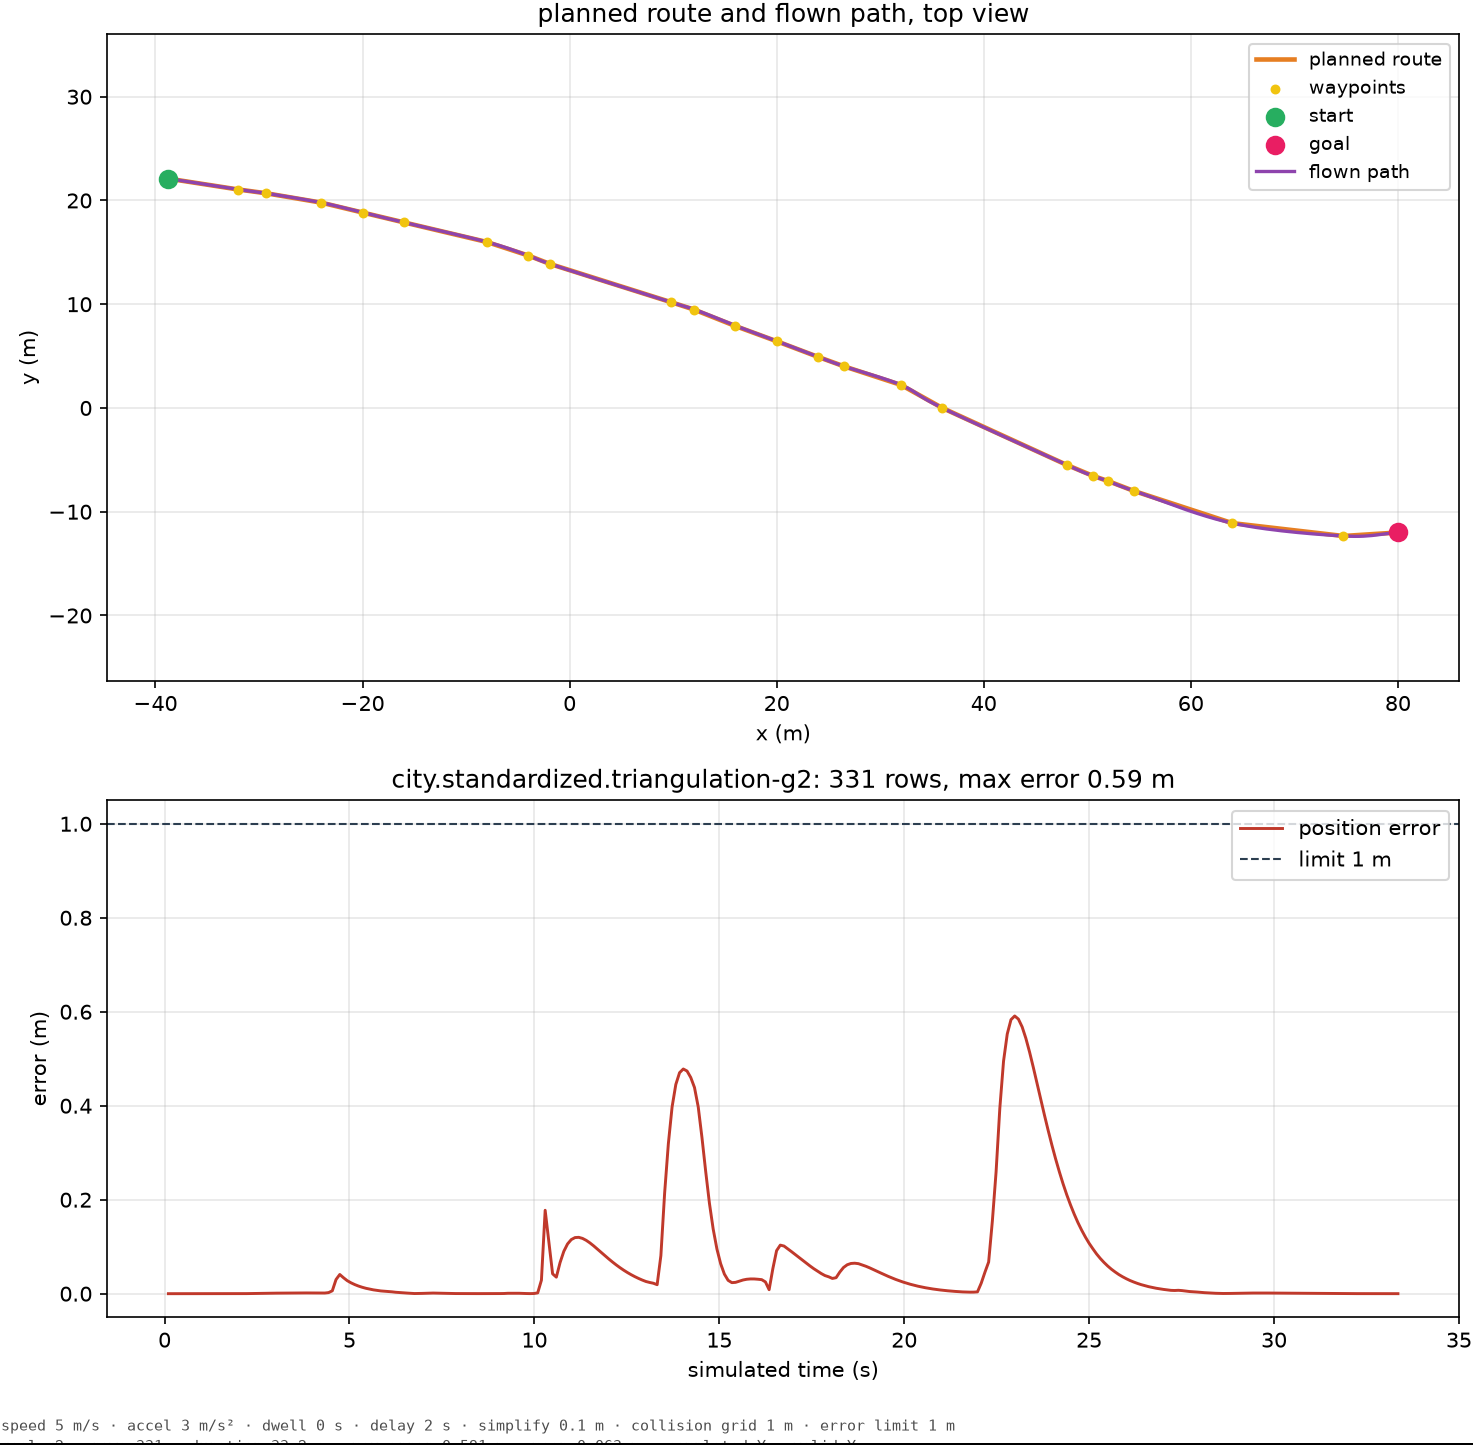
\includegraphics[width=\linewidth]{Figures/crop/cell4_g2_tracking.png}
    \caption{Lưới $4$, G2: $e_{\max}=0{,}591$, đạt mốc.}
  \end{subfigure}\par\vspace{2pt}
  \begin{subfigure}{0.66\textwidth}
    \centering
    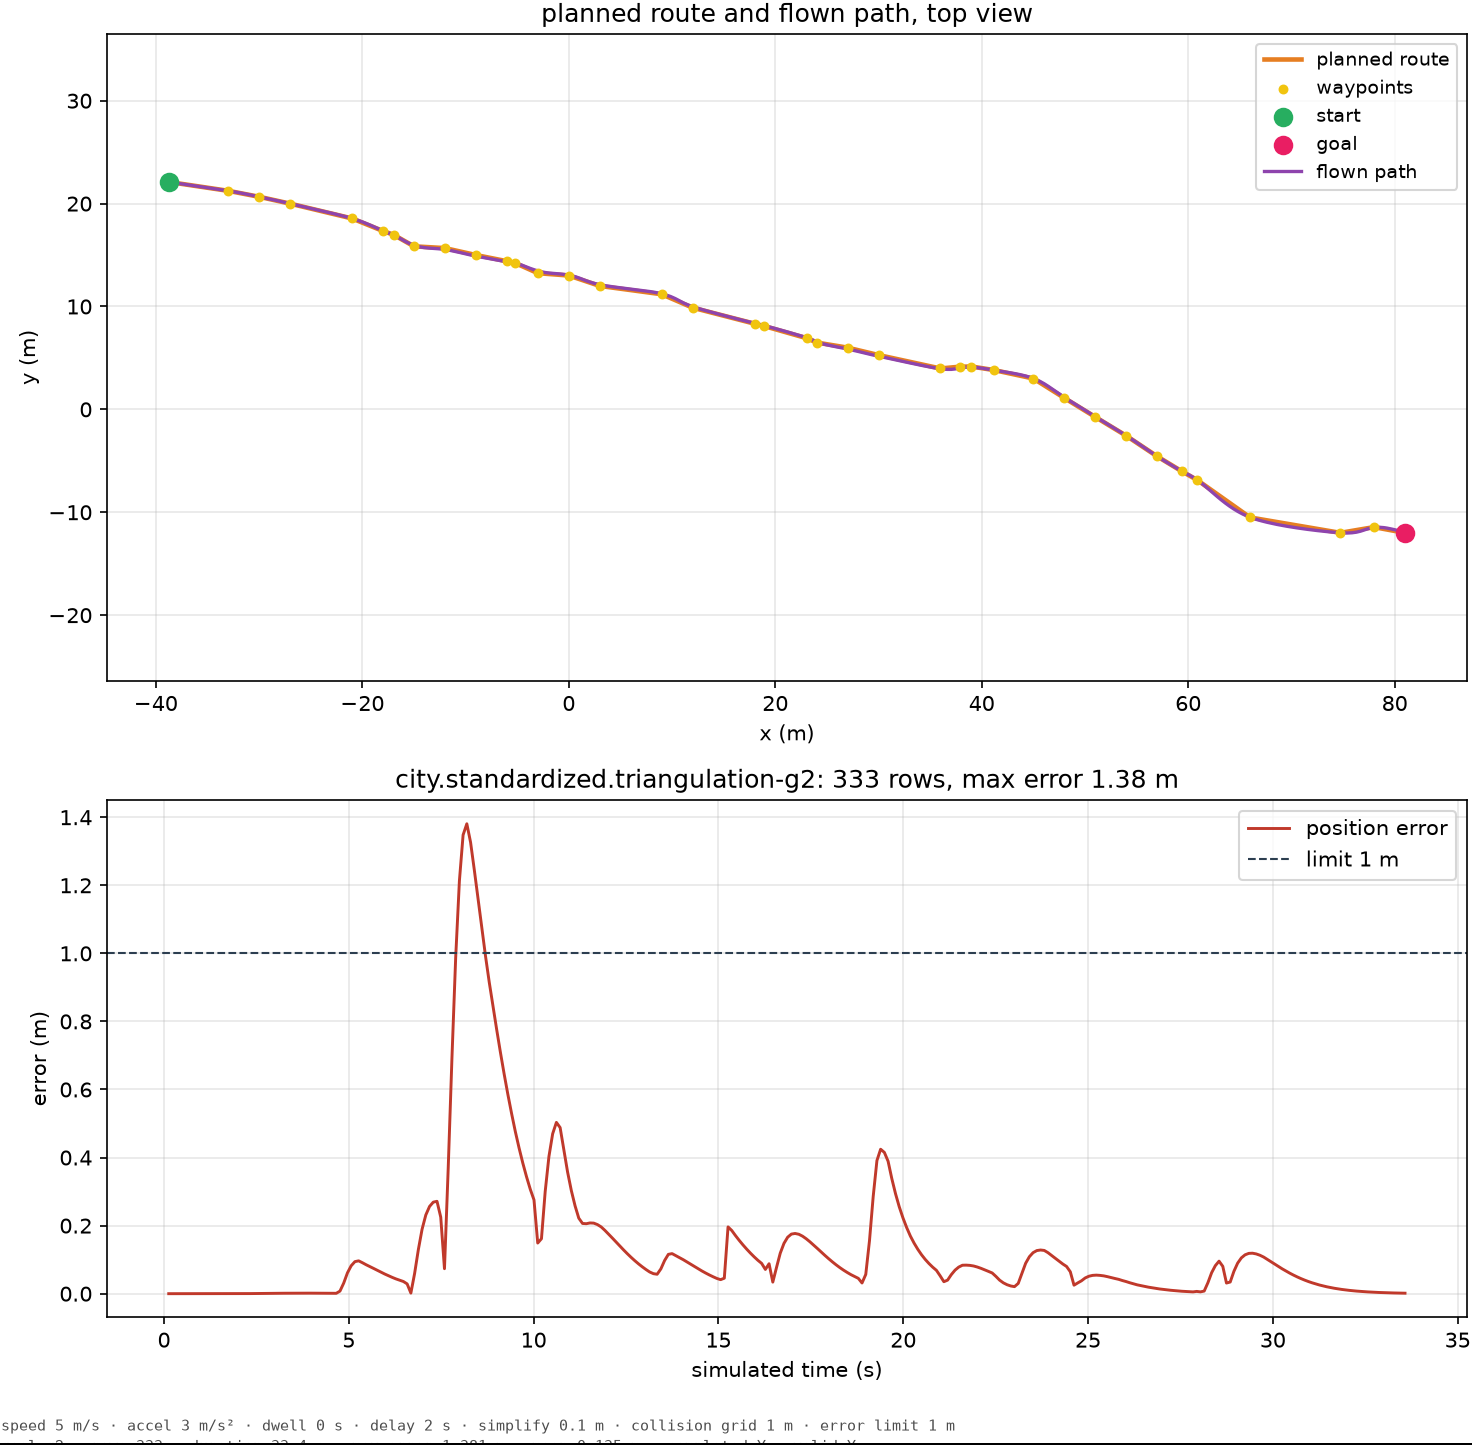
\includegraphics[width=\linewidth]{Figures/crop/cell3_g2_tracking.png}
    \caption{Lưới $3$, G2: $e_{\max}=1{,}381$, trượt mốc do sai số thẳng đứng.}
  \end{subfigure}
  \caption{Đường đã bay và sai số theo thời gian ở đích G2. Panel trên là mặt
    bằng tuyến kế hoạch (cam) và đường đã bay (tím); panel dưới là sai số, nét
    đứt là mốc $1$ đơn vị.}
  \label{fig:tracking}
\end{figure*}

Hình~\ref{fig:tracking} cho thấy đường bay gần như phủ lên tuyến kế hoạch ở
panel mặt bằng; khác biệt nằm ở panel sai số, nơi các đỉnh xuất hiện đúng tại các
góc cua. Với lưới $4$, đỉnh lớn nhất $0{,}591$ vẫn dưới mốc; với lưới $3$, đỉnh
$1{,}381$ vượt mốc và tập trung trong khoảng $7$--$9$ giây, đúng giai đoạn leo
vách dốc.

\begin{figure*}[!t]
  \centering
  \begin{subfigure}{0.66\textwidth}
    \centering
    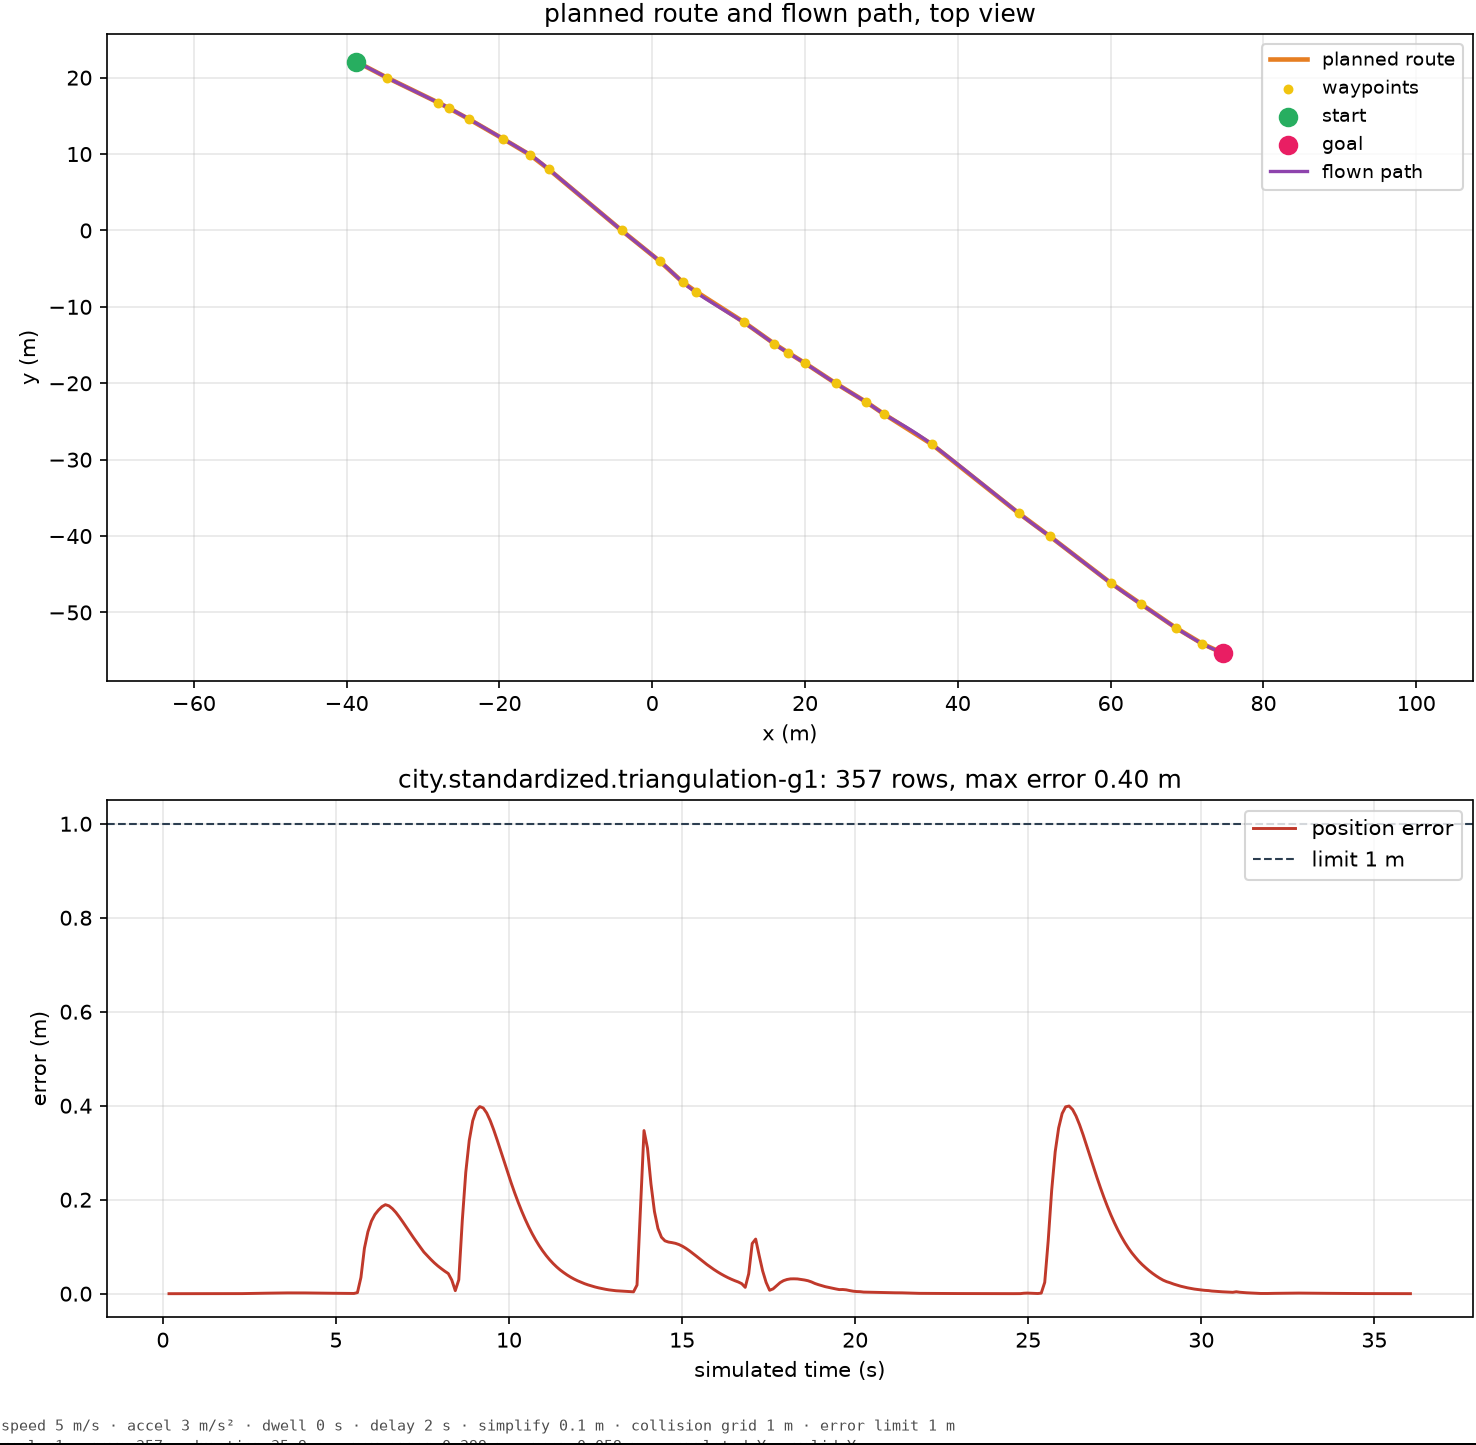
\includegraphics[width=\linewidth]{Figures/crop/cell4_g1_tracking.png}
    \caption{Lưới $4$, G1: $e_{\max}=0{,}399$, đạt mốc.}
  \end{subfigure}\par\vspace{2pt}
  \begin{subfigure}{0.66\textwidth}
    \centering
    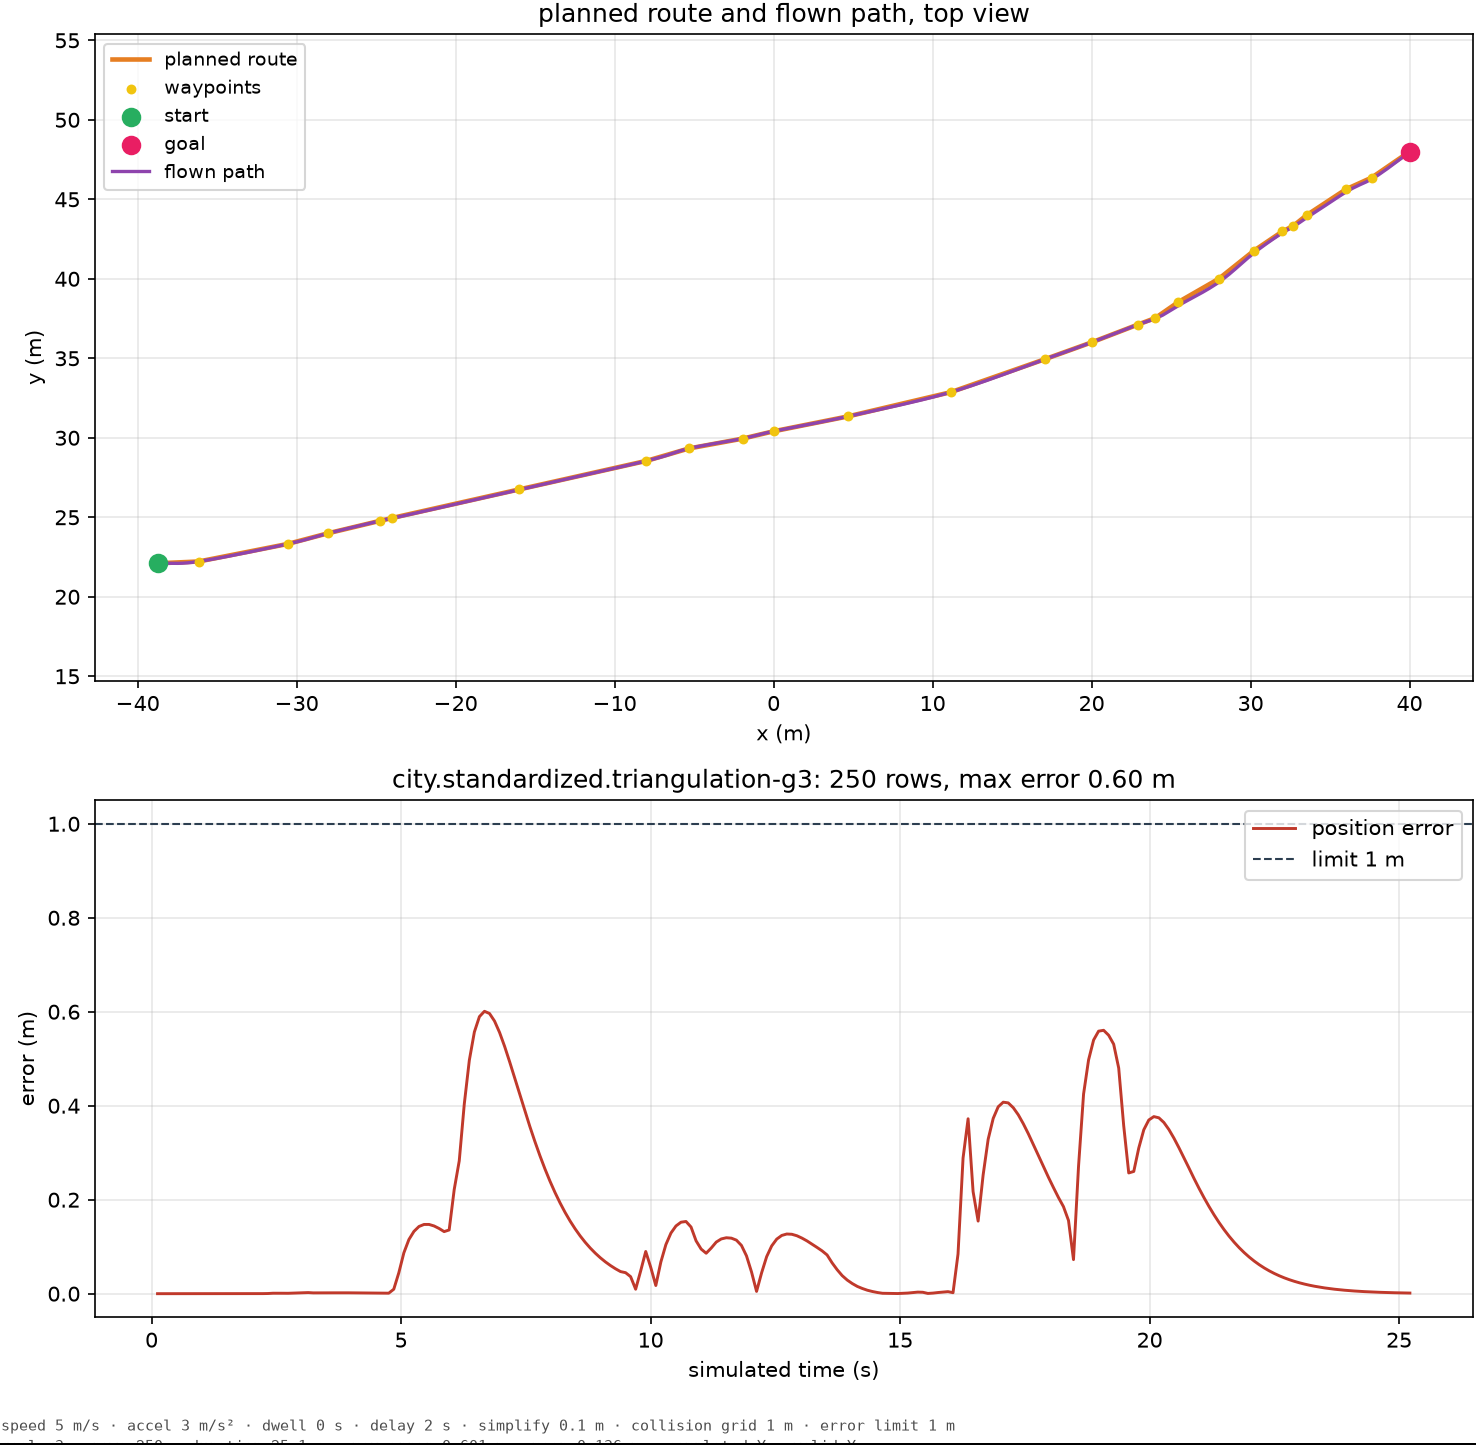
\includegraphics[width=\linewidth]{Figures/crop/cell4_g3_tracking.png}
    \caption{Lưới $4$, G3: $e_{\max}=0{,}601$, đạt mốc.}
  \end{subfigure}
  \caption{Đường đã bay và sai số của hai đích còn lại trên lưới $4$: G1 (trên)
    và G3 (dưới). Cả hai đều nằm dưới mốc $1$ đơn vị.}
  \label{fig:tracking-g1g3}
\end{figure*}

Hình~\ref{fig:tracking-g1g3} cho thấy G1 và G3 có cùng dạng sai số: gần như
phẳng trên đoạn thẳng, tăng ở các góc cua rồi giảm khi ra khỏi góc. G3 có nhiều
đỉnh hơn vì tuyến có nhiều waypoint và một đoạn ngắn $0{,}777$; đỉnh lớn nhất
$0{,}601$ vẫn dưới mốc. G1 có ít đỉnh hơn và sai số lớn nhất $0{,}399$, phù hợp
với khoảng cách waypoint đều hơn.

\begin{figure*}[!t]
  \centering
  \begin{subfigure}{0.45\textwidth}
    \centering
    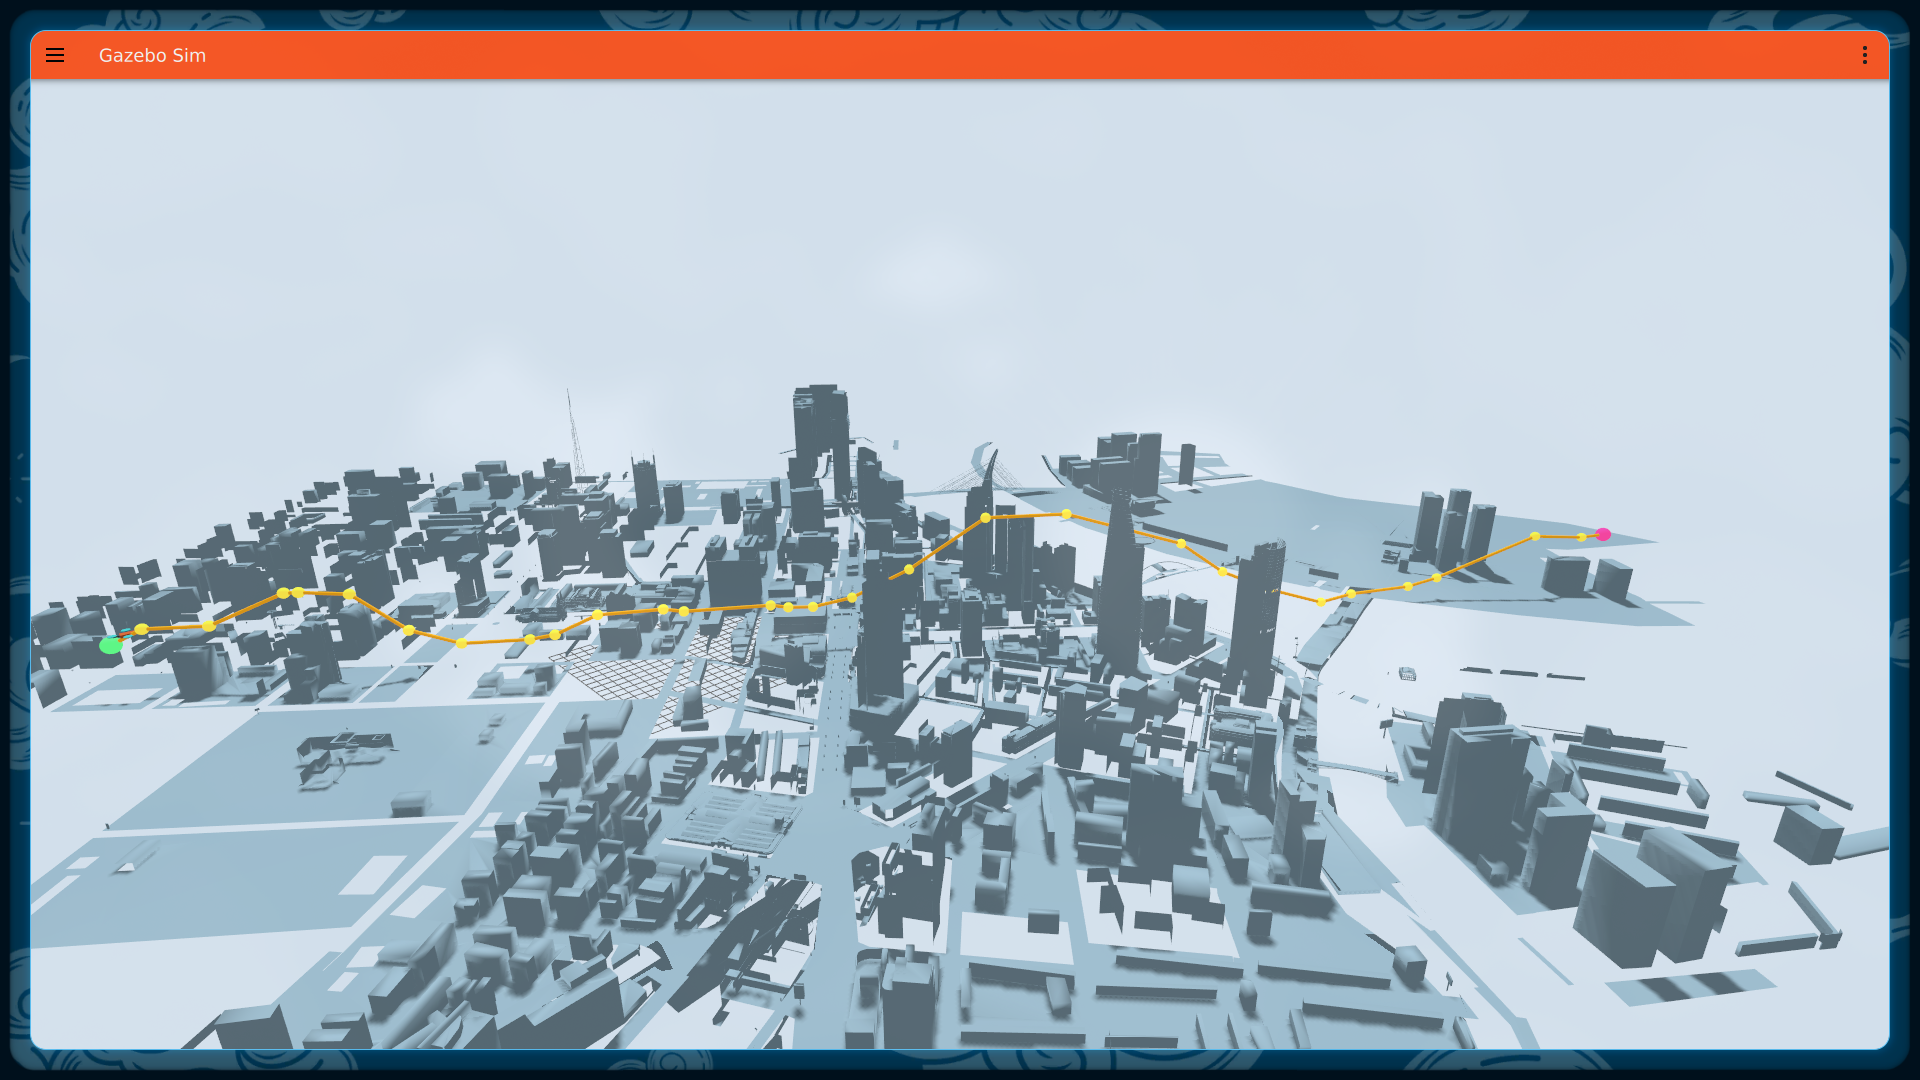
\includegraphics[width=\linewidth]{Figures/crop/gazebo_g1_city.png}
    \caption{G1, toàn cảnh.}
  \end{subfigure}\hfill
  \begin{subfigure}{0.45\textwidth}
    \centering
    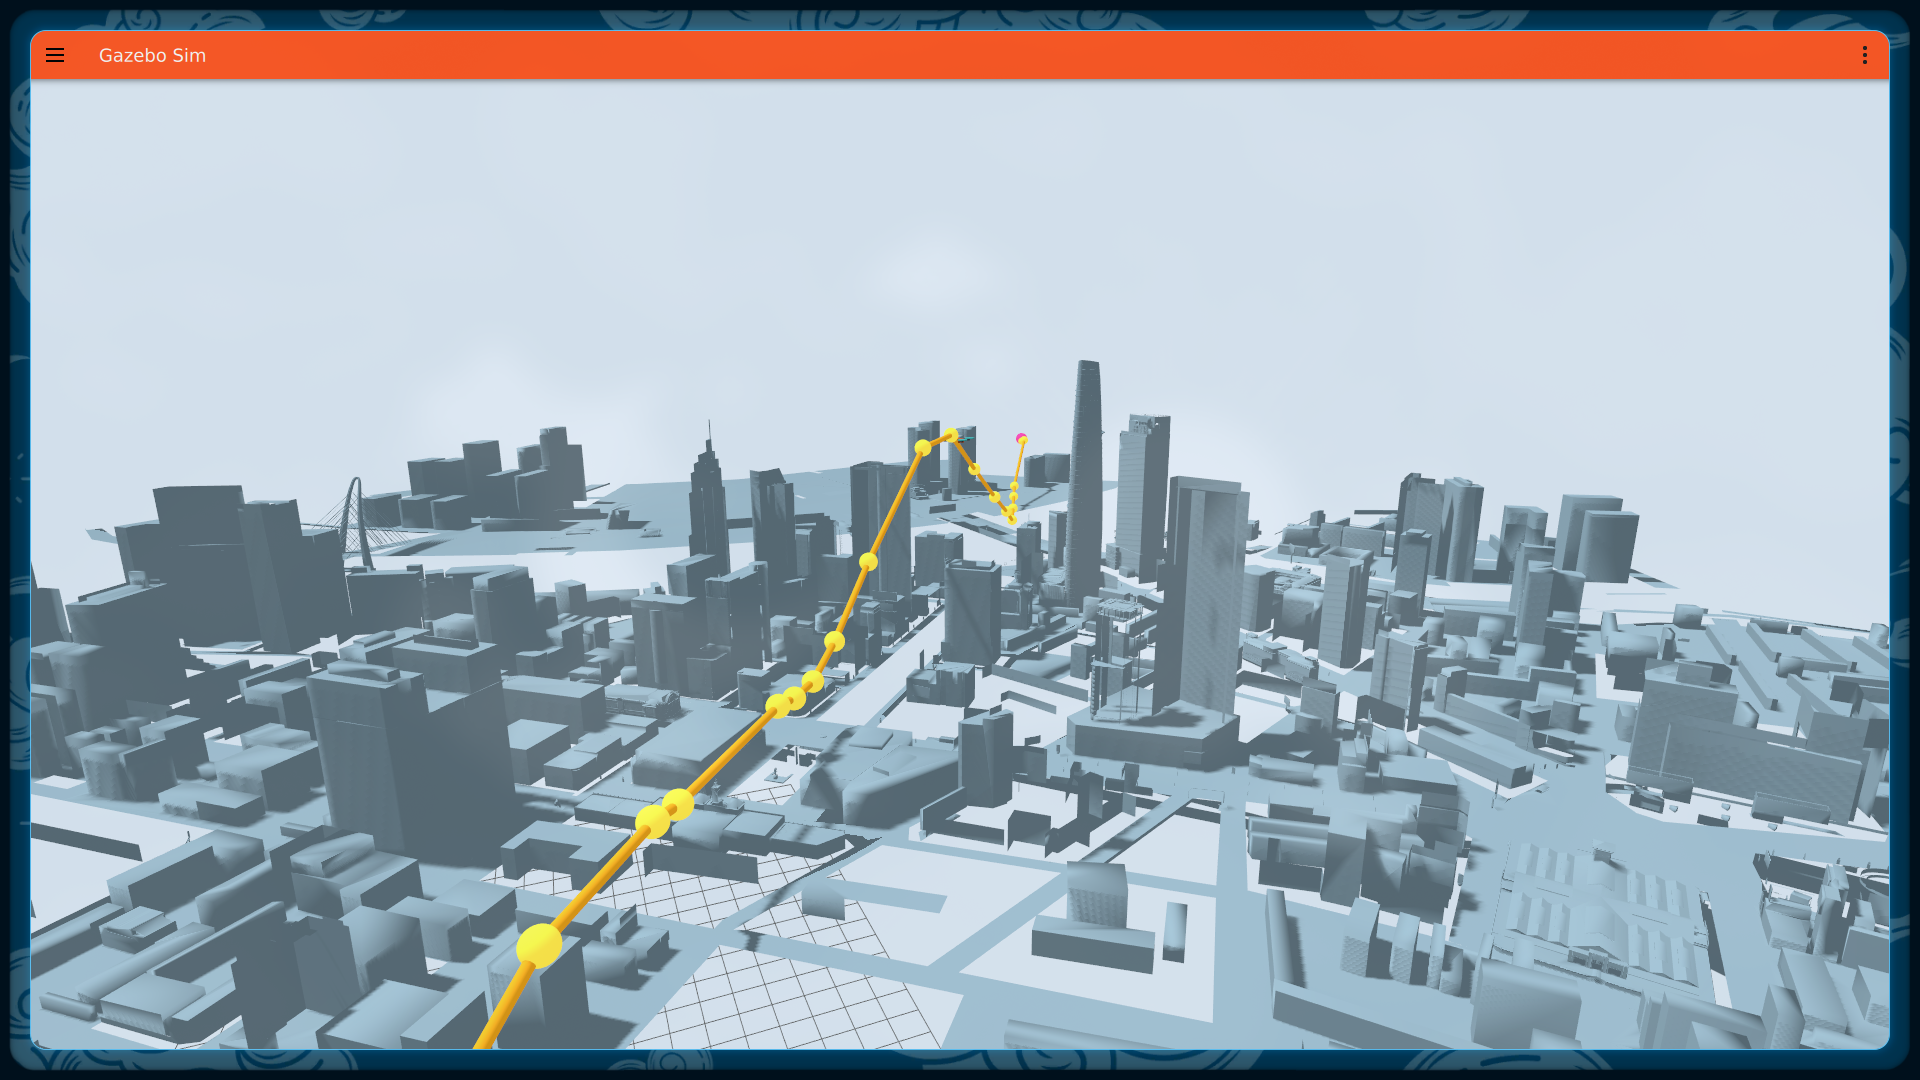
\includegraphics[width=\linewidth]{Figures/crop/gazebo_g1_close.png}
    \caption{G1, cận cảnh.}
  \end{subfigure}\par\vspace{2pt}
  \begin{subfigure}{0.45\textwidth}
    \centering
    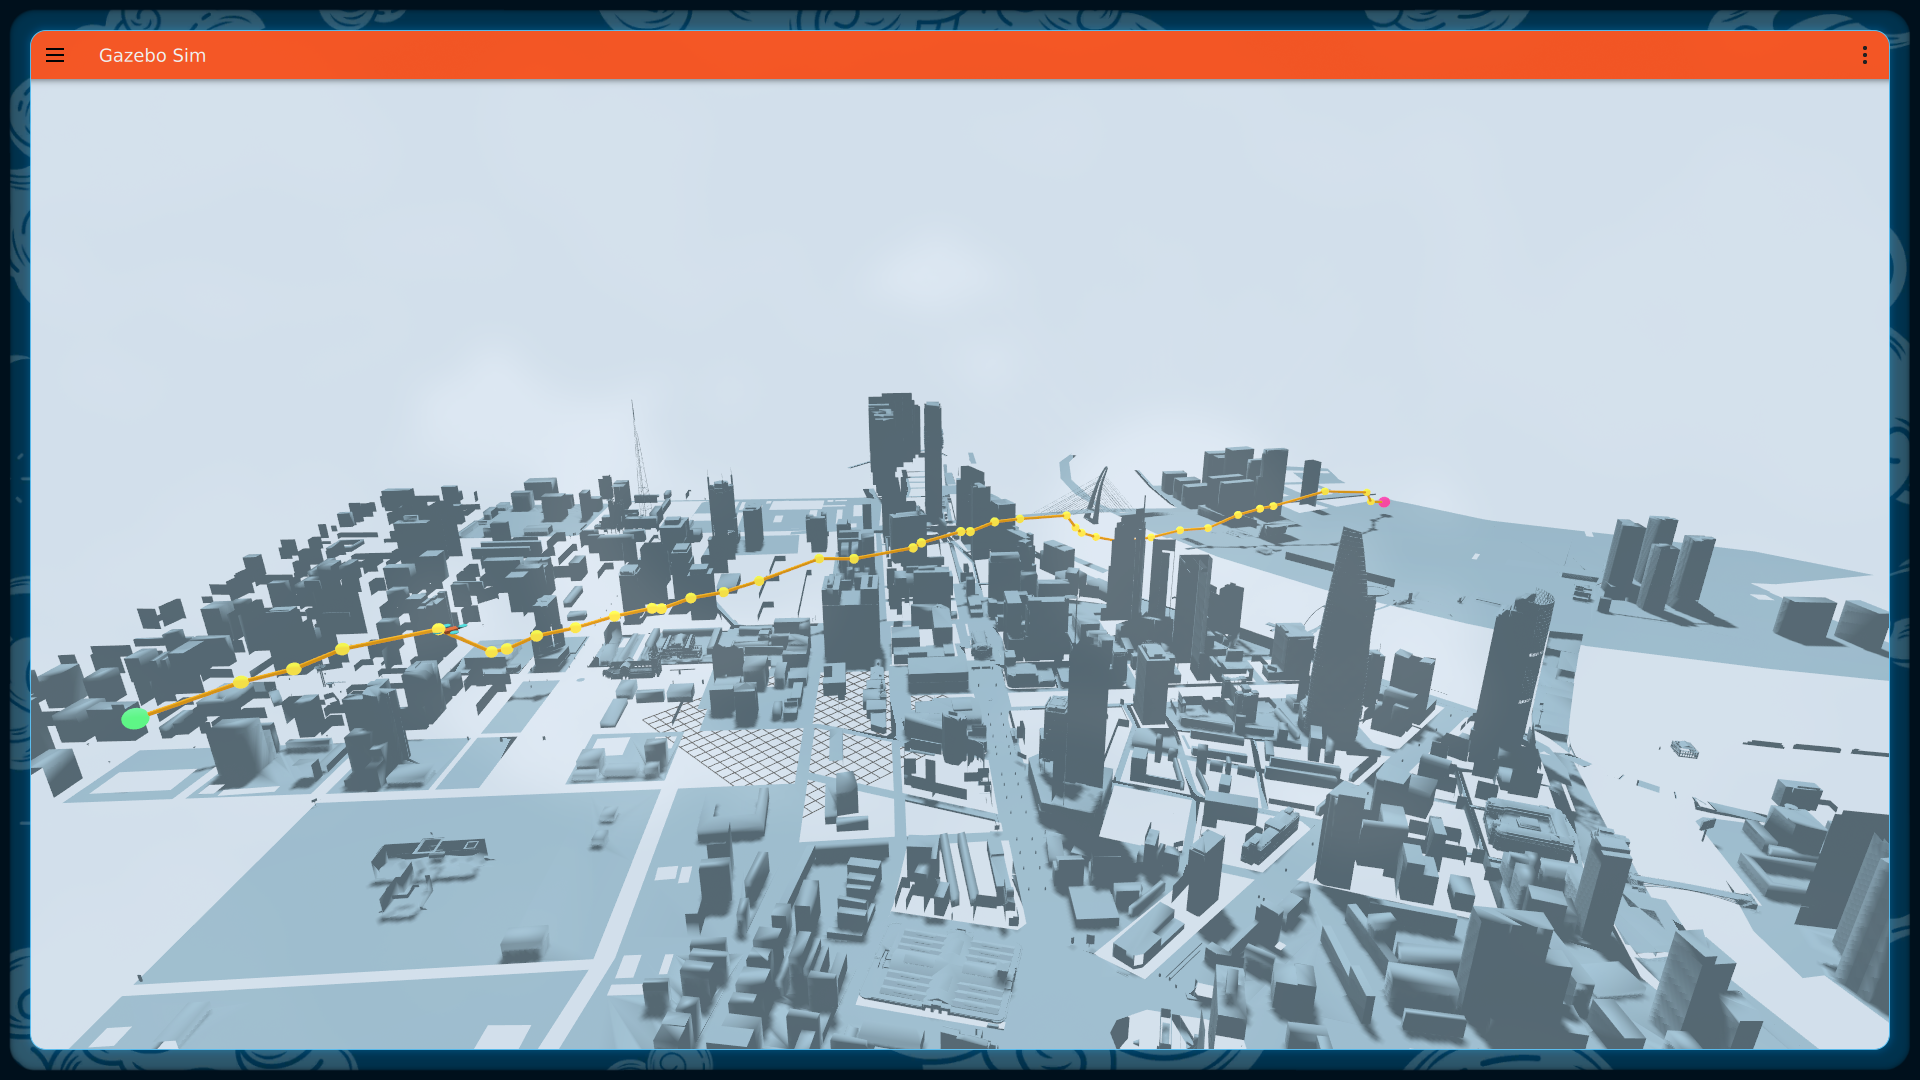
\includegraphics[width=\linewidth]{Figures/crop/gazebo_g2_city.png}
    \caption{G2, toàn cảnh.}
  \end{subfigure}\hfill
  \begin{subfigure}{0.45\textwidth}
    \centering
    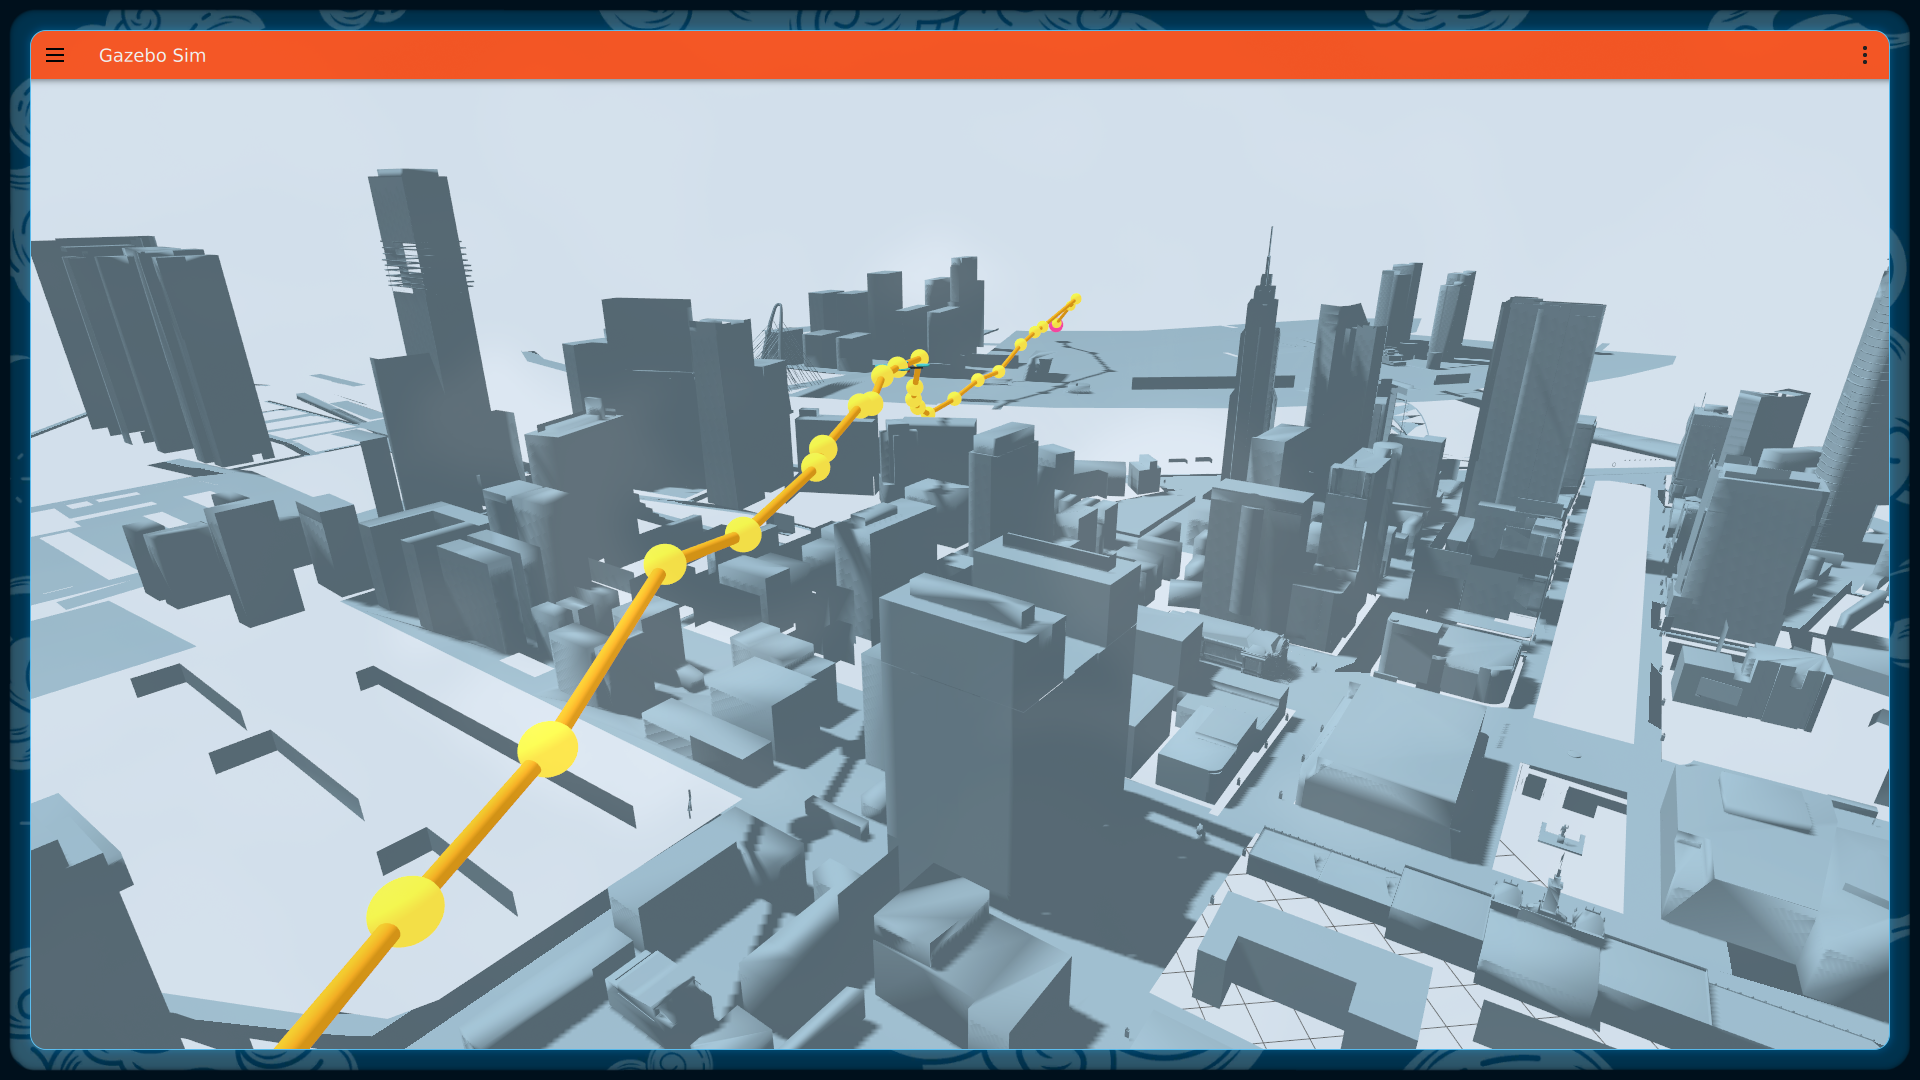
\includegraphics[width=\linewidth]{Figures/crop/gazebo_g2_close.png}
    \caption{G2, cận cảnh.}
  \end{subfigure}\par\vspace{2pt}
  \begin{subfigure}{0.45\textwidth}
    \centering
    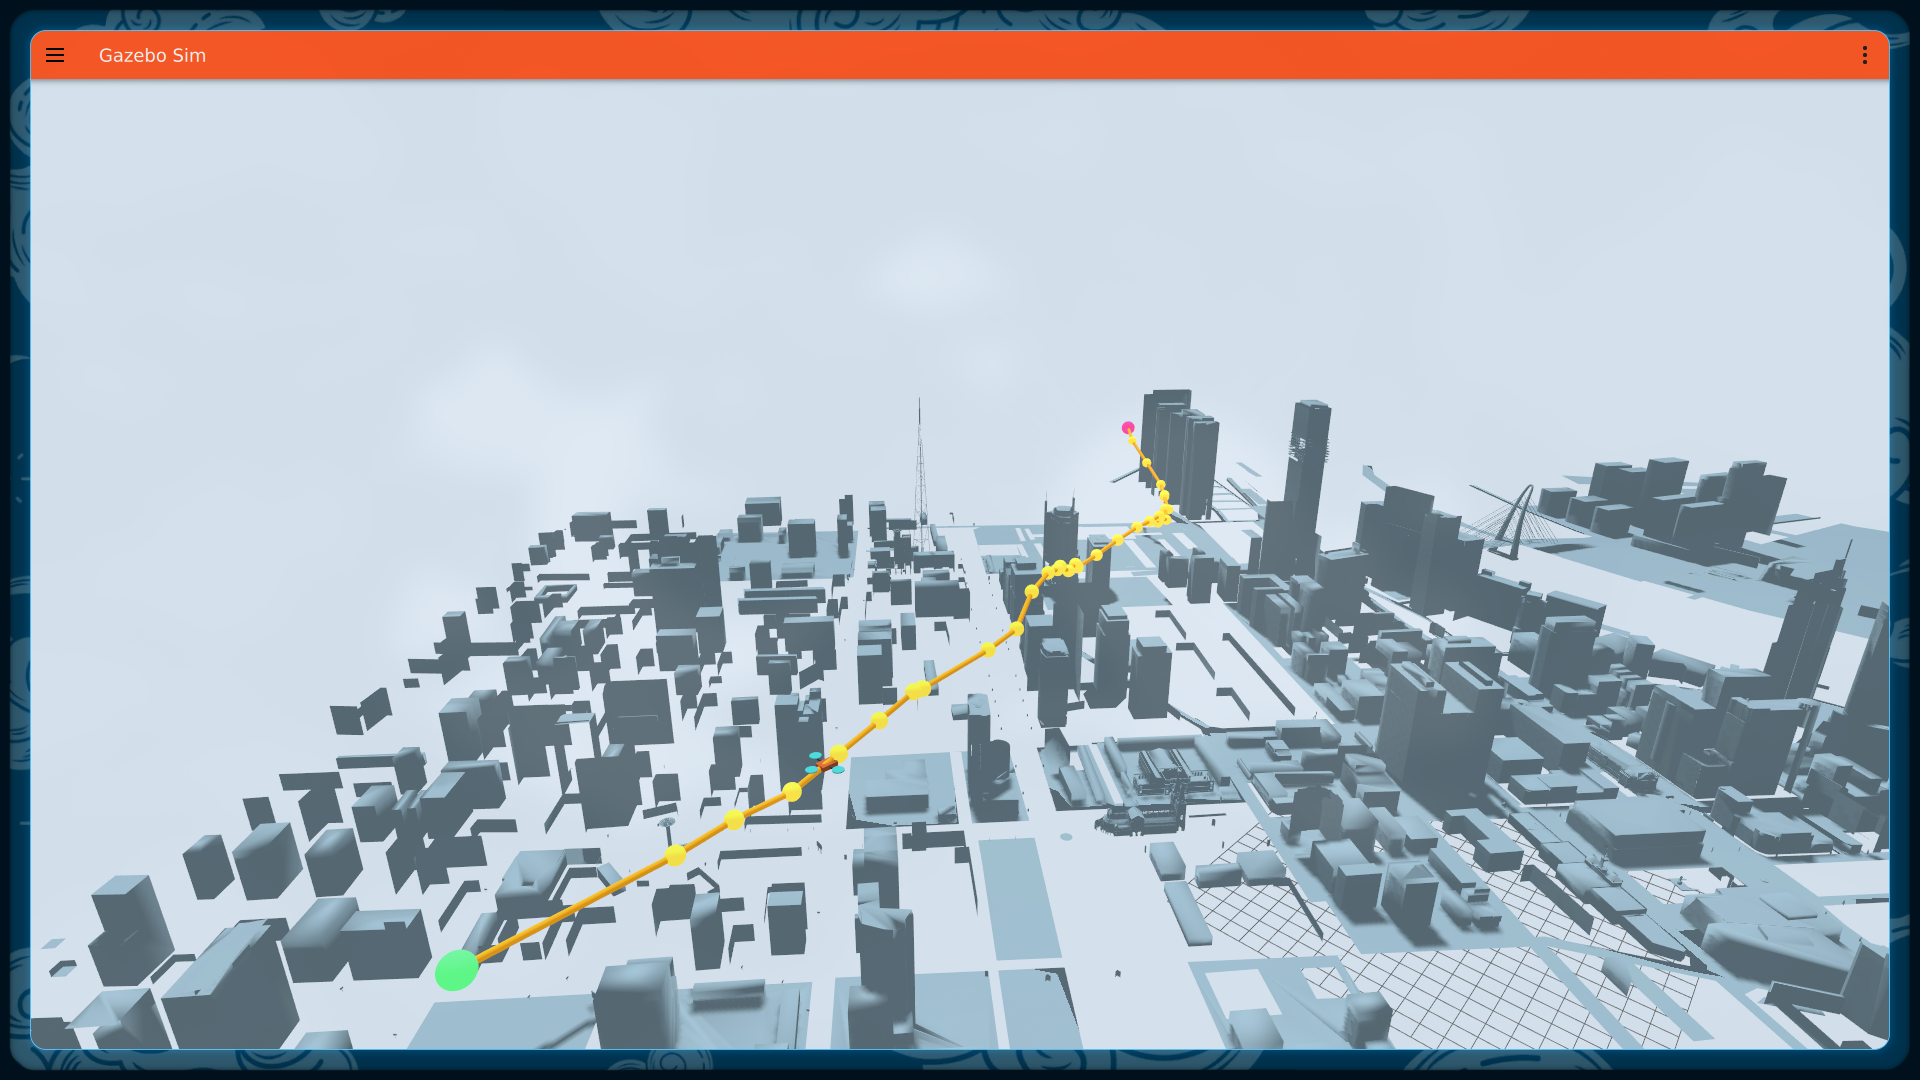
\includegraphics[width=\linewidth]{Figures/crop/gazebo_g3_city.png}
    \caption{G3, toàn cảnh.}
  \end{subfigure}\hfill
  \begin{subfigure}{0.45\textwidth}
    \centering
    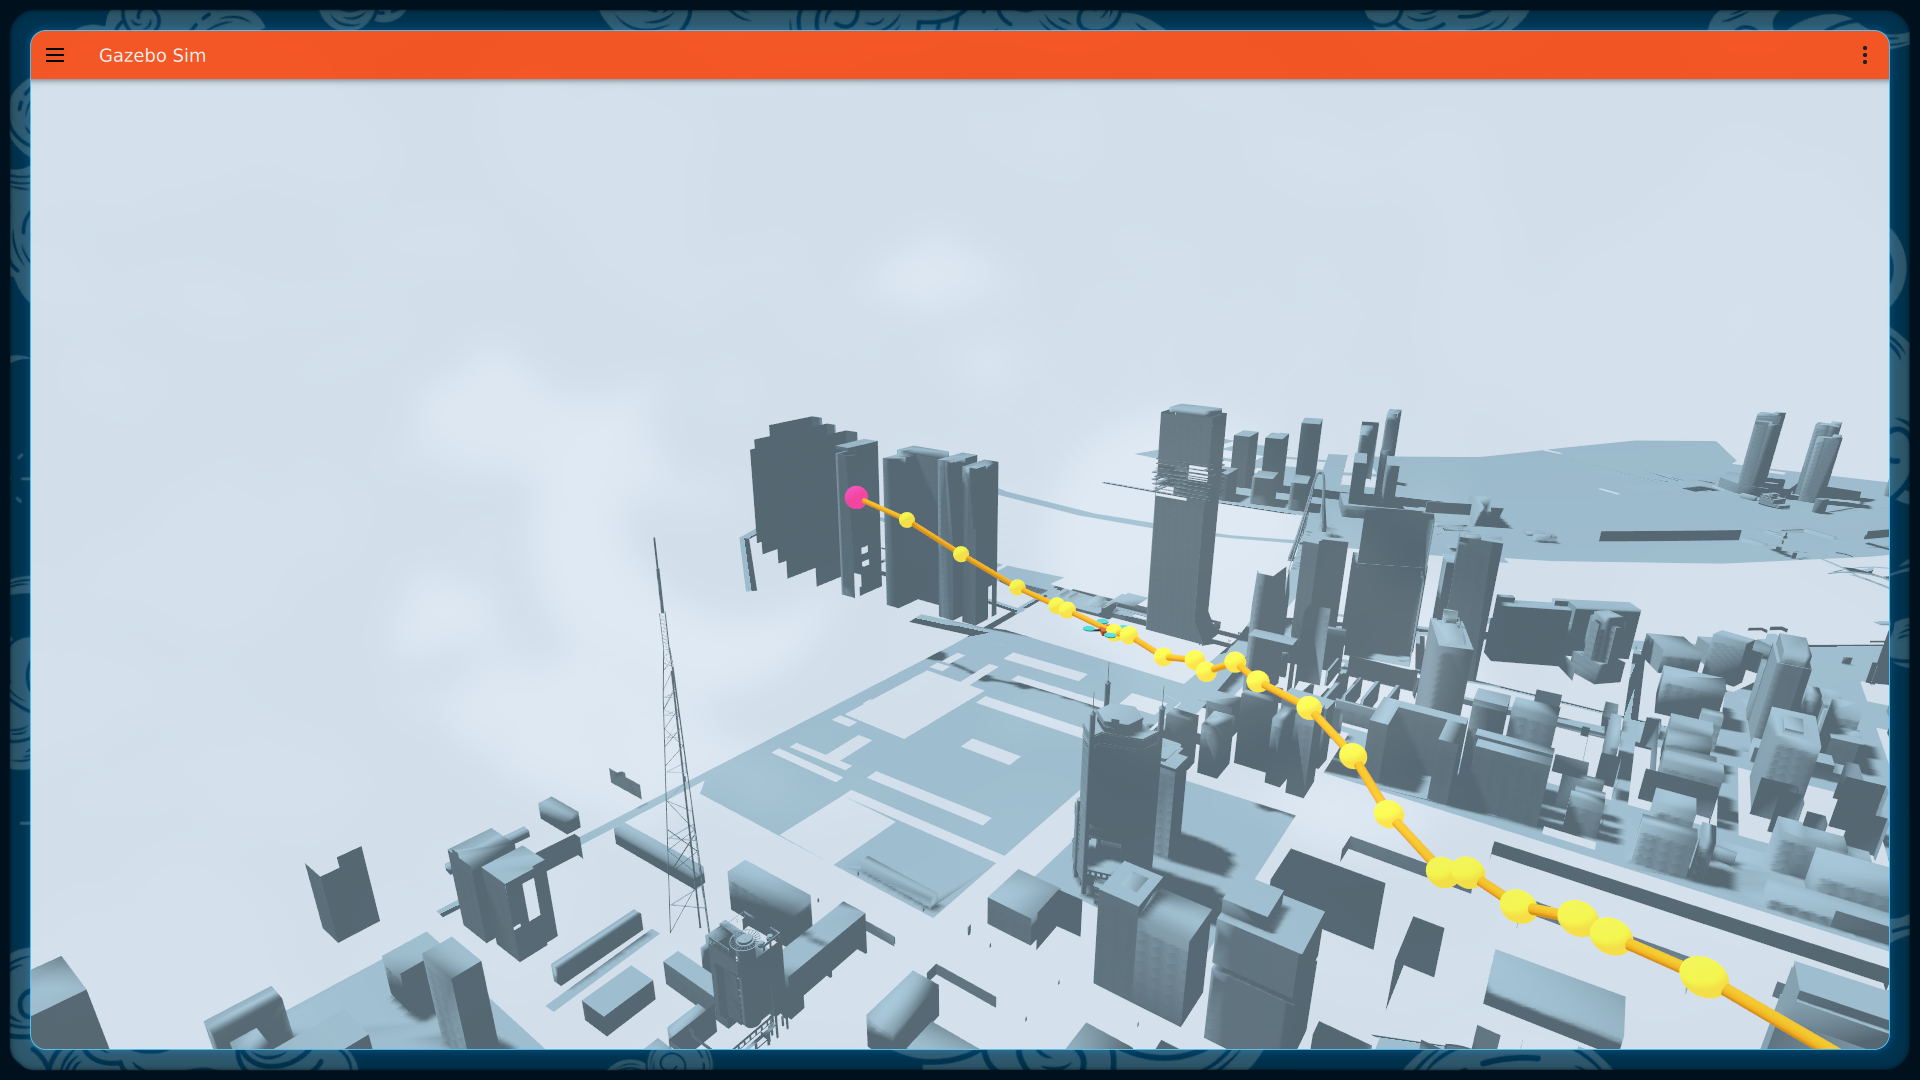
\includegraphics[width=\linewidth]{Figures/crop/gazebo_g3_close.png}
    \caption{G3, cận cảnh.}
  \end{subfigure}
  \caption{Giao diện Gazebo trong ba phiên G1, G2 và G3: thành phố, tuyến kế
    hoạch màu cam, waypoint vàng, điểm xuất phát xanh và đích hồng. Ảnh chụp
    giao diện chỉ để minh họa; kết luận định lượng lấy từ telemetry.}
  \label{fig:gazebo-g1}
\end{figure*}

Hình~\ref{fig:gazebo-g1} cho thấy cả ba tuyến đều đi qua các khe phố và bám theo
cao độ công trình; các waypoint vàng nằm trên mái hoặc sát mặt envelope, không đi
xuyên qua khối nhà. G1 đi gần như thẳng theo hướng đông-nam; G2 có một đoạn leo
lên tháp cao rồi xuống; G3 đi về phía đông-bắc và có nhiều đoạn đổi hướng hơn.
Các ảnh này chỉ minh họa giao diện, không dùng để đo sai số.

\begin{table*}[!t]
  \caption{Thống kê khoảng cách waypoint trên tuyến đã rút gọn mà plugin thực sự
    bay. $n$ là số waypoint; $d_{\min}$, $d_{\rm med}$, $d_{\max}$ là khoảng cách
    đoạn ngắn nhất, trung vị và dài nhất; $r_{\max}$ là tỉ lệ lớn nhất giữa độ dài
    tiếp tuyến Catmull--Rom và đoạn ngắn kề nó.}
  \label{tab:waypoints}
  {\fontsize{7}{8.6}\selectfont
  \begin{adjustbox}{max width=\textwidth}
  \begin{tabular}{@{}llrrrrr@{}}
    \toprule
    Cấu hình & Goal & $n$ & $d_{\min}$ & $d_{\rm med}$ & $d_{\max}$ & $r_{\max}$ \\
    \midrule
    lưới $5$ & g1 & 27 & 1,389 & 5,633 & 12,766 & 3,36 \\
             & g2 & 25 & 1,264 & 3,705 & 19,464 & 7,60 \\
             & g3 & 24 & 1,217 & 3,533 & 10,347 & 1,65 \\
    \midrule
    lưới $4$ & g1 & 27 & 1,595 & 4,804 & 15,624 & 2,92 \\
             & g2 & 24 & 1,545 & 4,431 & 13,600 & 3,15 \\
             & g3 & 26 & 0,777 & 2,935 &  8,208 & 5,40 \\
    \midrule
    lưới $3$ & g1 & 30 & 1,119 & 4,925 & 11,887 & 3,24 \\
             & g2 & 38 & 0,801 & 3,102 &  8,988 & 3,62 \\
             & g3 & 33 & 0,776 & 2,783 &  8,760 & 4,40 \\
    \bottomrule
  \end{tabular}
  \end{adjustbox}}
\end{table*}

\begin{table*}[!t]
  \caption{Phân rã sai số tại một số thời điểm của G2 trên lưới $3$. $z$ và
    $z_{\rm ref}$ là cao độ đo và cao độ tham chiếu; $\Delta z$ là thành phần
    đứng; tỉ lệ đứng là $|\Delta z|/e$.}
  \label{tab:g2vertical}
  {\fontsize{7}{8.6}\selectfont
  \begin{tabular}{@{}rrrrrrrr@{}}
    \toprule
    $t$ (s) & $z$ & $z_{\rm ref}$ & $\Delta z$ & $e$ & Tỉ lệ đứng
      & $v_z$ & $v_{z,\rm ref}$ \\
    \midrule
    7,285 & 7,032 & 6,765 & $+0{,}268$ & 0,269 & 99,6\,\% & $-3{,}498$ & $-3{,}569$ \\
    7,891 & 5,668 & 6,648 & $-0{,}980$ & 0,987 & 99,3\,\% & $-0{,}530$ & $+2{,}083$ \\
    8,092 & 5,678 & 7,017 & $-1{,}339$ & 1,348 & 99,4\,\% & $+0{,}524$ & $+1{,}383$ \\
    8,193 & 5,741 & 7,115 & $-1{,}374$ & 1,381 & 99,5\,\% & $+0{,}682$ & $+0{,}537$ \\
    8,294 & 5,806 & 7,129 & $-1{,}323$ & 1,326 & 99,7\,\% & $+0{,}560$ & $-0{,}164$ \\
    \bottomrule
  \end{tabular}}
\end{table*}

Không có cấu hình nào nhỏ nhất ở mọi đích: lưới $5$ có sai số G1 thấp nhất
($0{,}365$), lưới $3$ có sai số G3 thấp nhất ($0{,}580$), còn lưới $4$ chỉ nhỉnh
hơn ở hai đích này nhưng là cấu hình duy nhất đạt mốc ở cả ba. Vì vậy nên đọc kết
quả theo tiêu chí đã đặt trước (đạt $1$ đơn vị ở mọi đích) thay vì chọn cấu hình
theo một con số sai số đơn lẻ.

\subsection{So sánh ba cấu hình và tái lập}\label{sec:archive}

Ba cấu hình được lưu thành ba bộ kết quả độc lập, không ghi đè lên nhau. Mỗi bộ
gồm bề mặt, route, world, telemetry, ảnh và một bản kê khai tham số cùng SHA của
mọi tệp. Nhờ vậy có thể so sánh sau khi lần chạy mới nhất đã thay đổi thư mục làm
việc. Bảng~\ref{tab:summary} tóm tắt ba cấu hình; Hình~\ref{fig:routes} so sánh
tuyến trên lưới $4$ và lưới $3$.

\begin{table*}[!t]
  \caption{Tóm tắt ba cấu hình: kích thước lưới, thời gian lập tuyến, số lần lan
    truyền, sai số lớn nhất từng đích và số đích đạt mốc $1$.}
  \label{tab:summary}
  {\fontsize{7}{8.6}\selectfont
  \begin{adjustbox}{max width=\textwidth}
  \begin{tabular}{@{}lrrrrrrl@{}}
    \toprule
    Cấu hình & $V/F$ & $T_{\rm plan}$ (s) & $\sum P$
      & $e_{\max}$ G1 & $e_{\max}$ G2 & $e_{\max}$ G3 & Đạt mốc \\
    \midrule
    lưới $5$ & 2\,295/4\,400 & 44,984 & 104 & 0,365 & 1,022 & 0,852 & 2/3 \\
    lưới $4$ & 3\,355/6\,480 & 186,175 & 187 & 0,399 & 0,591 & 0,601 & 3/3 \\
    lưới $3$ & 5\,913/11\,520 & 1\,008,389 & 429 & 0,508 & 1,381 & 0,580 & 2/3 \\
    \bottomrule
  \end{tabular}
  \end{adjustbox}}
\end{table*}

\begin{figure*}[!t]
  \centering
  \begin{subfigure}{0.70\textwidth}
    \centering
    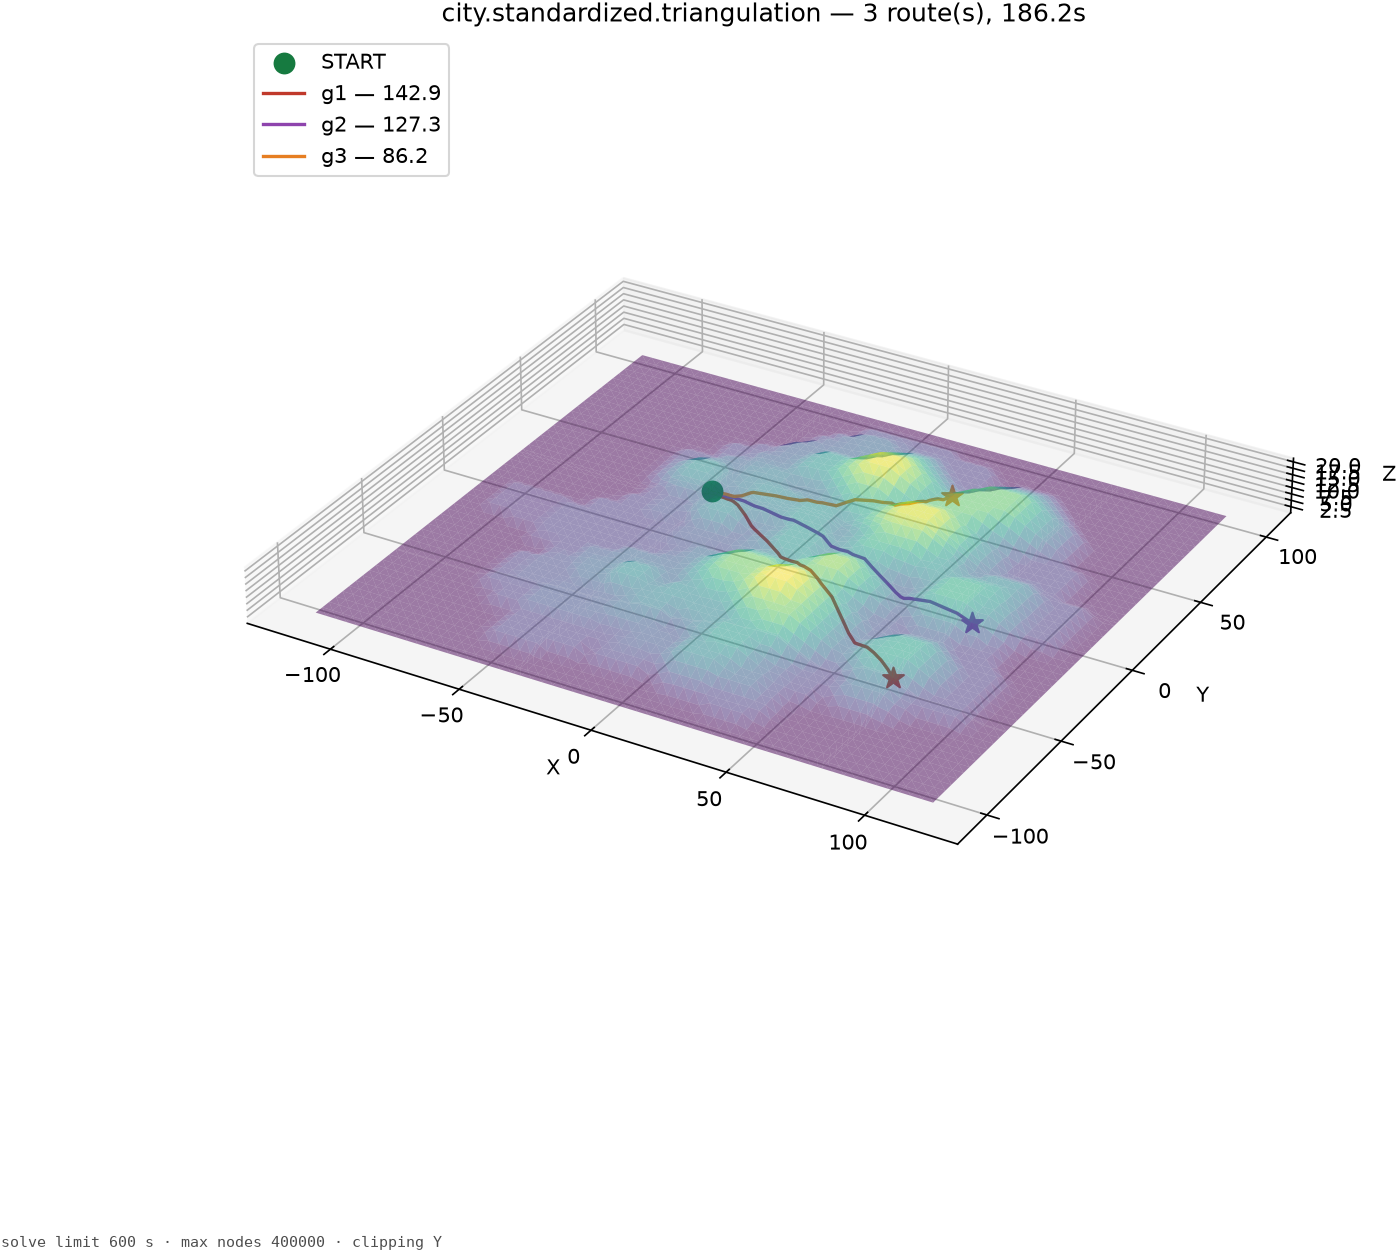
\includegraphics[width=\linewidth]{Figures/crop/cell4_routes.png}
    \caption{Lưới $4$: G1 $142{,}909050$, G2 $127{,}295935$, G3 $86{,}194146$.}
  \end{subfigure}\par\vspace{2pt}
  \begin{subfigure}{0.70\textwidth}
    \centering
    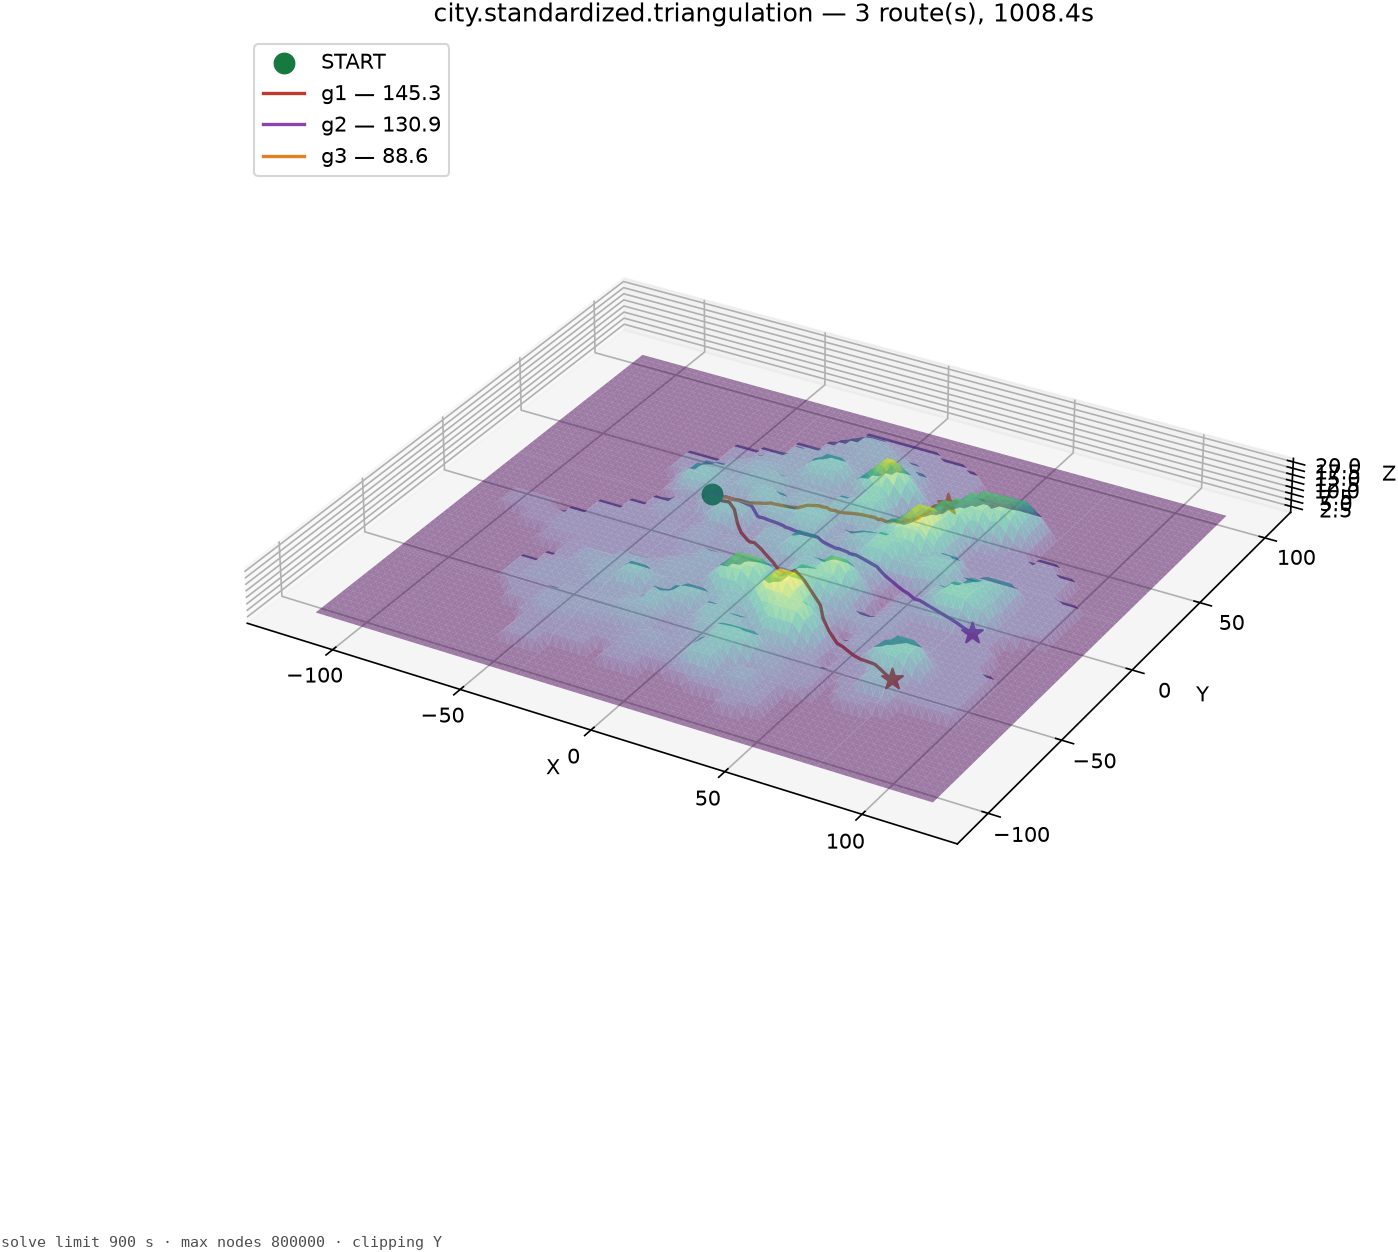
\includegraphics[width=\linewidth]{Figures/crop/cell3_routes.png}
    \caption{Lưới $3$: G1 $145{,}314559$, G2 $130{,}891670$, G3 $88{,}611502$.}
  \end{subfigure}
  \caption{Ba tuyến trên hai bề mặt. Lưới $4$ (trên) là cấu hình duy nhất đạt mốc
    bám tuyến $1$ ở cả ba đích; lưới $3$ (dưới) có bề mặt sát hình học hơn và
    tuyến dài hơn.}
  \label{fig:routes}
\end{figure*}

Hình~\ref{fig:routes} so sánh trực tiếp hai bề mặt. Ba tuyến trên lưới $3$ dài
hơn tuyến tương ứng trên lưới $4$ khoảng $2{,}4$; $3{,}6$ và $2{,}4$ đơn vị, trong
khi hình dạng tổng thể vẫn tương tự: cùng xuất phát từ một nguồn, cùng ba hướng
đích, nhưng lưới $3$ bám sát khối công trình hơn nên có thêm các đoạn lượn và
điểm đích bị snap xa hơn. Đây là lý do không thể quy toàn bộ chênh lệch độ dài
cho kích thước ô.

Hình~\ref{fig:routes-detail} cho thấy tuyến không đi theo mặt phẳng: khi bề mặt
có một tháp cao, tuyến leo lên theo ramp rồi xuống phía bên kia; các đoạn gãy
tương ứng với cạnh tam giác. Hình chiếu bằng xác nhận ba tuyến tách nhau ngay sau
nguồn và chỉ gặp lại ở vùng gần đích, phù hợp với việc mỗi goal được tìm trong
một lượt riêng.

\begin{figure*}[!t]
  \centering
  \begin{subfigure}{0.48\textwidth}
    \centering
    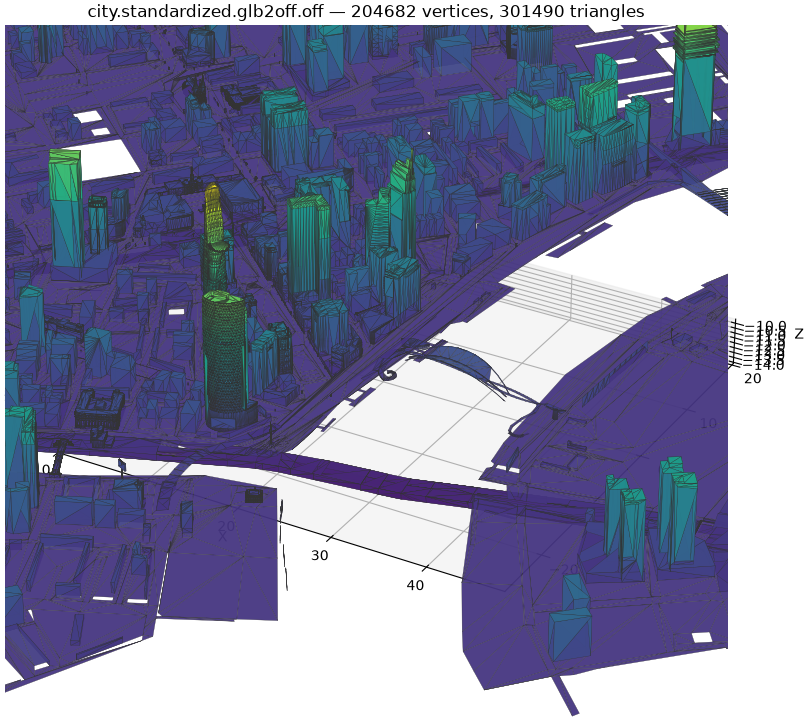
\includegraphics[width=\linewidth]{Figures/crop/etc_city_wide.png}
    \caption{Toàn cảnh vùng trung tâm.}
  \end{subfigure}\hfill
  \begin{subfigure}{0.48\textwidth}
    \centering
    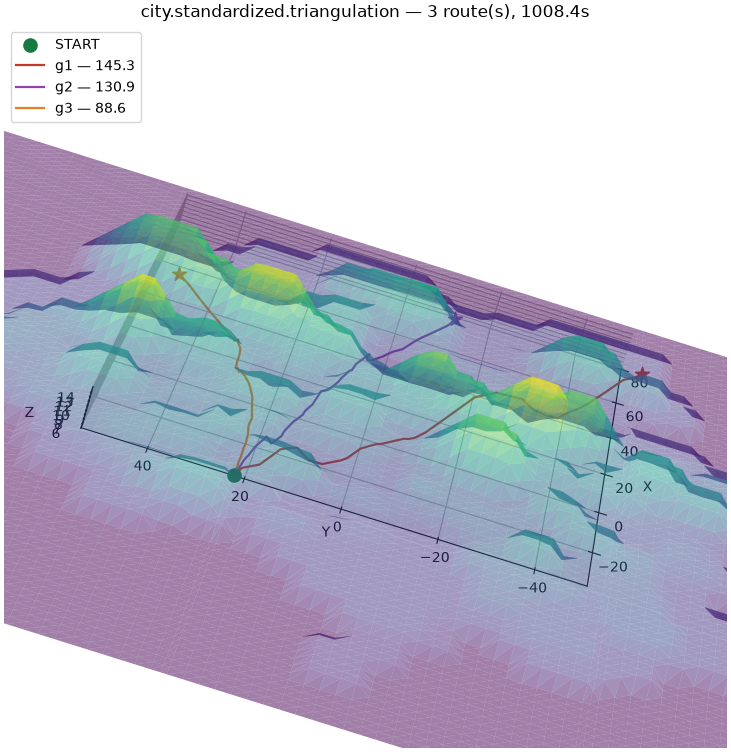
\includegraphics[width=\linewidth]{Figures/crop/etc_routes_3d_alt.png}
    \caption{Góc nhìn 3D khác của ba tuyến.}
  \end{subfigure}
  \caption{Hai góc nhìn bổ sung: toàn cảnh vùng trung tâm và một góc 3D khác của
    ba tuyến trên bề mặt lưới $3$ m.}
  \label{fig:extra-views}
\end{figure*}

Hình~\ref{fig:extra-views} cho thấy cùng một dữ liệu nhưng ở hai tỉ lệ: toàn cảnh
giúp thấy tuyến đi qua các khu phố khác nhau, còn góc 3D thứ hai làm rõ các đoạn
leo dốc và đổi hướng. Cả hai đều củng cố nhận xét rằng tuyến không đi theo mặt
phẳng và phải bám theo envelope.

\subsection{Những kết luận rút ra từ toàn bộ quy trình}\label{sec:lessons}

Sau khi chạy trọn quy trình từ scene thô đến telemetry, có thể rút ra sáu kết
luận vận hành, bên cạnh các số liệu ở trên.

\begin{enumerate}
  \item \textbf{Quy trình ba giai đoạn là một chuỗi kiểm chứng, không chỉ là ba
    lệnh.} Mỗi giai đoạn ghi hash của đầu vào và đầu ra; bộ kết quả lưu cả bản kê
    khai. Nhờ đó một con số trong bài truy ngược được về đúng scene, bề mặt,
    mission, route và telemetry. Đây là điều kiện cần để kết quả mô phỏng được
    xem là bằng chứng, không chỉ là ảnh minh họa.
  \item \textbf{Chọn kích thước ô là bài toán cân bằng, không phải ``càng mịn càng
    tốt''.} Lưới $5$ m đủ nhanh nhưng waypoint không đều ở G2; lưới $4$ m là cấu
    hình duy nhất đạt mốc $1$ ở cả ba đích; lưới $3$ m sát hình học hơn nhưng tạo
    vách $45^\circ$ và có sai số bám tại G2 chủ yếu theo phương
    thẳng đứng. Trong ba cấu hình đã chạy, $4$ m là lựa chọn
    làm việc; với lưới $3$ m, cần thử nghiệm giảm tốc độ hoặc
    làm mượt vùng chuyển tiếp cao độ trước khi đánh giá lại.
  \item \textbf{Sai số bám tuyến phải đo từ telemetry động.} Sai số tái dựng route
    ngoại tuyến chỉ phản ánh khâu dựng polyline, không phải sai số bám setpoint.
    Telemetry trong nghiên cứu cho $0{,}365$--$1{,}381$ mét; đây là đại lượng dùng
    để kết luận về chất lượng bay.
  \item \textbf{Không có bộ giải độc lập cho bề mặt thành phố.} Năm mesh nhỏ có
    tham chiếu và khớp $76/76$ đỉnh; bề mặt thành phố không có, nên bài không
    tuyên bố tuyến thành phố là tối ưu. Muốn kết luận mạnh hơn phải thêm một bộ
    giải trắc địa độc lập trên chính bề mặt đó.
  \item \textbf{Chi phí lập tuyến tăng nhanh hơn số tam giác.} Từ $4\,400$ lên
    $11\,520$ tam giác, số lần lan truyền tăng $104\to429$ và thời gian tăng
    $45\to1\,008$ giây. Với lưới mịn hơn nữa, cần tối ưu lan truyền hoặc chấp nhận
    chạy ngoại tuyến; không nên đặt quy trình tương tác trên cấu hình $3$ m hiện tại.
  \item \textbf{Giới hạn của mô hình phải được nói cùng kết quả.} Mô hình là khối
    điểm $1$ kg có PD, không có rotor, autopilot hay nhiễu; bề mặt là trường cao
    độ, không có mái nhô. Kết quả xác nhận tuyến khả thi trong mô hình rút gọn,
    không xác nhận khả năng bay thực. Các kết luận về G2 và về kích thước ô chỉ
    đúng trong phạm vi một mission, ba goal và một lần chạy mỗi cấu hình.
\end{enumerate}

\subsection{Thảo luận và giới hạn}\label{sec:gazebo-limits}

Ba cấu hình không phải một phép khảo sát riêng kích thước ô: lưới $3$ đồng thời
giảm dự phòng ngang, tăng độ dốc và snap lại điểm đầu cuối, nên chênh lệch sai số
không thể quy hết cho $h$. Ngay cả cặp lưới $5$ và $4$, vốn giữ cùng $r$ và
$\lambda$, vẫn có điểm đích snap khác nhau; đây là so sánh giữa ba cấu hình
pipeline, hữu ích cho việc chọn cấu hình làm việc nhưng không phải thí nghiệm
ablation có kiểm soát.

Mỗi cấu hình chỉ được chạy một lần, không lặp lại và không có thống kê phân tán;
thời gian lập tuyến phụ thuộc tải máy. Telemetry được lấy mẫu mỗi $0{,}1$ giây
trong khi vật lý chạy $1$ ms, nên đỉnh sai số giữa hai mẫu có thể bị bỏ sót; các
giá trị $e_{\max}$ vì vậy là cận dưới của sai số thực. Mô hình bay là khối điểm $1$ kg có điều
khiển PD, không có động lực học rotor, điều khiển tư thế, nhiễu cảm biến hay
autopilot, nên kết quả xác nhận tính khả thi của tuyến trong mô hình rút gọn,
không xác nhận khả năng bay của một UAV thực. Bề mặt dẫn đường là trường cao độ,
không biểu diễn được mái nhô hay tường đứng; khoảng hở được tính bằng hộp bao nên
bảo thủ nhưng không thay thế phép kiểm tra va chạm liên tục. Nghiên cứu chưa kiểm
tra va chạm của spline với công trình, chưa khảo sát nhiều nhiệm vụ hoặc nhiều
UAV, và chưa có bộ giải độc lập cho bề mặt thành phố để đối chiếu tính tối ưu.

Các hướng tiếp theo gồm: lặp lại mỗi cấu hình nhiều lần trong điều kiện tải được
khống chế; giữ cố định điểm đầu cuối khi so kích thước ô; thử Catmull--Rom
centripetal hoặc chia đều waypoint để giảm vọt lố khi khoảng cách không đều; thêm
phép kiểm tra va chạm dọc spline; hiệu chỉnh tốc độ và gia tốc cho các vách dốc $45^\circ$; và tích
hợp mô hình rotor hoặc autopilot cùng nhiễu trạng thái trước khi kết luận về khả
năng bay thực.

%% ---------------------------------------------------------------------
%% 06 - KẾT LUẬN
%% ---------------------------------------------------------------------

\section{Kết luận}\label{sec:concl}

Nghiên cứu đã cài đặt thuật toán Funnel Tree cùng Thủ tục 2 (\emph{clip off
funnels}) bằng Python (NumPy cho mảng, không dùng thư viện hình học), kiểm chứng thuật toán trên bộ lưới đa
diện chuẩn, rồi đưa kết quả trắc địa vào một quy trình mô phỏng UAV trên mô hình
thành phố ba chiều.

Trên bộ lưới kiểm thử gồm 9 mesh (7 bề mặt kín với các dạng cầu và xuyến, 2 bề mặt
mở có cạnh biên), năm lưới có kết quả tham chiếu khớp tới bốn chữ số thập phân
trên tổng 76 đỉnh, sai số tương đối lớn nhất $1{,}7\times10^{-5}$; bốn mesh còn
lại chỉ được kiểm tra khả năng chạy và tính nhất quán nội tại. Nghiên cứu trường
hợp điển hình trên \texttt{cliff} cho thấy tuyến tới đỉnh vách cắt ngang một cạnh
tam giác tại điểm nội tại, đúng ưu thế của phương pháp trắc địa so với xấp xỉ qua
đỉnh; cơ chế cắt tỉa được bật trong mọi lần chạy và không làm sai kết quả trên bộ
dữ liệu có reference, nhưng repo không ghi log từng sự kiện clip nên bài không báo
số nút cây cụ thể.

Ở phần mô phỏng, ba bề mặt dẫn đường dựng từ mô hình thành phố \num{301490} tam
giác có \num{2295}, \num{3355} và \num{5913} đỉnh, tương ứng với ô danh nghĩa $5$,
$4$ và $3$ m. Trên lưới $4$ m, ba tuyến từ một nguồn đến ba đích dài
\num{142.909050}, \num{127.295935} và \num{86.194146} đơn vị mô phỏng. Chín
chuyến bay (ba lưới $\times$ ba đích) đều hợp lệ; bảy chuyến đạt mốc bám tuyến
$1$ m, trong đó lưới $4$ m là cấu hình duy nhất đạt cả ba với sai số lớn nhất
$0{,}399$--$0{,}601$ m. Lưới $5$ m và $3$ m mỗi lưới trượt đích G2 ($1{,}022$ m
và $1{,}381$ m): ca thứ nhất do waypoint không đều ở góc cua, ca thứ hai do vách
dốc $45^\circ$ đòi leo nhanh hơn giới hạn $5$ m/s $\cdot$ $3$ m/s$^2$. Kết quả
cho thấy việc chọn kích thước ô phải đi cùng dự phòng ngang, độ dốc và tham số
bay; không có cấu hình nào có sai số nhỏ nhất ở mọi đích.

Về vận hành, quy trình ba stage \texttt{data} $\to$ \texttt{plan} $\to$
\texttt{simulate} cùng chuỗi SHA và archive cho phép truy một con số về đúng scene,
bề mặt, mission, route và telemetry; image Gazebo Jetty được ghim digest nên kết
quả bay không đổi ngầm khi image đổi. Trong ba cấu hình, lưới $4$ m là lựa chọn
làm việc cho mission hiện tại; lưới $3$ m chỉ nên dùng sau khi giảm tốc độ hoặc
tăng gia tốc, vì vách $45^\circ$ vượt khả năng leo của profile $5$ m/s $\cdot$
$3$ m/s$^2$. Chi phí lập tuyến tăng nhanh hơn số tam giác ($45$ $\to$ $1\,008$
giây), nên lưới mịn hơn cần chạy ngoại tuyến hoặc tối ưu lan truyền.

Các kết quả xác nhận khả năng hoạt động của quy trình trong phạm vi thực nghiệm,
không tạo bảo đảm tối ưu cho đường bay trong không gian tự do ba chiều và không xác
nhận khả năng vận hành UAV thực tế. Các hướng phát triển tiếp theo gồm: lặp lại mỗi
cấu hình nhiều lần trong điều kiện tải được khống chế và giữ cố định điểm đầu cuối
khi so kích thước ô; thêm phép kiểm tra va chạm dọc spline và hiệu chỉnh tốc độ,
gia tốc cho vách dốc; tích hợp mô hình rotor hoặc autopilot cùng nhiễu trạng thái;
mở rộng sang nhiều nhiệm vụ và nhiều UAV có kiểm tra xung đột; và cải tiến hiệu
năng cài đặt Python cho lưới có hàng trăm nghìn tam giác.

%% ---------------------------------------------------------------------
%% 07 - DANH MỤC VIẾT TẮT
%% ---------------------------------------------------------------------

\section{Danh mục viết tắt}

\begin{description}
  \item[GLB] (Graphics Language Transmission Format, binary): Định dạng nhị phân của
        glTF dùng để lưu mô hình ba chiều
  \item[IMACS] (Institute of Mathematical and Computational Sciences): Viện Toán học
        và Các khoa học tính toán
  \item[MMP] (Mitchell -- Mount -- Papadimitriou): Thuật toán tìm đường ngắn nhất
        trắc địa trên bề mặt đa diện
  \item[PD] (Proportional -- Derivative): Bộ điều khiển tỉ lệ -- đạo hàm
  \item[PRM] (Probabilistic Roadmap): Bản đồ đường đi xác suất
  \item[RMSE] (Root Mean Square Error): Căn bậc hai sai số bình phương trung bình
  \item[RRT] (Rapidly-exploring Random Tree): Cây ngẫu nhiên khám phá nhanh
  \item[SHA256] (Secure Hash Algorithm 256-bit): Hàm băm dùng để kiểm tra tính nhất
        quán của dữ liệu
  \item[UAV] (Unmanned Aerial Vehicle): Thiết bị bay không người lái
\end{description}

%% ---------------------------------------------------------------------
%% 08 - XUNG ĐỘT LỢI ÍCH
%% ---------------------------------------------------------------------

\section{Xung đột lợi ích}

Các tác giả tuyên bố không có xung đột lợi ích nào liên quan đến bài báo này.

%% ---------------------------------------------------------------------
%% 09 - ĐÓNG GÓP CỦA TÁC GIẢ
%% ---------------------------------------------------------------------

\section{Đóng góp của tác giả}

Phan Thành An: đề xuất hướng tiếp cận, xây dựng cơ sở lý thuyết Funnel Tree và hiệu
đính bản thảo. Các tác giả còn lại: cài đặt thuật toán và Thủ tục 2, chuẩn bị bộ
lưới kiểm thử, dựng bề mặt dẫn đường từ mô hình thành phố, thiết lập và chạy các
thí nghiệm mô phỏng, phân tích số liệu và soạn bản thảo.

%% ---------------------------------------------------------------------
%% 10 - LỜI CẢM ƠN
%% ---------------------------------------------------------------------

\section{Lời cảm ơn}

Nghiên cứu sử dụng mô hình thành phố \textit{Ho Chi Minh City 2025} của Saigon 3D
City theo giấy phép CC BY 4.0. Nhóm tác giả cảm ơn ThS. Nguyễn Văn Gia Thịnh đã góp
ý về quy trình thực nghiệm và môi trường mô phỏng.

%% ---------------------------------------------------------------------
%% 12 - PHỤ LỤC
%% ---------------------------------------------------------------------

\section*{Phụ lục A. Vật liệu bổ sung và tái lập}\label{app:repro}

Mã nguồn, dữ liệu và kết quả của quy trình được công bố tại
\cite{kien2026repo}. Bảng~\ref{tab:appendix-files} ánh xạ từng thành phần chức
năng sang tệp hoặc lệnh tương ứng, để người đọc muốn tái lập không phải suy đoán
từ tên thư mục. Các đường dẫn chỉ mang tính chỉ dẫn; kết quả trong bài được xác
định bằng SHA ghi trong tệp, không bằng vị trí tệp.

\begin{table*}[!t]
  \caption{Ánh xạ thành phần chức năng sang tệp/lệnh trong kho mã nguồn.}
  \label{tab:appendix-files}
  {\fontsize{7}{8.6}\selectfont
  \begin{adjustbox}{max width=\textwidth}
  \begin{tabular}{@{}lp{150pt}p{170pt}@{}}
    \toprule
    Thành phần & Tệp/lệnh & Đầu ra \\
    \midrule
    Chuẩn hóa scene & \texttt{tools/data/standardize.py} &
      \texttt{city.standardized.glb} \\
    Dựng bề mặt & \texttt{tools/data/triangulation.py} &
      bề mặt \texttt{.off} + tham số \\
    Chọn START/GOAL & \texttt{tools/data/set\_start\_goal.py} &
      mission JSON \\
    Trực quan hóa dữ liệu & \texttt{tools/data/data\_viz.py} &
      ảnh mesh + sidecar \\
    Lập tuyến & \texttt{tools/plan/run\_funnel.py} &
      route JSON \\
    Vẽ tuyến & \texttt{tools/plan/route\_viz.py} &
      ảnh route \\
    Đối chiếu tham chiếu & \texttt{tools/plan/compare.py} &
      \texttt{compare.json}, \texttt{summary.json} \\
    So nhiều lần chạy & \texttt{tools/plan/compare\_runs.py} &
      bảng Markdown/JSON + ảnh \\
    Dựng world & \texttt{tools/simulate/build\_world.py} &
      SDF, GLB, STL, route đã rút gọn \\
    Chạy Gazebo & \texttt{tools/simulate/run\_simulate.sh} &
      telemetry CSV + log \\
    Chấm telemetry & \texttt{tools/simulate/validate.py} &
      \texttt{validation.json} + \texttt{tracking.png} \\
    Kiểm tra ảnh & \texttt{tools/figures.py} &
      bảng đối chiếu 3 lớp dấu \\
    \bottomrule
  \end{tabular}
  \end{adjustbox}}
\end{table*}

\subsection*{A.1. Lệnh chạy}

\begin{code}[H]
  \lstinputlisting[style=bashcode]{Code/pipeline_commands.sh}
  \caption{Các lệnh chạy từng giai đoạn và kiểm tra sau khi chạy.}
  \label{code:app-commands}
\end{code}

\begin{code}[H]
  \lstinputlisting[style=bashcode]{Code/docker_commands.sh}
  \caption{Build image Gazebo và chạy quy trình trong container.}
  \label{code:app-docker}
\end{code}

\subsection*{A.2. Trích tệp JSON}

Hai tệp dưới đây là ví dụ về dấu vết của một lần chạy: route ghi hash và tham số
tìm kiếm; validation ghi số đo và hai cờ.

\begin{code}[H]
  \lstinputlisting[style=jsoncode]{Code/route_excerpt.json}
  \caption{Trích route JSON của lưới $3$ m. Trường \texttt{waypoints} được lược
    bỏ để giữ chỗ; các trường còn lại là nguyên văn.}
  \label{code:app-route}
\end{code}

\begin{code}[H]
  \lstinputlisting[style=jsoncode]{Code/validation_excerpt.json}
  \caption{Trích validation JSON của G2 lưới $4$: số dòng telemetry, các sai số,
    tốc độ/gia tốc lớn nhất, SHA và hai cờ \texttt{valid}/\texttt{passed}.}
  \label{code:app-validation}
\end{code}

\subsection*{A.3. Tệp đính kèm}

PDF này đính kèm các tệp nhỏ để người đọc kiểm lại một lần chạy:
\begin{itemize}\setlength{\itemsep}{1pt}
  \item \textattachfile[color=0 0 0]{Attachments/funnel_physics.sdf}{\texttt{funnel\_physics.sdf}}
    --- mô tả world, vật lý và plugin;
  \item \textattachfile[color=0 0 0]{Attachments/city.sim.collision.stl}{\texttt{city.sim.collision.stl}}
    --- collision đã decimate;
  \item \textattachfile[color=0 0 0]{Attachments/validation_g2_cell4.json}{\texttt{validation\_g2\_cell4.json}}
    --- kết quả chấm G2 lưới $4$;
  \item \textattachfile[color=0 0 0]{Attachments/routes_cell3.json}{\texttt{routes\_cell3.json}}
    --- route đầy đủ của lưới $3$;
  \item \textattachfile[color=0 0 0]{Attachments/manifest_cell4.json}{\texttt{manifest\_cell4.json}}
    --- manifest archive.
\end{itemize}
Tệp visual \texttt{city.sim.glb} (8,2 MB) không nhúng vào PDF để giữ dung lượng;
bản đầy đủ nằm trong kho mã nguồn.

%% ---------------------------------------------------------------------
%% 11 - TÀI LIỆU THAM KHẢO
%% \printbibliography tự gom mọi \cite trong tài liệu (biblatex + biber).
%% ---------------------------------------------------------------------

\printbibliography


%% --- Trang cuối: bìa tiếng Anh ---
\jstenglishcover

\end{document}
